%================================================================
% SLO
%----------------------------------------------------------------
% datoteka: 	thesis_template.tex
%
% opis: 		predloga za pisanje diplomskega dela v formatu LaTeX na
% 				Univerza v Ljubljani, Fakulteti za računalništvo in informatiko
%
% pripravili: 	Matej Kristan, Zoran Bosnić, Andrej Čopar,
%			  	po začetni predlogi Gašperja Fijavža
%
% popravil: 	Domen Rački, Jaka Cikač, Matej Kristan
%
% verzija: 		30. september 2016 (dodan razširjeni povzetek)
%================================================================


%================================================================
% SLO: definiraj strukturo dokumenta
% ENG: define file structure
%================================================================
\documentclass[a4paper, 12pt]{book}


%================================================================
% SLO: Odkomentiraj "\SLOtrue " za izbiro slovenskega jezika
% ENG: Uncomment "\SLOfalse" to chose English languagge
%================================================================
\newif\ifSLO
% switch language
\SLOtrue % Enables Slovenian language
%\SLOfalse  % Enables English language

%================================================================
% SLO: vključi oblikovanje in pakete
% ENG: include design and packages
%================================================================
%----------------------------------------------------------------
% SLO: LaTeX paketi
% ENG: LateX packages
%----------------------------------------------------------------
% SLO: omogoča uporabo slovenskih (latinskih) črk kodiranih v formatu UTF-8
% ENG: enables the use of slovene (latin) caracters encoded in the UFT-8 format
\usepackage[utf8x]{inputenc}
%\inputencoding{utf8} 
% SLO: naloži, med drugim, slovenske delilne vzorce
% ENG: loads, among others, slovene dividing patterns
\usepackage[slovene,english]{babel} 
% SLO: poskrbi za postavitev strani
% ENG: takes care of the page layout
\usepackage{fancyhdr}
% SLO: za vlaganje slik različnih formatov
% ENG: for loading figures of different formats
\usepackage{graphicx}
\usepackage{caption}
\captionsetup[figure]{labelfont=bf} % SLO: napis "Slika #" v krepkem tisku
									% ENG: wirte "Figure #" caption in bold
\captionsetup[table]{labelfont=bf} % SLO: napis "Tabela #" v krepkem tisku
								   % ENG: wirte "Table #" caption in bold
% SLO: za pisanje psevdokode
% ENG: for writing pseudocode
\usepackage{algpseudocode}  % za psevdokodo
\usepackage{algorithm}
\floatname{algorithm}{Algoritem}


%\usepackage{algorithmic}
%\floatname{algorithm}{\footnotesize Algorithm} % SLO: napis "Algoritem #" v krepkem tisku
											   % ENG: write "Algorithm #" caption in bold
% SLO: poveže reference slik/tabel in slike/tabele znotraj dokumenta
% ENG: links image/table references with the images/tables within the document
\usepackage{hyperref}
% SLO: pri kliku na referenco slike/tabele se postavi na vrh slike/tabele
% ENG: when clicking the image/table reference, position the focus on top of the image/table
\usepackage[all]{hypcap}
% SLO: omogoča, med drugim, definicjo in uporebo barve
% ENG: enables, among others, the definition and use of colors
\usepackage{xcolor}
%----------------------------------------------------------------
% SLO: dodatni paketi
% ENG: additional packages
%----------------------------------------------------------------
% SLO: omogoča večjo manipulacijo nad tabelami
% ENG: allows for greater manipulation of tables
\usepackage{booktabs}
% SLO: naloži dodatne simbole
% ENG: loads additional symbols
\usepackage{amssymb} 
% SLO: omogoča, med drugim, sklicevanje na formule z eqref
% ENG: enables, among others, equation referencing with eqref
\usepackage{amsmath}
% SLO: omogoča komentiranje večjega dela teksta
% ENG: enables the commenting of larger text parts
\usepackage{verbatim}
% SLO: omogoča rotacijo PDF strani v ležeč položaj
% ENG: enables the rotation of a PDF page to landscape
\usepackage{pdflscape}
% SLO: omogoča barvanje vrstic in stolpcev tabel
% ENG: enables coloring of table rows and columns
\usepackage{colortbl}
\usepackage{url}



%================================================================
% SLO: nastavitve dokumenta
% ENG: document properties
%================================================================
% SLO: prilagoditev robov za tisk
% ENG: margin adjustments for printing
\addtolength{\marginparwidth}{-20pt}
\addtolength{\oddsidemargin}{40pt}
\addtolength{\evensidemargin}{-40pt}
% SLO: razmik med vrsticami
% ENG: line spacing
\renewcommand{\baselinestretch}{1.3} 
% SLO: postavitev strani
% ENG: page layout
\renewcommand{\chaptermark}[1]{\markboth{\MakeUppercase{\thechapter.\ #1}}{}} 
\renewcommand{\sectionmark}[1]{\markright{\MakeUppercase{\thesection.\ #1}}} 
\renewcommand{\headrulewidth}{0.5pt} % Header rule
\renewcommand{\footrulewidth}{0pt} % Footer rule
%
\fancypagestyle{frontmatter}{%
	\fancyhf{} % Clear all headers and footers first
	\fancyhead[LE, RO]{\sl \thepage} 
	%\fancyhead[LO]{\sl \rightmark} 
	%\fancyhead[RE]{\sl \leftmark}
}
\fancypagestyle{mainmatter}{%
  	\fancyhf{} % Clear all headers and footers first
	\fancyhead[LE,RO]{\sl \thepage} 
	\fancyhead[LO]{\sl \rightmark} 
	\fancyhead[RE]{\sl \leftmark}
}
% SLO: font za ime avtorja
% ENG: font for author name
\newcommand{\authorfont}{\Large}
% SLO: font za naslov diplomskega dela
% ENG: font for thesis title
\newcommand{\titlefont}{\LARGE\bf}
% SLO: globina kazala
% ENG: content depth
\setcounter{tocdepth}{1}
% SLO: definiraj ukaz za prazno stran
% ENG: define the command for empty page
\newcommand{\clearemptydoublepage}{\newpage{\pagestyle{empty}\cleardoublepage}}

\newcommand{\BibTeX}{{\sc Bib}\TeX}


%----------------------------------------------------------------
% |||||||||||||||||||||| USTREZNO POPRAVI |||||||||||||||||||||||
% |||||||||||||||||||||| EDIT ACCORDINGLY |||||||||||||||||||||||
%----------------------------------------------------------------
\newcommand{\ttitle}{Staranje obrazov s pomočjo globokih generativnih nevronskih mrež}
\newcommand{\ttitleEn}{Face aging using generative neural networks}
\newcommand{\tsubject}{\ttitle}
\newcommand{\tsubjectEn}{\ttitleEn}
\newcommand{\tauthor}{Nejc Vesel}
\newcommand{\temail}{nejc.vesel@gmai.com}
\newcommand{\myyear}{2018}
\newcommand{\tkeywords}{staranje, obrazov, globoko}
\newcommand{\tkeywordsEn}{aging, neural networks, face}
\newcommand{\mysupervisor}{~dr.\ Peter Peer}
\newcommand{\mycosupervisor}{}
\DeclareMathOperator*{\argminB}{argmin}

% include formatted front pages

%----------------------------------------------------------------
% SLO: definiraj metapodatke za datoteko thesis_template.tex
% ENG: define metadata for the file thesis_template.tex
%----------------------------------------------------------------
%----------------------------------------------------------------
%	HYPERREF SETUP
% SLO: ustrezno popravi e-mail
% ENG: edit the e-mail accordingly
%----------------------------------------------------------------
\hypersetup{pdftitle={\ttitle}}
\hypersetup{pdfsubject=\ttitleEn}
\hypersetup{pdfauthor={\tauthor, \temail}}
\hypersetup{pdfkeywords=\tkeywordsEn}

%----------------------------------------------------------------
% define medatata
% SLO: ustrezno popravi e-mail
% ENG: edit the e-mail accordingly
%----------------------------------------------------------------
\def\Title{\ttitle}
\def\Author{\tauthor, \temail}
\def\Subject{\ttitleEn}
\def\Keywords{\tkeywordsEn}
\def\Org{Univerza v Ljubljani, Fakulteta za računalništvo in informatiko}

%%%%%%%%%%%%%%%%%%%%%%%%%%%%%%%%%%%%%%%%
% \convertDate converts D:20080419103507+02'00' to 2008-04-19T10:35:07+02:00
%%%%%%%%%%%%%%%%%%%%%%%%%%%%%%%%%%%%%%%%
\def\convertDate{%
    \getYear
}

{\catcode`\D=12
 \gdef\getYear D:#1#2#3#4{\edef\xYear{#1#2#3#4}\getMonth}
}
\def\getMonth#1#2{\edef\xMonth{#1#2}\getDay}
\def\getDay#1#2{\edef\xDay{#1#2}\getHour}
\def\getHour#1#2{\edef\xHour{#1#2}\getMin}
\def\getMin#1#2{\edef\xMin{#1#2}\getSec}
\def\getSec#1#2{\edef\xSec{#1#2}\getTZh}
\def\getTZh +#1#2{\edef\xTZh{#1#2}\getTZm}
\def\getTZm '#1#2'{%
    \edef\xTZm{#1#2}%
    \edef\convDate{\xYear-\xMonth-\xDay T\xHour:\xMin:\xSec+\xTZh:\xTZm}%
}

\expandafter\convertDate\pdfcreationdate


%%%%%%%%%%%%%%%%%%%%%%%%%%%%%%%%%%%%%%%%
% get pdftex version string
%%%%%%%%%%%%%%%%%%%%%%%%%%%%%%%%%%%%%%%%
\newcount\countA
\countA=\pdftexversion
\advance \countA by -100
\def\pdftexVersionStr{pdfTeX-1.\the\countA.\pdftexrevision}

%%%%%%%%%%%%%%%%%%%%%%%%%%%%%%%%%%%%%%%%
% XMP data
%%%%%%%%%%%%%%%%%%%%%%%%%%%%%%%%%%%%%%%%
\usepackage{xmpincl}

%%%%%%%%%%%%%%%%%%%%%%%%%%%%%%%%%%%%%%%%
% pdfInfo
%%%%%%%%%%%%%%%%%%%%%%%%%%%%%%%%%%%%%%%%
\pdfinfo{%
    /Title    (\ttitle)
    /Author   (\tauthor, \temail)
    /Subject  (\ttitleEn)
    /Keywords (\tkeywordsEn)
    /ModDate  (\pdfcreationdate)
    /Trapped  /False
}

%================================================================
% SLO: razno
% ENG: other
%================================================================
% SLO: nastavitev sklicevanj
% ENG: hyper referencing setup
\definecolor{black}{rgb}{0,0,0}
\hypersetup{
	colorlinks = true,
	linkcolor = black,
	citecolor = black,
	urlcolor = black
}

%----------------------------------------------------------------
% SLO: dodaj poti do datotek s slikami, tabelami, ...
% ENG: add paths to files containing figures, tables, ...
%----------------------------------------------------------------
\graphicspath{
	{./figures/}
	{./tables/}
}
%----------------------------------------------------------------
% SLO: moji paketi
% ENG: my packages
%----------------------------------------------------------------
% ...
%----------------------------------------------------------------
% SLO: moji konstrukti
% ENG: my constructs
%----------------------------------------------------------------
\newtheorem{izrek}{Izrek}[chapter]
\newtheorem{trditev}{Trditev}[izrek]
\newenvironment{dokaz}{\emph{Dokaz.}\ }{\hspace{\fill}{$\Box$}}


%================================================================
% SLO: začetne strani magistrskega dela
% ENG: fist pages of the master's thesis
%================================================================
\begin{document}
% SLO: prepreči težave s številkami strani v kazalu
% ENG: prevents problems with the page numbers in the contents page
\renewcommand{\thepage}{}

%----------------------------------------------------------------
% Language-dependent formatting
%----------------------------------------------------------------
\ifSLO
    % SLO: definiraj slovensko besedo za kazalo
    \renewcommand{\contentsname}{Kazalo}

    % SLO: naslovnica (vstavi naslovnico (LaTeX kodo) iz datoteke pages/title.tex)
    \thispagestyle{empty}
	\begin{center}
        {\large\sc Univerza v Ljubljani\\Fakulteta za matematiko in fiziko \\ Fakulteta za računalništvo in informatiko }
    	\vskip 10em
    	{\authorfont \tauthor \par}
    	{\titlefont \ttitle \par}
    {\vskip 2em \textsc{MAGISTRSKO DELO\\[2mm]
    INTERDISCIPLINARNI MAGISTRSKI PROGRAM DRUGE STOPNJE\\RAČUNALNIŠTVO IN MATEMATIKA}\par}
    \vfill\null
    {\large \textsc{Mentor}: \mysupervisor \par}
    {\vskip 2em \large Ljubljana, \myyear \par}
\end{center} \clearemptydoublepage
    % SLO: avtorske pravice
    \thispagestyle{empty}
\vspace*{\fill}
{\noindent\footnotesize
{\sc Avtorske pravice}. Rezultati magistrskega dela so intelektualna lastnina avtorja in Fakultete za ra\-ču\-nal\-niš\-tvo in informatiko Univerze v Ljubljani. Za objavljanje ali izkoriščanje rezultatov ma\-gi\-str\-ske\-ga dela je potrebno pisno soglasje avtorja, Fakultete za ra\-ču\-nal\-niš\-tvo in informatiko ter mentorja\footnote{V dogovorju z mentorjem lahko kandidat magistrsko delo s pripadajočo izvorno kodo izda tudi pod drugo licenco, ki ponuja določen del pravic vsem: npr. Creative Commons, GNU GPL. V tem primeru na to mesto vstavite opis licence, na primer tekst~\cite{licence}.}.}
\begin{center}
{\footnotesize{\sc \copyright \myyear\ \tauthor}}
\end{center} \clearemptydoublepage
    % SLO: izjava o avtorstvu (ni več del vezane izdaje, ločena oddaja)
    % SLO: zahvala
    \thispagestyle{empty}

\begin{center}
{\Large \textbf{\sc Zahvala}}
\end{center}
\vspace{0.5cm}

{\it\noindent
Na tem mestu zapišite, komu se zahvaljujete za izdelavo magistrske naloge. V zahvali se poleg mentorja spodobi omeniti vse, ki so s svojo pomočjo prispevali k nastanku vašega izdelka.

\vspace{0.5cm} \hfill \tauthor, \myyear
} \clearemptydoublepage
    % SLO: posvetilo
    \thispagestyle{empty}\mbox{}{\vskip0.20\textheight}\mbox{}\hfill\begin{minipage}{0.55\textwidth}%

Vsem rožicam tega sveta.\\\\
\textit{''The only reason for time is so that everything doesn't happen at once.''}
\flushright --- Albert Einstein
\normalfont\end{minipage} \clearemptydoublepage
\else
    % ENG: title page (insert the title page (LaTeX code) from the file pages/title.tex)
    \thispagestyle{empty}
	\begin{center}
        {\large\sc University of Ljubljana\\Faculty of Computer and Information Science}
    	\vskip 10em
    	{\authorfont \tauthor \par}
    	{\titlefont \ttitleEn \par}
    {\vskip 2em \textsc{MASTER'S THESIS\\[2mm]
    THE 2nd CYCLE MASTER'S STUDY PROGRAMME\\COMPUTER AND INFORMATION SCIENCE}\par}
    \vfill\null
    {\large \textsc{Supervisor}: \mysupervisor \par}
   	{\large \textsc{Co-supervisor}:  \mycosupervisor \par}
    {\vskip 2em \large Ljubljana, \myyear \par}
\end{center}  \clearemptydoublepage
    % ENG: copyright
    \thispagestyle{empty}
\vspace*{\fill}
{\noindent\footnotesize
{\sc Copyright}. The results of this master's thesis are the intellectual property of the author and the Faculty of Computer and Information Science, University of Ljubljana. For the publication or exploitation of the master's thesis results, a written consent of the author, the Faculty of Computer and Information Science, and the supervisor is necessary.}
\begin{center}
{\footnotesize{\sc \copyright \myyear\ \tauthor}}
\end{center}  \clearemptydoublepage
    % ENG: declaration of authorship (not part of paper edition, turn in separately)
    % ENG: acknowledgements
    \thispagestyle{empty}

\begin{center}
{\Large \textbf{\sc Acknowledgments}}
\end{center}
\vspace{0.5cm}

{\it\noindent
Worth mentioning in the acknowledgment is everyone who contributed to your thesis.

\vspace{0.5cm} \hfill \tauthor, \myyear
} \clearemptydoublepage
    % ENG: dedication
    \thispagestyle{empty}\mbox{}{\vskip0.20\textheight}\mbox{}\hfill\begin{minipage}{0.55\textwidth}%

To all the flowers of this world.\\\\
\textit{''The only reason for time is so that everything doesn't happen at once.''}
\flushright --- Albert Einstein
\normalfont\end{minipage} \clearemptydoublepage
\fi

%----------------------------------------------------------------
% SLO: kazalo
% ENG: contents
%----------------------------------------------------------------
\begingroup
	\hypersetup{colorlinks=true,linkcolor=black}
	\def\thepage{}
	\tableofcontents{}
	\clearemptydoublepage
\endgroup


\ifSLO
    % SLO: seznam kratic
    \chapter*{Seznam uporabljenih kratic}

\begin{tabular}{l|l|l}
  {\bf kratica} & {\bf angleško} & {\bf slovensko} \\ \hline
  % after \\: \hline or \cline{col1-col2} \cline{col3-col4} ...
  {\bf CA} & classification accuracy & klasifikacijska točnost \\
  {\bf DBMS} & database management system & sistem za upravljanje podatkovnih baz \\
  {\bf SVM} & support vector machine & metoda podpornih vektorjev \\
  ... & ... & ... \\
\end{tabular} \clearemptydoublepage
    % SLO: glavne strani diplomskega dela
\else
    % ENG: list of acronmys
    \chapter*{List of used acronmys}

\begin{tabular}{l|l|l}
  {\bf acronym} & {\bf meaning}  \\ \hline
  % after \\: \hline or \cline{col1-col2} \cline{col3-col4} ...
  {\bf CA} & classification accuracy \\
  {\bf DBMS} & database management system \\
  {\bf SVM} & support vector machine \\
  ... & ... \\
\end{tabular} \clearemptydoublepage
\fi

\frontmatter
\pagestyle{frontmatter}
\setcounter{page}{1} %
\renewcommand{\thepage}{}       % preprecimo težave s številkami strani v kazalu


% include Slovenian abstract
%---------------------------------------------------------------
% SLO: slovenski povzetek
% ENG: slovenian abstract
%---------------------------------------------------------------
\selectlanguage{slovene} % Preklopi na slovenski jezik
\addcontentsline{toc}{chapter}{Povzetek}
\chapter*{Povzetek}

\noindent\textbf{Naslov:} \ttitle
\bigskip

V vzorcu je predstavljen postopek priprave magistrskega dela z uporabo okolja \LaTeX. Vaš povzetek mora sicer vsebovati približno 100 besed, ta tukaj je odločno prekratek. Dober povzetek vključuje: (1) kratek opis obravnavanega problema, (2) kratek opis vašega pristopa za reševanje tega problema in (3) (najbolj uspešen) rezultat ali prispevek magistrske naloge.

\subsection*{Ključne besede}
\textit{\tkeywords}
\clearemptydoublepage
% include English abstract
 %---------------------------------------------------------------
% SLO: angleški povzetek
% ENG: english abstract
%---------------------------------------------------------------
\selectlanguage{english} % Preklopi na angleški jezik
\addcontentsline{toc}{chapter}{Abstract}
\chapter*{Abstract}

\noindent\textbf{Title:} \ttitleEn
\bigskip

This sample document presents an approach to typesetting your BSc thesis using \LaTeX. A proper abstract should contain around 100 words which makes this one way too short. A good abstract contains: (1) a short description of the tackled problem, (2) a short description of your approach to solving the problem, and (3) (the most successful) result or contribution in your thesis.

\subsection*{Keywords}
\textit{\tkeywordsEn}
\clearemptydoublepage

% Include extended abstract [Razširjeni povzetek v slovenščini-- le za dela pisana v angleščini]
\ifSLO
\else
  %  \cleardoublepage
    \let\oldthesection=\thesection %Special section numbering for this chapter - remember default one
    \let\oldthesubsection=\thesubsection
    \renewcommand{\thesection}{\Roman{section}} %Special section numbering for this chapter
    \renewcommand{\thesubsection}{\thesection.\Roman{subsection}}

    % set roman page numbering
    \pagenumbering{roman}
    % set slovene language
    \selectlanguage{slovene}
    % insert extended abstract
     \chapter{Razširjeni povzetek}
 
 To je primer razširjenega povzetka v slovenščini, ki je obvezen za naloge pisane v angleščini. Razširjeni povzetek mora vsebovati vse glavne elemente dela napisanega v angleščini skupaj s kratkim uvodom in povzetkom glavnih elementov metode, glavnih eksperimentalnih rezultatov in glavnih ugotovitev. Razširjeni povzetek naj bo strukturiran v podpoglavja (spodaj je naveden le okvirni primer in je nezavezujoč).
 Čez palec navadno razširjeni povzetek nanese okoli 10 odstotkov obsega celotnega dela. 
 
 \section{Kratek pregled sorodnih del}
 
 \section{Predlagana metoda}
 
 \section{Eksperimentalna evaluacija}
 
 \section{Sklep}
 
poljuben tekst  poljuben tekst  poljuben tekst  poljuben tekst  poljuben tekst  poljuben tekst  poljuben tekst  poljuben tekst  poljuben tekst  poljuben tekst  poljuben tekst  poljuben tekst  poljuben tekst  poljuben tekst  poljuben tekst  poljuben tekst  poljuben tekst  poljuben tekst  poljuben tekst  poljuben tekst  poljuben tekst  poljuben tekst  poljuben tekst  poljuben tekst  poljuben tekst  poljuben tekst  poljuben tekst  poljuben tekst  poljuben tekst  poljuben tekst  poljuben tekst  poljuben tekst  poljuben tekst  poljuben tekst  poljuben tekst  poljuben tekst  poljuben tekst  poljuben tekst  poljuben tekst  poljuben tekst  poljuben tekst  poljuben tekst  poljuben tekst  poljuben tekst  poljuben tekst  poljuben tekst  poljuben tekst  poljuben tekst  poljuben tekst  poljuben tekst  poljuben tekst  poljuben tekst  poljuben tekst  poljuben tekst  poljuben tekst  poljuben tekst  poljuben tekst  poljuben tekst  poljuben tekst  poljuben tekst  poljuben tekst  poljuben tekst  poljuben tekst  poljuben tekst  poljuben tekst  poljuben tekst  poljuben tekst  poljuben tekst  poljuben tekst  poljuben tekst  poljuben tekst  poljuben tekst  poljuben tekst  poljuben tekst  poljuben tekst  poljuben tekst  poljuben tekst  poljuben tekst  poljuben tekst  poljuben tekst  poljuben tekst  poljuben tekst  poljuben tekst  poljuben tekst  poljuben tekst  poljuben tekst  poljuben tekst  poljuben tekst  poljuben tekst  poljuben tekst 


    \let\thesection=\oldthesection % Restore default section numbering
    \let\thesubsection=\oldthesubsection
\fi

%----------------------------------------------------------------
% SLO: Preklopi izbrani jezik
% ENG: Switch to chosen language
%----------------------------------------------------------------
\ifSLO
    \selectlanguage{slovene} % Preklopi na slovenski jezik
\else
    \selectlanguage{english}  % Switch to english language
\fi

% SLO: vklopi številčenje poglavji, ponastavi številčenje strani in uporabi arabske številkami za številčenje strani
% ENG: turns on chapter numbering, resets page numbering and uses arabic numerals for page numbers
\mainmatter
\pagestyle{mainmatter}
\setcounter{page}{1}
\pagestyle{fancy}


%================================================================
% ENG: main pages of the thesis
%================================================================

%----------------------------------------------------------------
% Poglavje (Chapter) 1
%----------------------------------------------------------------

\chapter{Pregled področja}


\section{Osnovni generativni modeli}
\subsection{Autoenkoder}
Ena od glavnih arhitektur na področju generativnih modelov je autoenkoder. Avtoenkoderji so sestavljeni iz dveh glavnih delov, \textbf{enkoderja} $E$ in \textbf{dekoderja} $D$. 
Cilj enkoderja je stisniti vhodne podatke v latentno reprezentacijo manjše dimenzije, cilj dekoderja pa je iz latente reprezentacije rekonstruirati vhodne podatke. 
Želimo torej 
\begin{equation}
E(x) = y \text{ in } D(y) \approx x 
\end{equation}


\begin{figure}[ht]
  \centering
  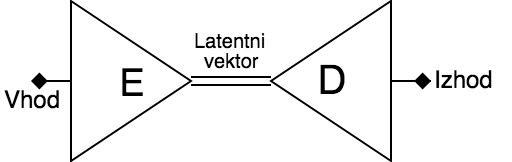
\includegraphics[width=0.35\textwidth]{images/autoencoder_schema.png}
 \caption[Idejna shema oblike autoenkoderja]{Idejna shema oblike autoenkoderja.}
  \label{fig:autoencoder-shape}
\end{figure}

V splošnem se bo v procesu kodiranja in odkodiranja vedno zgodila izguba informacij, saj je latentni prostor manjše dimenzije kot vhodni podatek. Naprimer, sliko velikost 28x28 točk stisnemo v vektor velikost 10x1. 
\\
Nevronsko mrežo učimo tako, da želimo da je rekonstuiran podatek čim bolj podoben vhodnemu. Na prvi pogled se zdi, da je uporabnost avtoenkoderjev omejena na kompresijo podatkov, vendar obstaja velika uporabnost na področju generativnih modelov. 
Ker je latentni prostor manjše dimenzije, prisilimo mrežo, da v latentni prostor zakodira čim več informacije in tako ohrani najpomembnejše značilke na slikah. \\
V praksi je to koristno v namene razšumljanja slik, inpaintinga. V teh primerih mrežo naučimo da iz nepopolnih (manjkajočih, šumnatih) slik zgenerira čiste slike. 
\\
V najbolj enostavni obliki je autoenkoder sestavljen iz treh slojev. Vhodni sloj je polno povezav z edinim skritim slojem, ki je nato polno povezan z izhodnim slojem. 
V praksi je najpogostejša izboljšava osnovne arhitekture  oblika z več polnopovezanimi skritimi sloji, ki se zmanjšujejo v velikosti na strani enkoderja in povečujejo na strani dekoderja. 
Če delamo s podatki kot so slike, lahko polnopovezane sloje zamenjamo s konvolucijskimi sloji različnih velikosti. 
\\
Dimenzije skritih slojev in latentnega vektorja so odvisne od dimenzij vhodnih podatkov ter od tipa podatkov s katerimi delamo. Parametri modela morajo biti prilagojeni našim podatkom in cilju, ki ga želimo doseči. 

\begin{figure}[ht]
  \centering
  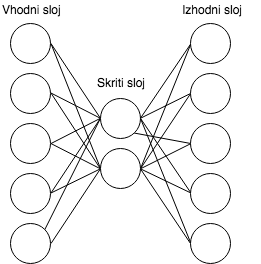
\includegraphics[width=0.35\textwidth]{images/autoencoder.png}
 \caption[Diagram najenostavnejšega autoenkoderja]{Diagram najenostavnejšega autoenkoderja.}
  \label{fig:autoencoder-diagram}
\end{figure}


\subsection{Generativne nasprotniške mreže}
Generativne nasprotniške mreže so bile prvič predstavljene v članku  \cite{gangoodfellow}, kjer je predstavljen algoritem tudi podkrepljen s teoretičnimi
dokazi. Glavna ideja algoritma je, da pomerimo generativni model proti nasprotniku, ki določa ali je generiran rezultat podoben tistemu, ki ga želimo modelirati. 
Predstavljamo si lahko bitko med ponarejevalcem denarja in strokovnjakom, ki določa ali je kos denarja pristen. Želimo, da oba akterja skozi iterativni nasprotniški proces izboljšujeta drug drugega. \\ I
dejno shemo  mreže lahko vidimo na sliki \ref{fig:gan-diagram}. To lahko primerjamo s shemo autoenkoderja  \ref{fig:autoencoder-shape} in razlike v arhitekturi so očitne. 
\begin{figure}[ht]
  \centering
  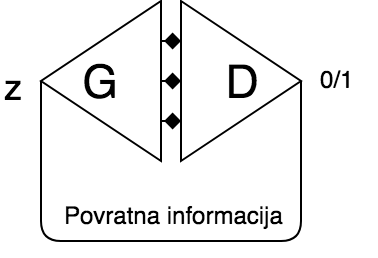
\includegraphics[width=0.35\textwidth]{images/gan_schema.png}
 \caption[Diagram strukture autoenkoderja ]{Generator na vhod dobi šum $z$ iz katerega zgenerira rezultat, diskriminator pa pove ali misli, da je slika iz učne množice ali ne}
  \label{fig:gan-diagram}
\end{figure}


Rečemo, da sta oba  diskriminator kot generator večslojni nevronski mreži. Matematično gledano, želimo naučiti generator G, da bo proizvajal vzorce, katerih porazdelitev je podobna porazdelitvi podatkov, katere želimo modelirati. Da bi se naučili porazdelitev generatorja $p_g$ na podatkih $x$, definiramo priorni porazdelitev $p(z)$, kjer $z$ predstavlja vektor šuma.\\ Preslikavo v prostor podatkov predstavimo z $G(z;\theta_g)$, kjer je G odvedljiva funkcija, ki jo predstavlja večslojna nevronska mreža in $\theta_g$ njeni parametri.  Prav tako definiramo $D(x,\theta_d)$, katerega izhod je skalar $D(x)$ ,ki predstavlja verjetnost, da je $x$ prišel iz podatkov in ne iz  $p_g$ (torej ni bil generiran s pomočjo generatorja). Hočemo torej, da diskriminator za vhod vedno pravilno določi ali je prišel iz množice realnih podatkov oz. ali je bil generiran s pomočjo generatorja $G$. To zapišemo kot: 
\begin{equation}
\label{eq:gan-main}
 \min_G\max_DV(D,G) = \mathbb{E}_{x \sim p_{data}(x)}[\log{D(x)}] + \mathbb{E}_{z \sim p_z(z)}[\log{(1-D(G(z)))]}
\end{equation}

Psevdokoda algoritma, ki uporablja gradientni spust za implementacijo našega generativnega nasprotniškega modela, je sledeča: 
\begin{algorithm}
\caption{Učenje generativnega nasprotniškega modela s pomočjo gradientnega spusta}\label{euclid}
\begin{algorithmic}[1]
\For{št. iteracij treninga}
\For{$k$ korakov}
	\State {Vzorči $m$ vzorcev  $ \{ z^{(1)},\dots ,z^{(m)} \} $ iz priorne porazdelitve $p_g(z)$}
	\State {Vzorči $m$ vzorcev  $ \{ x^{(1)},\dots,x^{(m)} \} $ iz porazdelitvne podatkov $p_{data}(x)$ } 
	\State {Posodobi diskriminator z vzpenjanjem po gradientu
				$$ \nabla \theta_d \frac{1}{m}\sum_{i=1}^{m}[\log{D(x^{(i)})} + \log{(1-D(G(z^{(i)}))}] $$}
\EndFor
	\State {Vzorči $m$ vzorev  $ \{ z^{(1)},\dots ,z^{(m)} \} $ iz priorne porazdelitve $p_g(z)$ }
	\State {Posodobi generator s pomočjo gradientnega spusta
				$$ \nabla \theta_d \frac{1}{m} \sum_{i=1}{m}\log{(1-D(G(z^{(i)})))}$$}
\EndFor
\end{algorithmic}
\end{algorithm}

Parameter $k$ za število iteracij notranje zanke, določimo glede na eksperimentalne korake. Pove nam kolikokrat naredimo korak optimizacije diskriminatorja za vsak korak generatorja. 
Želimo, da generator in diskriminator ostajata v ravnovesju. Če eden od njiju postane preveč učinkovit, težko pride do nadaljnjega izboljšanja v kvaliteti rezultatov, kar je tudi ena glavnih slabosti tega pristopa.  
Na začetku učenja, ko je G slab, se v praksi lahko zgodi, da $D$ z lahkoto zavrne vse generirane vzorce, saj so očitno različni od podatkov iz učne množice. V tem primeru se vrednost $\log(1-D(G(z)))$ močno poveča in težko najdemo globalni minimum. Da se izognemo temu problemo, reformuliramo problem tako, da namesto minimizacije  $\log(1-D(G(z)))$ učimo $G$, da maksimizira $\log{D(G(z))}$. To nam omogoča. da na začetku učenja dobimo močnešje gradiente, ki omogoča boljše premike v smer optimalne rešitve. 
\\
Ena od možnih razširitev omenjenih v članku je razširitev na pogojni generativni model $p(x | c)$, kar  dobimo tako, da dodamo pogoj $c$ na vhod tako generatorju kot diskriminatorju.  


\subsection{Variacijski autoenkoder}
Eden od glavnih pristopov pri generativnem strojnem učenju je uporaba variacijskih autoenkoderjev \cite{kingma2013auto}.  TI so posplošitev autoenkoderja, kjer  enkoder pogojimo da ustvarjeni latentni vektorji okvirno sledijo normalni porazdelitvi. Generiranje novih slik je torej samo vzorčenje iz  normalne porazdelitve,
z določeno srednjo vrednostjo in standardno deviacijo, ki jo dobimo iz mreže. Vedno je potreben kompromis med rekonstrukcijsko napako in prileganjem normalni porazdelitvi. 
Statistično gledano imamo spremenljivko $z$, katera generira $x$. Izračunali bi radi $p(z|x) = \frac{p(x|z)p(z)}{p(x)}$. Izkaše se, da je izračun te porazdelitve v praksi problematičen, zato aproksimiramo to porazdelitev z porazdelitvijo $q(z|x)$, ki ji je podobna in jo znamo izračunati. Za mero podobnosti med dvema porazdelitvama pa uporabimo KL divergenco. 
V naslednjem delu predstavimo bolj natančno in formalno izpeljavo variacijskega autoenkoderja. 
 \\
Predstavljajmo si množico $ X = \{x^{(i)}\}_{i=n}^N$, ki vsebuje $N$ neodvisnih in enakomerno porazdaljenih slučajnih spremenljivk $x$. Predpostavimo, da so podatki generirani s pomočjo nekega naključnega procesa, ki vključuje slučajno spremenljivko $z$, ki pa jo ne vidimo. \\
Ta proces je sestavljen iz dveh korakov 
\begin{enumerate}
\item Vrednost $z^{(i)}$ je generirana iz predhodne porazdelitve $p_{\theta^*}(z)$
\item Vrednost $x^{i}$ je generirana iz pogojne porazdelitve $p_{\theta^*}(x|z)$
\end{enumerate}

Predpostavimo, da $p_{\theta^*}(z)$ in $p_{\theta^*}(x|z)$ prihajata iz družine porazdelitev 
$p_{\theta}(z)$ in $p_{\theta}(x|z)$ in da je njihova gostota verjetnosti povsod odvedljiva glede na parametra $\theta$ in $z$.  
V praksi so vrednosti $z^{(i)}$ ter vrednost $\theta^*$ neznane. \\
Zanima nas rešitev, ki deluje tudi v primeru večje podatkovne množice ter kadar je intergral marginalne verjetnosti 
$p_\theta (x) = \int p_\theta (z)p_\theta (x|z)dz$ neobladljiv ( ne moremo ga odvajati oz. izračunati) in kjer je posteriorna gostota
$p_\theta(z|x) = p_\theta(z|x)p_\theta(z)/p_\theta(x)$ neobvladljiva. Ta dva primera, se velikokrat pojavljata prav v nevronskih mrežah z nelinearnimi skritimi sloji. 
\\
Pristop z variacijskimi autoenkoderji nam omogoča učinkovito ocenjevanje parametrov $\theta$, kar nam omogoča generiranje umetnih podatkov, ki so podobni naravnim. Kadar imamo neko vrednost $x$ ter izbrane parametre $\theta$, nam VAE omogoča 
dobiti aproksimacijo latentne spremenljivke $z$. To se uporablja v namene kodiranja, kjer informacije iz $x$ zakodiramo v $z$. 
Še ena od uporabnih lastnosti pa je aproksimiranje inference spremenljivke $x$, kar nam omogoča uporabo v smeri razšumenja, "inpaintinga" itd. 
\\
Uvedemo prepoznavni model $q_\phi(z|x)$, ki je aproksimacija $p_\theta(z|x)$. Izpeljali bomo metodo, ki se  $\phi$ nauči skupaj s parametri $\theta$
Neopazovano spremenljivko $z$, si lahko predstavljamo kot zakodirano informacijo.  Zato model $q_\phi(z|x)$ imenujemo \textbf{enkoder}, saj nam glede na podatek  $x$ izračuna porazdelitev možnosti $z$, ki bi lahko generirale ta podatek. 
Analogno bomo $p_\theta(x|z)$ imenovali \textbf{dekoder}, saj nam iz $z$ producira porazdelitev čez vrednosti $x$.  
\\
Izpeljemo lahko spodnjo mejo: 
\begin{equation}
 \mathcal{L}(\theta,\phi,x^{(i)}) = - D_{KL}(q_\phi(z|x^{(i)})||p_\theta(z)) + \mathbb{E}_{q\phi (z|x^{(i)})}[\log{p_\theta(x^{(i)}|z)}] 
\end{equation}

ki jo želimo optimizirati glede na parametre $\phi$ in $\theta$.  Zaradi velike variance gradienta, je naivna Monte Carlo metoda, za ta primer neučinkovita in potrebujemo boljšo metodo. 
\\
Zanima nas cenilka za  spodnjo mejo $\mathcal{L}$ in njene odvode. Upoštevajoč nekaj pogojev, ki so bolj natančno razloženi v \cite{kingma2013auto}, lahko reparametriziramo $\tilde{z} \sim q_\phi(z|x)$ z odvedljivo preslikavo šuma $\epsilon$, torej 
$\tilde{z} = g_\phi(\epsilon,x)$, kjer velja $\epsilon \sim p(\epsilon)$.
Sedaj lahko vpeljemo Monte Carlo aproksimacijo za pričakovano frednost neke funkcije $f(z)$, glede na $q_\phi(z|x)$. kot
\begin{equation}
 \mathbb{E}_{q_\phi(z|x^{(i)})}[f(z)] = \mathbb{E}_{p(\epsilon)}[f(g_\phi(\epsilon,x^{(i)}))] \simeq \frac{1}{L}\sum_{l=1}^{L}f(g_\phi(\epsilon^{(l)},x^{(i)})) 
\end{equation}

, kjer je $\epsilon^{(l)} \sim p(\epsilon)$. \\
To tehniko apliciramo na naš problem in dobimo cenilko $\tilde{\mathcal{L}}^A(\theta,\phi;x^{(i)}) \simeq \mathcal{L}(\theta,\phi;x^{(i)})$  za katero velja 
\begin{equation}
\tilde{\mathcal{L}}^A(\theta,\phi;x^{(i)}) = \frac{1}{L} \sum_{l=1}^L \log{p_\theta (x^({i}),z^{(i,l)})}-\log{q_\phi (z^{(i,l)}|x^{(i)})}
\end{equation}
 kjer
 
 \begin{equation}
 z^{(i,l)} = g_\theta(\epsilon^{(i,l)},x^{(i)}) \text{ in } \epsilon^{(l)} \sim p(\epsilon)
 \end{equation}


Velikokrat lahko $KL-divergenco$ integriramo analitično, tako da je ocena z vzorčenjem potrebna le za rekonstrukcijsko napako. $\mathbb{E}_{q\phi(z|x^{(i)})}[\log{p_\theta(x^{(i)}|z)}$. KL-divergenco si lahko predstavljamo kot regularizacijski člen $\phi$, kar nam 
da drugo različico cenilke $ \widetilde{\mathcal{L}}^B(\theta,\phi;x^{(i)}) \simeq \mathcal{L}(\theta,\phi;x^{(i)}) $ ki je definirana kot 
\begin{equation}
  \widetilde{\mathcal{L}}^B(\theta,\phi;x^{(i)}) = - D_{KL}(q_\phi(z|x^{(i)})||p_\theta(z)) + \frac{1}{L}\sum_{l=1}^L(\log{p_\theta(x^{(i)}|z^{(i,l)}))}  
\end{equation}

in velja 
\begin{equation}
 z^{(i,l)} = g_\phi(\epsilon^{(i,l)},x^{(i)}) \text{ in }  \epsilon^{(l)} \sim p(\epsilon)
\end{equation}
\\
Če Iz podatkovnem množice $X$ z $N$ elementi vzorčimo po $M$ vzorcev, lahko skonstruiramo cenilko osnovano na minisvežnjih: 
\begin{equation}
 \mathcal{L}(\theta,\phi;X) \simeq \widetilde{\mathcal{L}}(\theta,\phi;X^M) = \frac{N}{M}\sum_{i=1}^M \widetilde{\mathcal{L}}(\theta,\omega;x^{(i)}) 
\end{equation}

Minisveženj $X^M = \{ x^{(i)} \}_{i=1}^M$ je naključno izbran vzorec velikosti $M$ iz množice $X$.
V psevdokodi je  algoritem predstavljen kot 
\begin{algorithm}
\caption{Minibatch verzija AEVB algoritma. Lahko se uporablja cenilka $\widetilde{\mathcal{L}}^A$ ali $\widetilde{\mathcal{L}}^B$ }\label{minibatch-aevb}
\begin{algorithmic}[1]
\State $\theta,\phi \leftarrow$  inicializacija parametrov
\Repeat 
	\State $X^M \leftarrow$ Naključen minibatch $M$ vzorcev iz $X$
	\State $\epsilon \leftarrow$ Naključni vzorec šuma iz porazdelitve $p(\epsilon)$
	\State $g \leftarrow \nabla_{\theta,\phi}\widetilde{\mathcal{L}}^M(\theta,\phi;X^M,\epsilon)$ (Gradient minibatch cenilke)
	\State $\theta,\phi \leftarrow$ Posodobimo parametre s premikom v smeri gradienta (SGD ali ADAGRAD)	  
\Until parametra $(\theta,\phi)$ skonvergirata \\
\Return $\theta,\phi$
\end{algorithmic}
\end{algorithm}

\subsection{Nasprotniški autoenkoder}
Nasprotniški autoenkoderji \cite{adverserialautoencoders} so razširitev autoenkoderjev in so po svoje zasnovi precej podobni variacijskim avtoenkoderjem.  
Glavna razlika se pojavi v načinu zagotavljanja porazdelitve latentnega vektorja. Variacijski autoenkoder uporablja KL-divergenco kot vodilo za vodenje pravilne porazdelitve, medtem ko se
pri nasprotniških avtoenkoderjih uporablja nasprotniško učenje, kjer želimo s pomočjo diskriminatorja doseči isti cilj. 
\\
Naj bo $x$ vhodni podatek, $z$ latentni vektor autoenkoderja in $p(z)$ porazdelitev kateri želimo da koda $z$ sledi. Definirajmo $q(z|x)$ kot porazdelitev enkoderja, $p(x|z)$ kot porazdelitev dekoderja, $p_d(x)$ kot porazdelitev podatkov ter 
$p(x)$ kot porazdelitev našega modela. Enkoder definira porazdelitev $q(z)$ na latentnem vektorju kot  
\begin{equation}
 q(z) = \int_x q(z|x)p_d(x)dx 
\end{equation}
Nasprotniški autoenkoder je autoenkoder, ki je regulariziran z ujemanjem med $q(z)$ in $p(z)$. \\
Nasprotniška mreža je zadolžena za vodenje porazdelitve $q(z)$ proti $p(z)$, medtem ko je autoenkoder zaslužen za minimiziranje rekonstrukcijske napake. 
Velja, da je generator nasprotniške mreže tudi enkoder autoenkoderja $q(z|x)$, ki je zadolžen da prelisiči diskriminator, da ne loči med $q(z)$ in $p(z)$.
Učenje vedno izvajamo v dveh delih, najprej učimo nasprotniško mrežo (diskriminator) in s tem regulariziramo porazdelitev latentnega vektorja. S tem se posodobi tudi generator mreže, ki je hkrati enkoder autoenkoderja tako, da bolje zmede diskriminator.  V 
drugem koraku pa učimo autoenkoder in s tem izboljšujemo rekonstrukcijsko napako. 
\\
Možnih je nekaj različnih izbir za enkoder $q(z|x)$
\begin{itemize}
\item \textbf{Deterministični} Predpostavimo, da je $q(z|x)$ deterministična funkcija $x$-a. V tem primeru je enkoder podoben enkoderju standardnega autoenkoderja in edini vir stohastičnosti (nepredvidljivosti)  v $q(z)$ ostane učna množica $p_d(x)$.
\item \textbf{Normalno porazdeljeni} Privzamemo, da je $q(z|x)$ normalna porazdelitev, katere srednja vrednost in varianca je dobljena iz enkoderja. Velja torej:
\begin{equation}
z_i \sim \mathcal{N}(\mu_i(x),\sigma_i(x))
\label{eq:aae-normal}
\end{equation}


V tem primeru stohastičnost dobimo tako iz učne množice kot iz naključnosti naravne porazdelitve.
\item \textbf{Univerzalni aproksimator} To si predstavljamo kot posplošitev prejšne možnosti. Cilj je, da  $q(z|x)$ naučimo kot univerzalni aproksimator. Naj bo enkoder funkcija $f(x,\eta)$, ki na vhod dobi $x$ in  naključni šum $\eta$ s fiksno porazdelitvijo, potem lahko vzorčimo iz katerekoli posteriorne porazdelitve $q(z|x)$, tako da evaluiramo $f(x,\eta)$ pri različnih vzorcih 
$\eta$. Matematično gledano, predpostavimo da velja $q(z|x,\eta)$ = $\delta(z-f(x,\eta))$ in 
\begin{equation}
q(z|x) = \int_{\eta} q(z|x,\eta)p_\eta(\eta)d \eta \implies q(z) = \int_x \int_{\eta} q(z|x,\eta)p_{d}(x)p_{\eta}(\eta)d \eta dx 
\end{equation}

Tu je stohastičnost  v $q(z)$ dobljena tako iz učne množice kot iz šuma $\eta$ na vhodu enkoderja. V tem primeru nismo več omejeni na naravno porazdelitev, ampak si lahko izberemo kakršnokoli porazdelitev želimo, saj to določuje porazdelitev šuma $\eta$. 
\end{itemize}

Nasprotniški autoenkoder je mogoče razširiti v pogojno obliko kjer vsem učnim vzorcem dodelimo oznako kateremu razredu pripadajo. 
Na vhod diskriminatorja dodamo one-hot (?) oznako, ki predstavlja razred, kateremu vzorec pripada. 
Ko enkoder izračuna latentni vektor združimo oznako skupaj s latentnim vektorjem in to podamo dekodirnemu delu mreže. 

\section{Staranje obrazov}
Področje staranja obrazov je pred razmahom globokega učenja večinoma uporabljalo modelne pristope \cite{fu2010age}. S pomočjo modeliranja strukture človeškega obraza in povezane anatomije se je želelo simulirati vplive staranja na človeški videz. 
Kot predpogoj potrebujemo način za modeliranje človeškega obraza in njegovih mimik. Veliko raziskovalnega dela v tej smeri pride iz področja animacije.  Ločimo tri glavne vrste modelov in sicer \textbf{geometrične, image-based,appearance-based}. 
\\Pri geometričnih modelih ustvarimo mrežo ključnih točk na človeškem obrazu. S transformacijami nad temi točkami pa lahko simuliramo mimiko in staranje. Potrebujemo način, ki nam ob transformacij še vedno ohrani osnovno strukturo objekta. 
Za to obstaja  več pristopov, eden od najbolj znanih pa je predstavljen v  \cite{cootes1995active}, in se tudi uporablja na podrčju zaznave ključnih točk na obrazu. 
\\
Slikovno osnovani modeli se trudijo ustvariti fotorealistične slike na podlagi drugih slik. Eden od primerov je prenos teksture iz ene slike na drugo s pomočjo precesiranja slikovnih signalov in geometričnega modeliranja \cite{liu2004image}. 
Podobne tehnike osnovane na prenašanju lastnostni iz prototipnega obraza se uporabljajo za prenos osvetlitve, izraza in starosti \cite{fu2006m}.
\\
Izgledni modeli  za razliko od prejšnjih dveh uporabljajo statistično učenje za izgradnjo modela. V večini primerov se iz velike baze podatkov zgradi generični prototipni model.   Uporablja se tAAM model \cite{cootes2001active}, ki ga s pomočjo učne množice naučimo
statistični model obraza. 
 \textbf{TUKAJ NADALJUJ --- PLACEHOLDER, KER NEVEM KAKO BI TO ZASTAVU} 
 \\
 
 Za razliko od zgoraj opisanih pristopov pa modernejši pristopi uporabljajo nevronske mreže za dosego istih ciljev.  Z uporabo generativnih model želimo učenje statističnega modela stranja prepustiti nevronski mreži, ki se na osnovi večje baze fotografij oseb različnih starosti 
 sama nauči kako poteka staranje človeškega obraza. 
\subsection{Staranje z uporabo pogojnih generativnih nasprotniških mrež}
 
Eden od pristopov, opisan v \cite{antipov2017face}, simulira staranje s pomočjo \textbf{pogojne  generativne  nasprotniške mreže}. 
Glavna ideja razdeli postopek na tri dele
\begin{enumerate}
\item Naučimo pogojno generativno nasprotniško mrežo
\item Glede na podano sliko $x$ starosti $y_0$, poišči latentni vektor $z^*$ pri katerem generator zgenerira sliko, ki je najbolj podobna podani. Torej želimo minimizirati razliko med $x$ in $\hat{x} = G(z^*,y_0)$
\item Staranje dosežemo tako, da generatorju ob optimalnem vektorju $z^*$ namesto originalne starosti podamo ciljno starost $y_{cilj}$, torej $x_{cilj} = G(z^*,y_{cilj})$. 
\end{enumerate}
Zelo pomembna je informacija o arhitekturi nevronske mreže, ki nam generira slike. Tukaj se znotraj mreže uporabljajo konvolucijski sloji v generatorju in dekonvolucije v diskimnatorju. Za doseganje stabilnosti učenja je priporočeno upoštevanje nekaterih osnovih smernic \cite{radford2015unsupervised}
\begin{itemize}
\item Vse pooling layerji (?) zamenjamo s koračnimi konvolucijami v diskriminatorju in obratno koračnimi (fractional strided) konvolucijami v generatorju
\item Paketna normalizacijo uporabljamo tako v generatorju kot v diskriminatorju
\item Pri bolj globokih arhitekturah ne smemo uporabljati polno povezanih slojev
\item V generatorju uporabljamo ReLU aktivacijski funkcijo v vseh slojih, razen v zadnjem
\item V diskriminatroju za vse sloje uporabljamo LeakyReLU aktivacijsko funkcijo
\end{itemize} 

V tem primeru generator na vhod sprejme vektor šuma $z$ dimenzije 100x1. Nato ga s pomočjo polnopovezanega  sloja in preoblikovanja  razširi na dimenzijo 1024x4x4, katero nato s pomočjo zaporedja obratno koračnih kovolucij spremenimo v dimenzijo slike, ki je 64x64x3. 
To je najbolje vidno na sliki \ref{fig:agecgan-generator}, ki nazorno prikaže arhitekturo. 
\\ 
Oblika diskriminatorja je simetrična tej, z razliko da  namesto obratno koračnih, uporabljamo koračne kovolucije z velikostjo  koraka 2. Ločite se tudi v tem, da je zadnji sloj v diskriminatorju  polnopovezan z velikostjo 1,
saj je cilj samo vračanje enega bita informacije.
\\
V drugem koraku želimo gelde na podano sliki $x$ starosti $y_o$ poiskati latentni vektor, ki ustvari sliko $\hat(x)$, ki je najboljši približek podani sliki $x$.  
V nasprotju z autoenkoderji, nam generativne nasprotniške mreže ne podajo možnosti za preslikavo slike $x$ z atributi $y$ v latentni vektor $z$. 
Imamo torej definirano preslikavo $f: (z,y) \mapsto x$ želimo pa dobiti preslikavo $f^{-1}: (x,y) \mapsto z$
\\
To lahko rešimo tako da naučimo enkoder $E$, nevronska mrežo zadolženo za  aproksimiranje $f^{-1}$.  
Najprej ustvarimo sintetično množico sto tisoč parov $(x_i,G(z_i,y_i))$, kjer so $z_i \sim N(0,I)$ naključni latentni vektorji ter $y_i \sim U$  enakomerno naključno izbrane oznake starostnih skupin. $G(z_i,y_i)$ je na učni množici obrazov in starostni 
naučena pogojna nasprotniška generativna mreža (CGAN). Enkoder je naučen tako, da minimiziramo evklidsko razdaljo med aproksimiranimi latentnimi vektorji $E(x_i)$ in $z_i$, kjer je $x_i = G(z_i,y_i)$
\\
Dobljeni rezultat je aproksimacija, ki jo želimo še dodatno izboljšati z uporabo optimizacijskih algoritmov. 
Cilj je minimizirati razdaljo med $x$ in $\hat(x)$.  Rezultati se precej razlikujejo odvisno od izbrane mere razdalje. 
Najenostavnejši pristop je uporaba evklidkse razdalje na razliki med slikovnimi točkami. 
Težava nastane, ker metoda gleda razlike med posameznimi piksli, ki velikokrat nimajo vpliva na ohranjanje identitete. Optimizacijska metoda npr. optimizira razlike v ozadju, frizuri ipd, čeprav bi želeli da se identiteti oseb čim bolj približati. 
Pomanjkljivost je tudi to, da nam slike zabriše. 
\\
Alternativni način je uporaba optimizacije ki ohranja identitete. Če imamo nevronsko mrežo $FR$  naučeno v namene razpoznave obrazov, lahko definiramo razdaljo kot razliko med reprezentacijah v tej mreži. 
V največ primerih gledamo evklidsko razdaljo med tenzorji definiranimi znotraj enega od slojev. 
Velja torej: 
\begin{equation}
z^* =  \argminB_z = || FR(x) -  FR ( \hat{x})  ||_{L_2}
\end{equation}


\begin{figure}[ht]
  \centering
  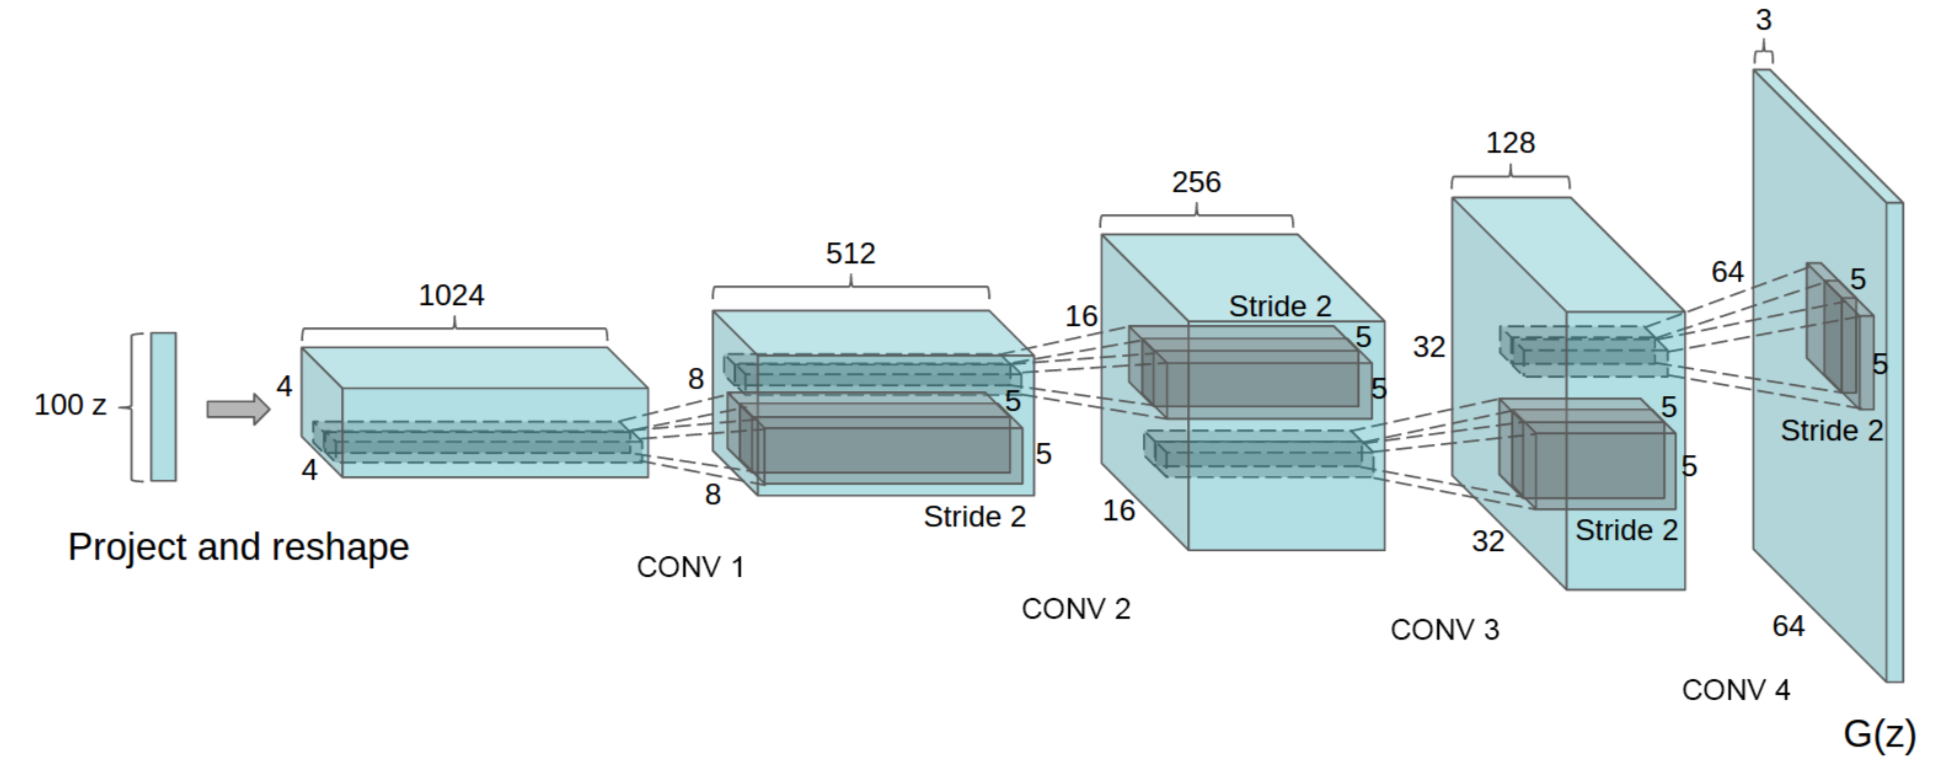
\includegraphics[width=0.7\textwidth]{cgan_architecture}
 \caption[Struktura generatorja uporabljenega v \cite{antipov2017face}]{Struktura generatorja uporabljenega v \cite{antipov2017face}.\\Vir: \cite{radford2015unsupervised}}
  \label{fig:agecgan-generator}
\end{figure}

Ker sta tako generator $G(z,y)$ kot nevronska mreža $FR$ odvedljiva glede na vhodne podatke, potem se optimizacijo lahko rešuje z uporabo \textbf{L-BFGS-B} algoritma, ki mu kot začetni približek podamo vrednost $z_0$, ki smo jo dobili iz enkoderja $E$. 
\subsection{Staranje z uporabo ponavljajočih nevronskih mrež}
Klasične ponavljajoče nevronske mreže podajajo dobre rezultate, kadar se ukvarjamo z zaporednimi podatki, kjer so členi medsebojno odvisni, to pa lahko izkoristimo za simuliranje postopka staranja \cite{wang2016recurrent}
Staranje si lahko predstavljamo kot zaporedje stanj, kjer je vsako novo stanje odvisno od prejšnjega. Starosti razdelimo na starostne skupine, cilj pa je najti prehode iz enega stanja v naslednjega. 
Postopek je sestavljen iz dveh glavnih korakov, kjer je prvi normalizacija obraznik slik, drugi pa staranje s pomočjo mreže. 
Pomembno je, da nam normalizacija ohrani podatke o starosti ter lepe prehode med starostnimi skupinami. 
Za dosego tega cilja se poslužimo tehnike, kjer normaliziramo slike sosednih starostnih skupin skupaj. Uporablja se  optični tok, saj  ohrani teksturne podrobnosti na slikah.  Podrobnosti in matematična formulacija  so podrobneje predstavljene  v 
\cite{wang2016recurrent}. 
Ko imamo slike normalizirane, se poslužimo ponavljajoče nevronske mreže, za izvajanje postopka staranja. 
Osnovna komponenta mreže so dvoslojna GRU (gated recurrent unit) vrata, kjer spodnji GRU zakodira vhodni obraz v skrito visokodimenzionalno reprezentacijo, ki jo zgornji del odkodira v postaran obraz. Kot našo kriterijsko funkcijo 
določimo razliko med vhodno sliko in referenčno sliko. Uteži postopoma povečujemo tako, da ima največjo težo razlika med najstarejšo starostno skupino in referenco. S tem omogočimo bolj realne prehode med stanji.



\subsection{Staranje s pogojnim nasprotniškim autoenkoderjem}
Predpostavimo da slike oseb pri različnih starostih ležijo na mnogoterosti $\mathcal{M}$. Premikanje po tem prostoru v določeni smeri nam ohrani identiteto, kljub temu da se starost spreminja. Želimo določiti 
 preslikavo med nižjedimenzionalnim latentnim prostorom in mnogoterostjo, saj je direktna preslikava med sliko in mnogoterstjo pretežka za modeliranje. 
 \\ 
 Imamo sliko obraza $x$, ki jo enkoder $E$ preslika v latentno reprezentacijo $z$, ki jo nato združimo z informacijo o starosti osebe $l$. S tem dobimo točko na $\mathcal{M}$. Glavna ideja je, da sta v latentnem prostoru informaciji o identiteti $z$ in starosti $l$ ločeni. To pomeni, da lahko samo spremenimo starost in s tem ohranimo identiteto osebe. S pomočjo generatorja $G$ to preslikamo nazaj v prostor slik, ki so človeku berljive. 
Za enkoder uporabimo konvolucijsko nevronsko mrežo, kjer se za namene downsamplinga (?) uporablja koračenje s korakom 2, kot je priporočeno v \cite{radford2015unsupervised}. Podobno velja za generator. 
Imamo tudi dva diskriminatorja: 
\begin{itemize}
\item $D_z$ je povezan z enkoderjem in skrbi, da latentni vektorji $z$ sledijo normalni porazdelitvi. S tem želimo prisiliti $E$ da je latentni prostor enakomerno zapolnjen.
\item $D_{img}$ prisili generator, da so rezultati fotorealistični, še posebej  se to vidi pri teksturi starejših obrazov.  
\end{itemize}

Pri podanem latentnem vektorju $z$ ter oznaki $l$, nam generator $G$ ustvari novo sliko $\hat{x} = G(z,l) = G(E(x),l)$. Želimo, da $\hat{x}$ leži na na $\mathbb{M}$ in ima isto identiteto kot $x$. 
Matematično je naš  cilj  dobiti rešitev enačbe 
\begin{equation}
 \min_{E,G} \mathcal{L}(x,G(E(x),l))
\end{equation}
 ter hkrati posrbeti, da je $z$ normalno porazdeljen ter da je kriterij diskriminatorja $D_{img}$ čim bolj izpolnjen.\\
 Porazdelitev učnih podatkov definiramo kot $p_{data}(x)$ in porazdelitev $z$ definiramo kot $q(z|x)$. Naj bo $p(z)$ priorna porazdelitev, potem z $z^* \sim p(z)$ definiramo vzorčenje iz $p(z)$. 
 Skupno učenje $E$ in $D_z$ predstavimo s kriterijsko funkcijo 
 \begin{equation}
  \min_E \max_{D_z}\mathbb{E}_{z^* \sim p(z)}[\log{D_z(z^*)}] + \mathbb{E}_{x \sim p_{data}(x)}[log(1-D_z(E(x)))]
 \end{equation}
 Analogno lahko definiramo kriterijsko funkcijo za učenje diskrimanatorja $D_{img}$ in generatorja $G$ z oznako $l$ kot  
 
\begin{equation}
 \min_G \max_{D_{img}} \mathbb{E}_{x,l \sim p_{data}(x,l)}[\log{D_{img}(x,l)}] + \mathbb{E}_{x,l \sim p_{data}(x,l)}[\log(1-D_{img}(G(E(x),l)))] 
\end{equation} 

Vse skupaj sedaj seštejmo in združimo v celotno kriterijsko funkcijo sistema

\begin{equation}
\begin{aligned}
 \min_{E,G} \max{D_z,D_{img}} \lambda \mathcal{L}(x,G(E(x),l))   \\
+ \mathbb{E}_{z^* \sim p(z)}[\log{D_z(z^*)}]  \\
+ \mathbb{E}_{x \sim p_{data}(x)}[log(1-D_z(E(x)))]   \\
+ \mathbb{E}_{x,l \sim p_{data}(x,l)}[\log{D_{img}(x,l)}]  \\ 
+ \mathbb{E}_{x,l \sim p_{data}(x,l)}[\log(1-D_{img}(G(E(x),l)))]
\end{aligned}
\end{equation}



\chapter{Implementacija}
Med raziskovanjem načina za doseganje najboljših rezultatov staranja in pomlajevanja smo se poslužili različnih pristopov, ki jih bomo predstavili v tem poglavju. Predstavili bomo teoretično podlago vsakega od njih ter dosežene rezultate. Analizirali bomo pomanjkljivosti in težave pri implementaciji.  
\\
Za implementacijo različnih modelov, je bila uporabljena programska knjižnica \textbf{Keras 2.0.0}, ki v ozadju uporablja \textbf{Tensorflow 1.0.0}. Za doseganje enakovrednih rezultatov je verzija pomembna, saj lahko starejše ali novejše različice dajejo bistveno drugačne rezultate. 

V vseh poizkusih, razen tam kjer je specifično navedeno drugače, smo za učno množico uporabljali bazo slik  UTKFace \cite{utkface}, ki vsebuje 20000 slik oseb različnih etničnih izvorov, spola ter starosti. 
Slike v bazi so obrezane ter poravnane ter vsebujejo slike oseb pri različnih osvetlitvah, obraznih mimikah ter stopnjah pokritosti.
Pomembna lastnost je porazdelitev starosti v bazi, ki jo uporabljamo za učenje. V tabeli \ref{tbl: utkface-distribution} vidimo, da je baza neuravnovešena proti starostnim skupinam med 20 in 40 let. Prav tako je manjše število slik ljudi starejših od 70 let, kar pa je za naše potrebe sprejemljivo, saj nam staranje do ekstremnih starosti ni poglavitnega pomena. 
\\
Pri implementaciji se je pojavil očiten problem pomanjkanja primerne podatkovne baze za učenje naših modelov. Potrebovali bi podatkovno bazo, ki spremlja osebo skozi proces staranja, torej kjer imamo fotografije iste osebe pri različnih starostih. Poleg tega pa bi želeli, da te fotografije osebo dokumentirajo od najmlajših do poznih let. Edina  prosto dostopna podatkovna baza, ki se približa tem kriterijem je \textbf{FG-NET database}, 
% Please add the following required packages to your document preamble:
% If you use beamer only pass "xcolor=table" option, i.e. \documentclass[xcolor=table]{beamer}
\begin{table}[ht]
\centering
\begin{tabular}{|c|c|}
\hline
\multicolumn{1}{|l|}{{\color[HTML]{333333} \textbf{Starostna skupina}}} & \multicolumn{1}{l|}{{\color[HTML]{333333} \textbf{Število slik v bazi}}} \\ \hline
{\color[HTML]{333333} 0-10}                                             & {\color[HTML]{333333} 3062}                                              \\
{\color[HTML]{333333} 10-19}                                            & {\color[HTML]{333333} 1531}                                              \\
{\color[HTML]{333333} 20-29}                                            & {\color[HTML]{333333} 7344}                                              \\
{\color[HTML]{333333} 30-39}                                            & {\color[HTML]{333333} 4537}                                              \\
{\color[HTML]{333333} 40-49}                                            & {\color[HTML]{333333} 2245}                                              \\
{\color[HTML]{333333} 50-59}                                            & {\color[HTML]{333333} 2299}                                              \\
{\color[HTML]{333333} 60-69}                                            & {\color[HTML]{333333} 1318}                                              \\
{\color[HTML]{333333} 70-79}                                            & {\color[HTML]{333333} 699}                                               \\
{\color[HTML]{333333} 80-89}                                            & {\color[HTML]{333333} 504}                                               \\
{\color[HTML]{333333} \textgreater 90}                                  & {\color[HTML]{333333} 169}                                               \\ \hline
\end{tabular}
\caption{Porazdelitev starosti v bazi UTKFace }
\label{tbl: utkface-distribution}
\end{table}

ki pa ima žal kar nekaj očitnih pomanjkljivosti. 
Največja od njih je majhna velikost podatkovne baze, saj obsega fotografije le približnost 80 različnih oseb, ter 1000 fotografij skupno. Prav tako je težava v tem, da je večino fotografij osebe pri različnih starostih posneto v časovnem intervalu nekaj let, kar nam ne omogoča določanja učinka dolgoročnega staranja. \\
Ena od podatkovnih baz, ki naj bi zadostila pogojem je \textbf{Morph} \cite{ricanek2006morph}, ki pa je plačljiva in ni prosto dostopna, zatorej je nismo mogli uporabiti. 

\section{Pogojna generativna nasprotniška mreža}
\subsection{Teoretično ozadje}
Kot je že bilo omenjeno v \cite{gangoodfellow} je ena od najbolj osnovnih razširitev GAN modelov, razširitev na pogojno mrežo, ki je bila natančneje formalizirana v \cite{mirza2014conditional}.
Ideja je enostavna, mrežo lahko razširimo v pogojni model tako, da pogojimo tako diskriminator kot generator z oznako informacije $y$. To informacijo podamo kot dodaten vhodni sloj obema deloma mreža. V praksi za $y$ največkrat uporabljam zapis v obliki angl. one-hot vektorja, ki nam pove kateremu razredu pripada določena informacija. 
\\
Formalno se enačba \ref{eq:gan-main}, ki opisuje nasprotniško delovanje dveh delov mreže osnovne oblike, sedaj razširi v

\begin{equation}
\min_G \max_D V(D,G) = \mathbb{E}_{x \sim p_{data}(x)}[\log{D(x|y)}] + \mathbb{E}_{z \sim p_z(z)}[\log{1-D(G(z|y)))}]
\end{equation}
\\
V primeru, da je arhitektura naše mreže sestavljena iz polnopovezanih slojev, lahko informacijo o razredu (oznaki) priključimo enemu od polnopovezanih slojev tako da jo enostavno dodamo na konec enega od slojev. V praksi to ponavadi naredimo v enem od prvih slojev mreže. 
\\
Kadar pa je naša mreža sestavljena samo iz konvolucijskih slojev, potem se moramo zateči h drugim načinom pogojitve  modela.  Konvolucijskemu sloju zaradi razlik v dimenzionalnosti namreč ni mogoče pripeti dodatne informacije o  razredu. V tem primeru uporabimo trik, kjer glede na razred, vsak vhod pomnožimo z določeno skalarno vrednostjo. To nam omogoči, da vhodne podatke glede na razred razpršimo po prostoru in tako dosežemo, da mreža razlikuje med različnimi razredi vhodnih podatkov.

\subsection{Implementacija}

V našem primeru smo želeli preizkusiti pogojno generativno  nasprotniško mrežo kot osnovni generativni model, nad katerim bi potem preizkušali nove metode. Začeli smo s polnopovezano arhitekturo, ki je najenostavnejša za implementacijo.  Na sliki \ref{fig:cgan-implementation-architecture} 

\begin{figure}[ht]
\centering
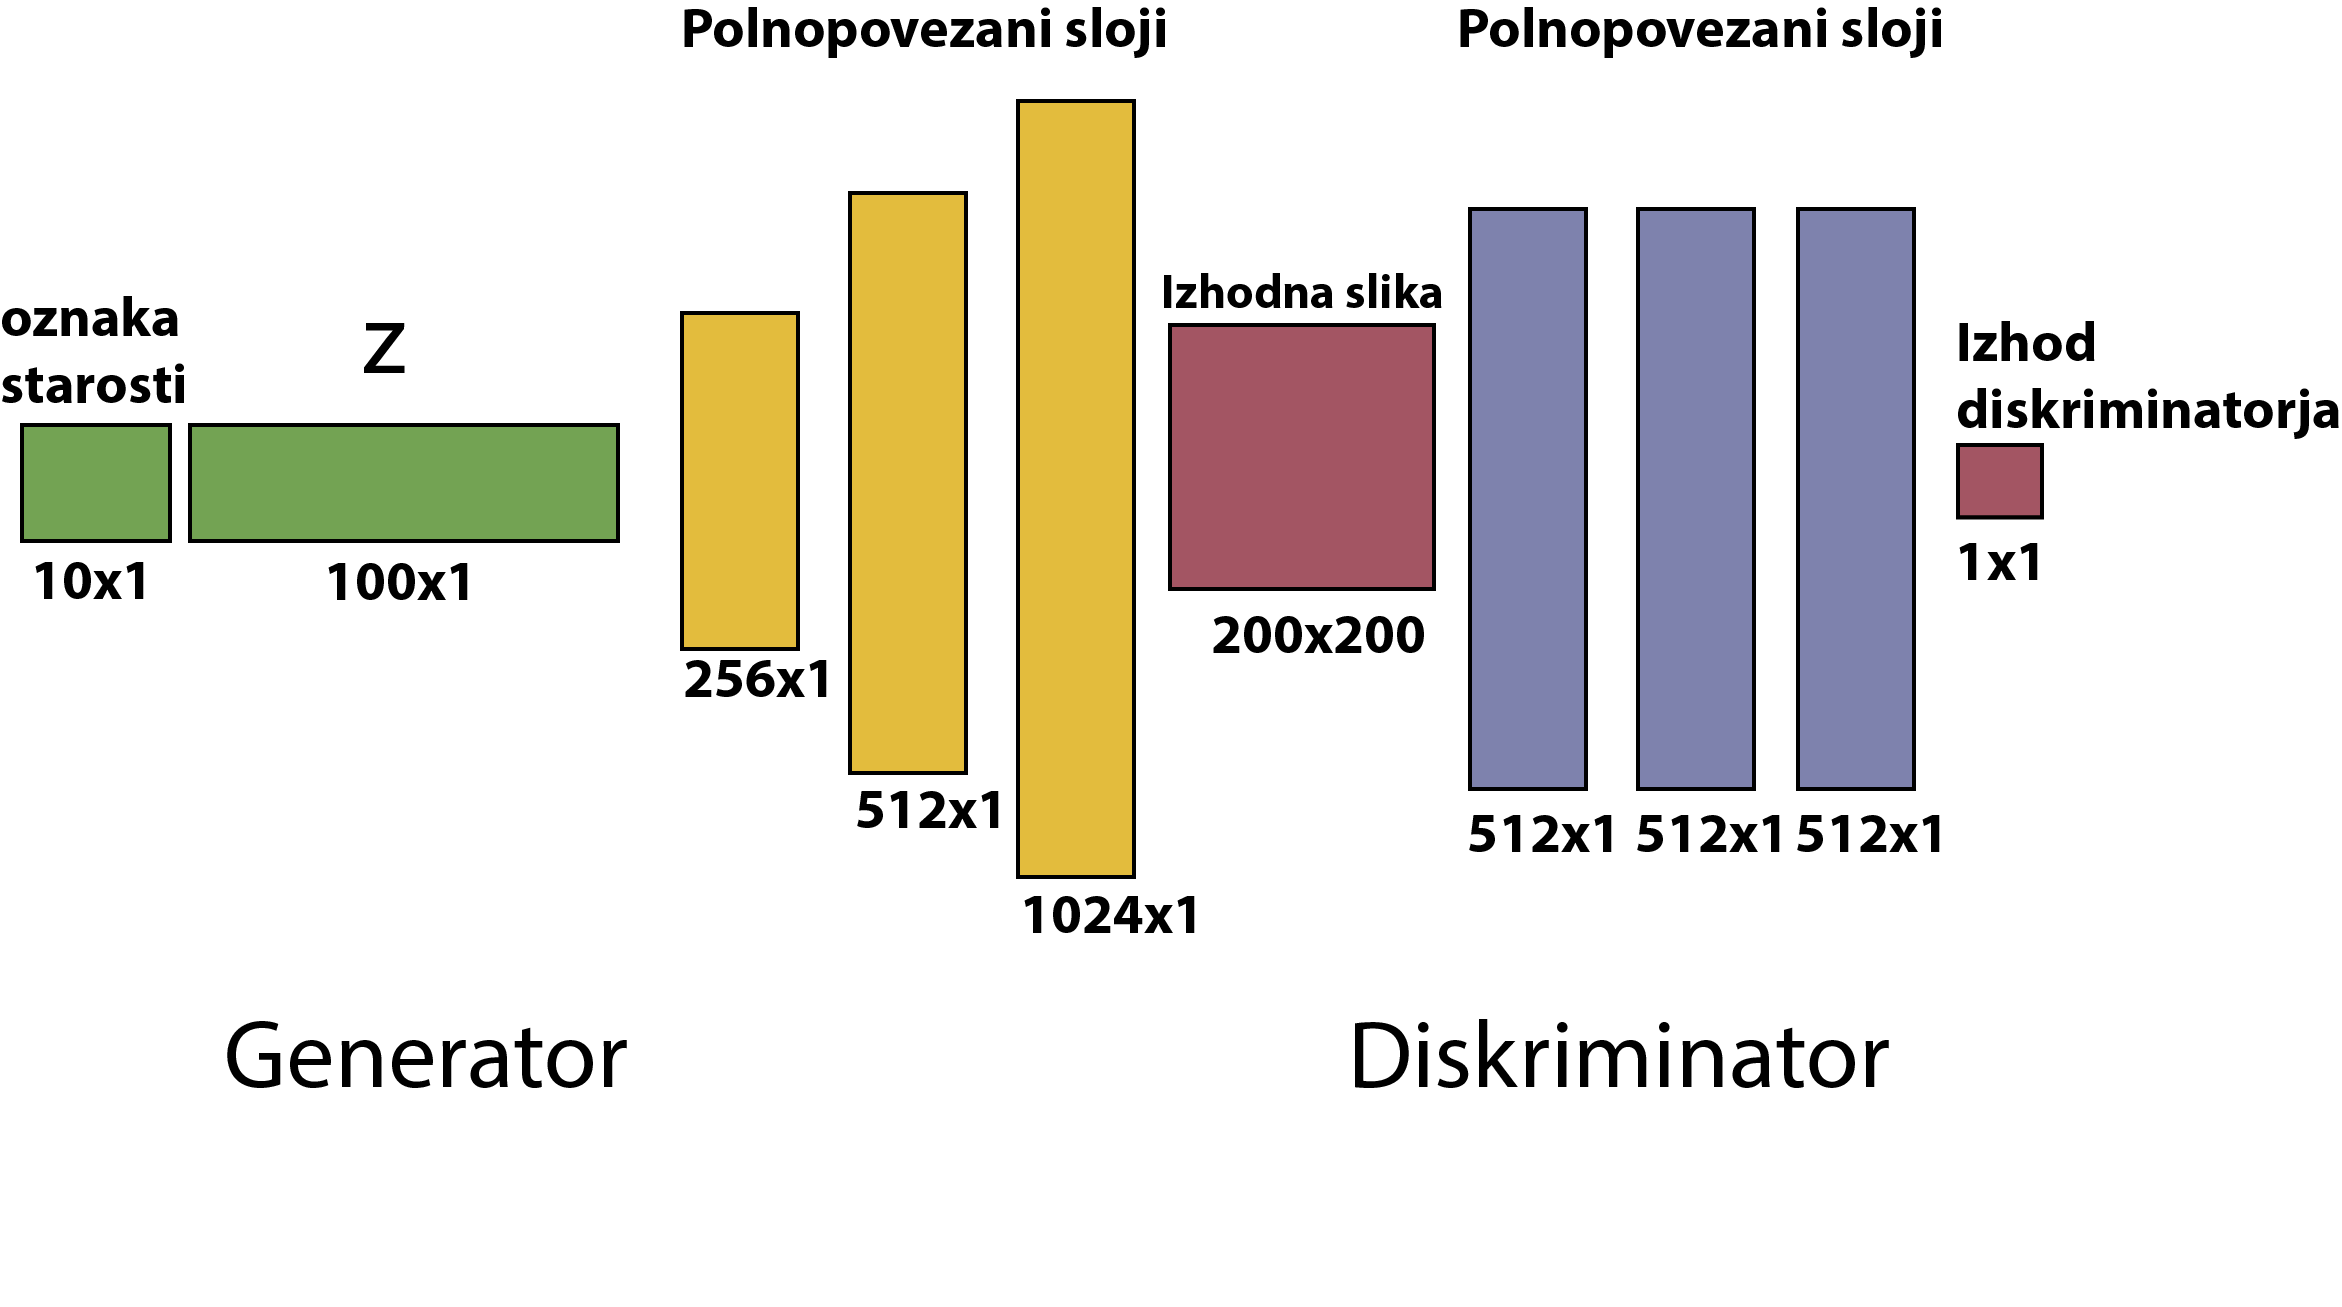
\includegraphics[width=0.95\textwidth]{images/cgan_dense_architecture.png}
\caption[Arhitektura polnopovezanega CGAN modela]{Arhitektura polnopovezanega CGAN modela}
\label{fig:cgan-implementation-architecture}
\end{figure}
vidimo arhitekturo našega modela. V generatorju je med polnopovezanimi sloji dodana še normalizacija svežnjev. Velja, da v vseh polnopovezaih slojih generatorja uporabimo \textbf{LeakyReLU} aktivacijsko funkcijo, razen v zadnjem, kjer se uporablja \textbf{tanh}. Pri diskriminatorju je med vsemi polnopovezanimi sloji dodan Dropout. Podobno kot prej, za aktivacijo uporabljamo \textbf{LeakyReLU} povsod, razen v zadnjem sloju, kjer se uporablja \textbf{sigmoid}.
\\
Arhitektura je neodvisna od velikosti vhoda, vendar smo se odločili, da bomo naš model preizkušali na slikah velikost 200x200 slikovnih točk.  
Kot kriterijsko funkcijo tako generatorja kot diskriminatorja uporabljamo binarno krosentropijo. Prav tako je to uporabljeno za skupni model. 
\\
Učenje je potekalo tako, da smo v vsaki iteraciji najprej učili diskriminator. Na vhod smo mu podali slike, ki so bile ustvarjene iz strani generatorja, skupaj z oznako starosti. Za te učne podatke smo želeli, da diskriminator na izhodu vrne vrednost 1. Kazali pa smo mu tudi naključno ustvarjene slike šuma, skupaj z oznakami starosti. V tem primeru, smo podali vrednost 0 kot zaželjeni izhod. 
Sledi učenje skupnega modela, kjer na vhod podamo vektor $z$ ter oznako o starosti na izhodu pa kažemo vektor enic. Kot optimizator smo  uporabljali  algoritem \textbf{ADAM} z nastavljeno hitrostjo učenja 0.005.Velikost svežnja smo nastavili na 32.

% -- MOVE TO RESULTS
Našo mrežo smo učili skozi 5 prehodov čez učno množico, vendar kot je vidno iz grafa učenja \ref{fig:cgan-loss} , je mreža imela težave s konvergenco in predvsem v drugi polovici učenja do vidnih izboljšav ni prišlo. 

\begin{figure}[ht]
  \centering
  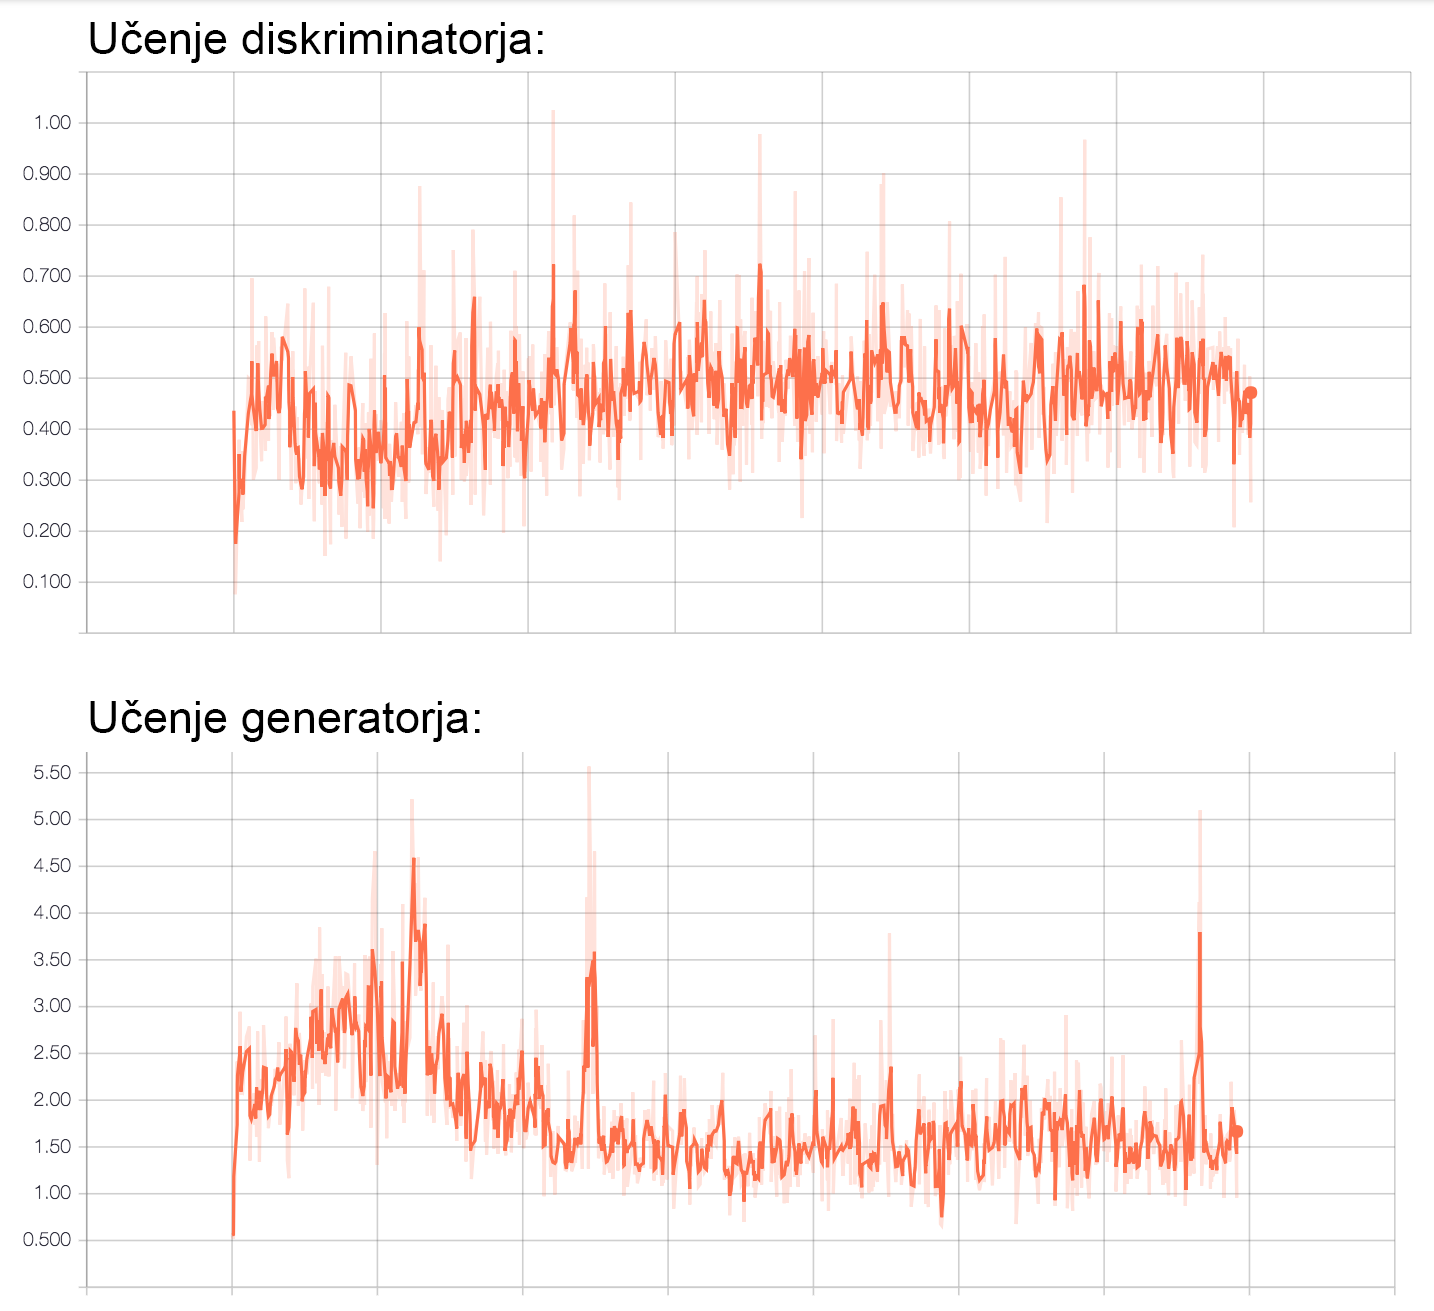
\includegraphics[width=0.75\textwidth]{images/cgan_loss.png}
 \caption[Graf učenja CGAN mreže s polnopovezano arhitekturo ]{Graf učenja CGAN mreže s polnopovezamo arhitekturo }
  \label{fig:cgan-loss}
\end{figure}


V nadalnjem delu se je izkazalo, da se težave s konvergenco pojavljajo pri večini generativnih modelov. Prav tako je težko doseči stabilnost, saj majhna sprememba hiperparametrov velikokrat močno vpliva na rezultate učenja. 
Če pogledamo generirane slike naključnih obrazov določenih starosti \ref{fig:cgan-generated}, vidimo da so dobljene slike zelo šumne.
\\ 
 Opazimo, da je mreži uspelo ujeti informacije o starostnih skupinah, vendar je vidno tudi, da so generirane slike določenih starostnih skupin precej slabše kvalitete kot ostale. Razlog je predvsem v tem, da je slik starejših oseb v bazi precej manj kot ostalih, kar privede do neravnovesja v kvaliteti slik različnih razredov. 
 \\
 Da bi izboljšali vizualno kvaliteto rezultatov, smo poskušali spremeniti arhitekturo obeh mrež v konvolucijsko obliko, ki je predlagana v \cite{radford2015unsupervised}. 
 Tudi tukaj pa se je pokazala nestabilnost osnovnega GAN pristopa. Na naši učni množici, je namreč mreža generirala slike, ki so vsebovale samo šum. Kljub empiričnem spreminjanju hiperparametrov in upoštevanja smernic iz literature, nam ni uspelo uspostaviti delovanja te mreže. 

 
\begin{figure}[ht]
  \centering
  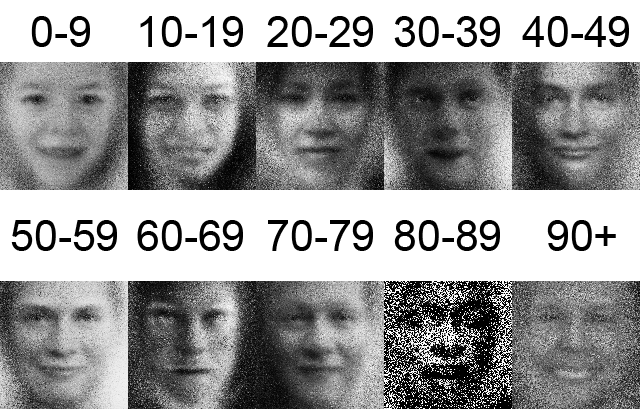
\includegraphics[width=0.6\textwidth]{images/cgan_generated.png}
 \caption[Ustvarjene obrazne slike s pomočjo CGAN mreže s polnopovezano arhitekturo ]{Ustvarjene obrazne slike s pomočjo CGAN mreže s polnopovezano arhitekturo }
  \label{fig:cgan-generated}
\end{figure}

\section{Pogojni Wasserstein GAN}
Eden od prvih preizkušenih modelov je bila pogojna različica wasserstein GAN \cite{arjovsky2017wasserstein} modela. Eden od glavnih izzivov pri učenju GAN modelov je nastabilnost učenja, kar pa naj bi wassersteinova različica odpravila. 
\subsection{Teoretično ozadje}
Pri učenju generativnih modelov predpostavimo, da podatki prihajajo iz neke porazdelitve,  katere aproksimacijo $P_\theta$ se želimo naučiti.  Da to dosežemo, lahko definiramo slučajno spremenljivko $Z$, ki ima fiksno porazdelitev $p(z)$. To  lahko s pomočjo nevronske mreže (parametrične funkcije) preslikamo v novo slučajno spremenljivko, ki generira vzorce s porazdelitvijo $P_\theta$.
\begin{equation}
g_\theta : \mathcal{Z} \leftarrow \mathcal{X} 
\end{equation}

S spreminjanjem parametrov $\theta$, lahko dosežemo da se $P_\theta$ približna porazdelitvni podatkov $P_r$. 
Želimo izbrati pravilno metriko za definiranje  razdalje med dvema porazdelitvama. 
Obstaja nekaj standardnih možnosti, ki jih lahko uporabimo: 

\begin{itemize}
\item \textbf{TV razdalja}
\begin{equation}
\delta(\mathbb{P}_r,\mathbb{P}_g) = \sup_{A \in \Sigma} | \mathbb{P}_r(A) - \mathbb{P}_g(A)| 
\end{equation}

\item \textbf{KL divergenca}
\begin{equation}
 KL(\mathbb{P}_r || \mathbb{P}_g) = \int \log{(\frac{P_r(x)}{P_g(x)})}P_r(x)d\mu(x)
\end{equation}

Kjer je največja težava asimetričnost, torej $KL(\mathbb{P}_r || \mathbb{P}_g) \neq KL(\mathbb{P}_g || \mathbb{P}_r )$ ter 
dejstvo, da je mera neskončna, kadar velja $P_g(x) = 0$ in $P_r(x) > 0$. To nam lahko povzroča težave v začetnih fazah učenja nevronske mreže. 
\item \textbf{Jensen-Shannon (JS) divergenca}
\begin{equation}
 JS(\mathbb{P}_r,\mathbb{P}_g) = KL(\mathbb{P}_r || \mathbb{P}_m) + KL(\mathbb{P}_g || \mathbb{P}_m)
\end{equation}

kjer je $\mathbb{P}_m$ enak $\mathbb{P}_r + \mathbb{P}_g)/2$. To nam  odpravi  največje pomanjkljivosti KL divergence, saj je simetrična ter  vedno manjša od neskončnosti, saj lahko izberemo $\mu = \mathbb{P}_m$
\item \textbf{EM oz. Wasserstein-1 razdalja}
\begin{equation}
 W(\mathbb{P}_r,\mathbb{P}_g) = \inf_{\gamma \in \Pi(\mathbb{P}_r,\mathbb{P}_g) }\mathbb{E}_{(x,y) \sim \gamma} [||x-y||]
\end{equation}

kjer nam $\Pi(\mathbb{P}_r,\mathbb{P}_g)$ predstavlja množico vseh skupnih porazdelitev $\gamma(x,y)$, katerih "marginala" sta $\mathbb{P}_r$ in $\mathbb{P}_g$.  Lahko si predstavljamo kot koliko mase pora biti prestavjene da iz ene porazdelitve dobimo drugo. 
\end{itemize}

Izkaže se, da je za nas najbolj zanimiva $EM$ razdalja, saj določena enostavna zaporedja porazdelitev konvergirajo glede na to razdaljo in ne glede na druge. V tej obliki te razdalje ni mogoče izračunati, vendar po Kantarevich-Rubensteinovi dualnosti  je zgornja definicija EM razdalje ekvivalentna 
\begin{equation}
 W(P_r,P_\theta) = \sup_{||f||_L \leq 1 } \mathbb{E}_{x \sim P_r} [f(x)] - \mathbb{E}_{x \sim P_\theta}[f(x)] 
\end{equation}



Psevdokoda WGAN učenja se zapiše kot

\begin{algorithm}
\caption{WGAN algoritem.}\label{wgan-pseudo}
\begin{algorithmic}[1]
\Require $ \alpha $ hitrost učenja, $c$ parameter rezanja, $m$ velikost batcha, $n_{kritik}$ število iteracij kritika na število iteracij generatorja
\Require $w_0$ začetne uteži kritika, $\theta_0$ začetne uteži generatorja
\While{$\theta$ ne skonvergira}
	\For{$t=0,\dots,n_{kritik}$}
		\State Vzorči $\{x^{(i)} \}_{i=1}^m \sim \mathbb{P}_r$ iz učnih podatkov
		\State Vzorči $\{z^{(i)} \}_{i=1}^m \sim p(z)$ iz prejšnje (prior) porazdelitve
		\State $g_w \leftarrow \nabla_w [\frac{1}{m} \sum_{i=1}^m f_w({x^{(i)}})  - \frac{1}{m}\sum_{i=1}^m f_w (g_\theta(z^{(i)}))]$
		\State $w \leftarrow w + \alpha \cdot \text{RMSProp}(w,g_w)$
		\State $w \leftarrow \text{obreži}(w,-c,c)$
	\EndFor
	\State Vzorči $\{z^{(i)}\}_{i=1}^m \sim p(z)$ iz prejšnje (prior) porazdelitve
	\State $g_\theta \leftarrow -\nabla_\theta \frac{1}{m} \sum_{i=1}^m f_w(g_\theta(z^{(i)}))$
	\State $\theta \leftarrow \theta - \alpha \cdot \text{RMSProp}(\theta,g_\theta)$
\EndWhile

\end{algorithmic}
\end{algorithm}

Izkaže se \cite{arjovsky2017wasserstein}, da je za doseganje Lipschnitzovega pogoja dovolj, da funkcije obrežemo (clip) med dve možni vrednosti, ki jih nastavimo s parametrom $c$, kar moramo storiti po vsaki posodobitvi uteži $w$. 
\subsection{Eksperimentalni rezultati}

Za doseganje staranja s pomočjo WGAN modela, smo želeli najprej preizkusiti WGAN kot klasični pogojni generativni model. Želeli smo, da bi mreža glede na vhodni šumni vektor ter oznako starosti ustvarila osebo, ki deluje dovolj stara. 
Preizkusili smo dve standardni arhitekturi za obliko generatorja in diskriminatorja. 
Prva arhitektura je bila konvolucijska in je bila osnovana na predlogah iz \cite{radford2015unsupervised}, vendar smo naredili nekaj sprememb. Na sliki \ref{fig:cwgan-generator-conv} vidimo shemo generatorja. Pri tem z $v$ in $s$ označimo vhodne dimenzije slike ter z $g$ število filtrov, ki smo jih nastavili na 64. 

\begin{figure}[ht]
	\centering
	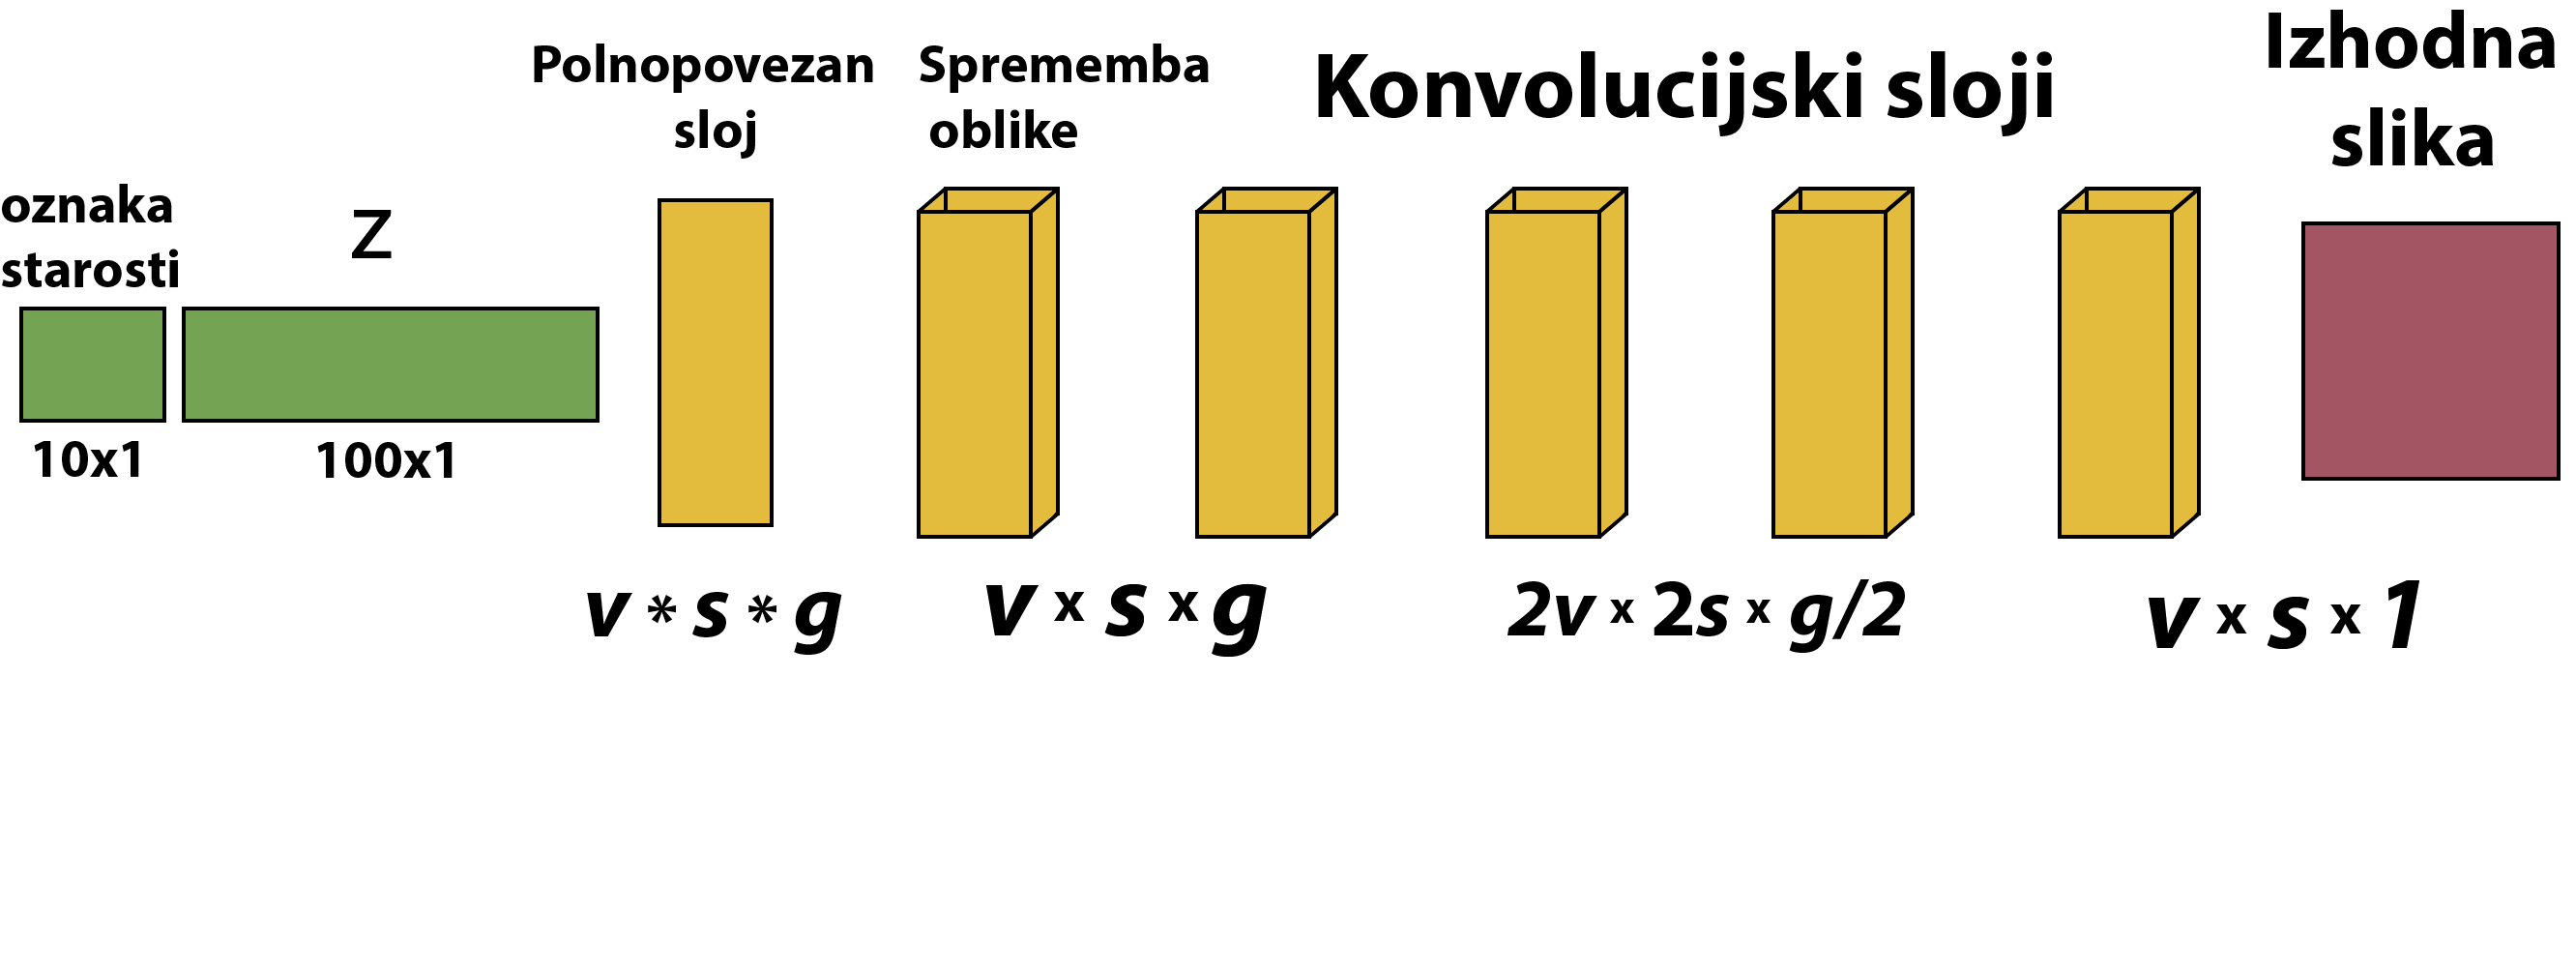
\includegraphics[width=0.85\textwidth]{images/cwgan_generator_a.png}
	\caption[Arhitektura generatorja konvolucijskega CWGAN modela ]{Arhitektura konvolucijskega CWGAN modela}
	\label{fig:cwgan-generator-conv}
\end{figure}

Shema diskriminatorja je podobna. Narejena je tako, da takoj po vhodu sledijo konvolucijski sloji iste dimenzije kot pri generatorju, vendar v obratnem vrstem redu. Za tem pa zravnamo to kar smo dobili s konvolucijami in dodamo polnopovezani sloj velikosti 1. 
Pri generatorju med vsemi sloji uporabljamo tako Dropout kot normalizacijko svežnjev. Aktivacija pri vseh slojih je \textbf{LeakyReLU}, razen v zadnjem konvolucijskem sloju kjer je aktinvacijska funkcija \textbf{tanh}. 
\\
Za diskriminator velja, da med vsemi sloji uporabljamo Dropout ter \textbf{LeakyReLU} aktivacijo za vse sloje, razen za zadnji polnopovezani sloj, kjer se uporablja ReLU aktivacijska funkcija. \\
V sklopu učenja smo uporabljali \textbf{RMSProp} optimizator z nastavljeno hitrostjo učenja kot $0.0005$. Parameter rezanja je bil standardno nastavljen na (-1,1) ter $n_{kritik} =5 $. Velikost batch-a pa smo nastavili na $32$. Začetne uteži so bile inicializirane z vzorčenjem iz normalne porazdelitve. 
Želeli smo mrežo najprej preizkusiti na enostaven način, zato smo se odločili za velikost slike \textbf{64x64} slikovnih točk ter za enokanalne slike. Vsakega od različnih modelov, smo učili za dolžino 20000 svežnjev.
\\
Učenja je potekalo na isti način kot pri implementaciji CGAN modela, kjer smo najprej učili diskriminator, nato pa še skupni model. 
% -- MOVE TO RESULTS 
Pri konvolucijskem modelu, smo dobili dobili rezultate, ki so prikazani na sliki \ref{fig:cwgan-conv-results}. 
\begin{figure}[ht]
  \centering
  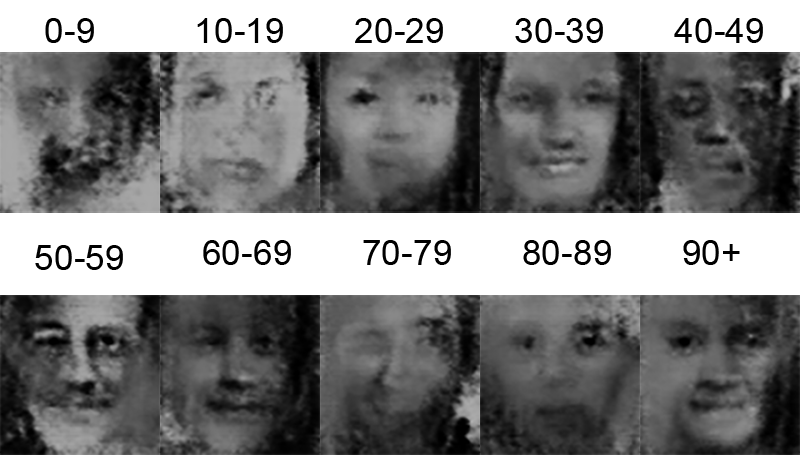
\includegraphics[width=0.5\textwidth]{images/cwgan_conv_results.png}
 \caption[Rezultati učenja CWGAN mreže s konvolucijsko arhitekturo ]{Rezultati učenja CWGAN mreže z konvolucijsko arhitekturo}
  \label{fig:cwgan-conv-results}
\end{figure}
Vidimo, da  je bila naša mreža učena na  učni množici obraznih slik, vendar rezultati niso sprejemljivi, saj so slike zamazane in polne artefaktov. Prav tako so starostni razredi slabo naučeni, saj večina obrazov na slikah na pogled ne pripada pravilni starostni skupini. 

Razlog za slab uspeh učenja lahko najdemo na grafu vrednosti kriterijske funkcije, ki je viden na sliki \ref{fig:cwgan-loss-graph}

\begin{figure}[ht]
  \centering
  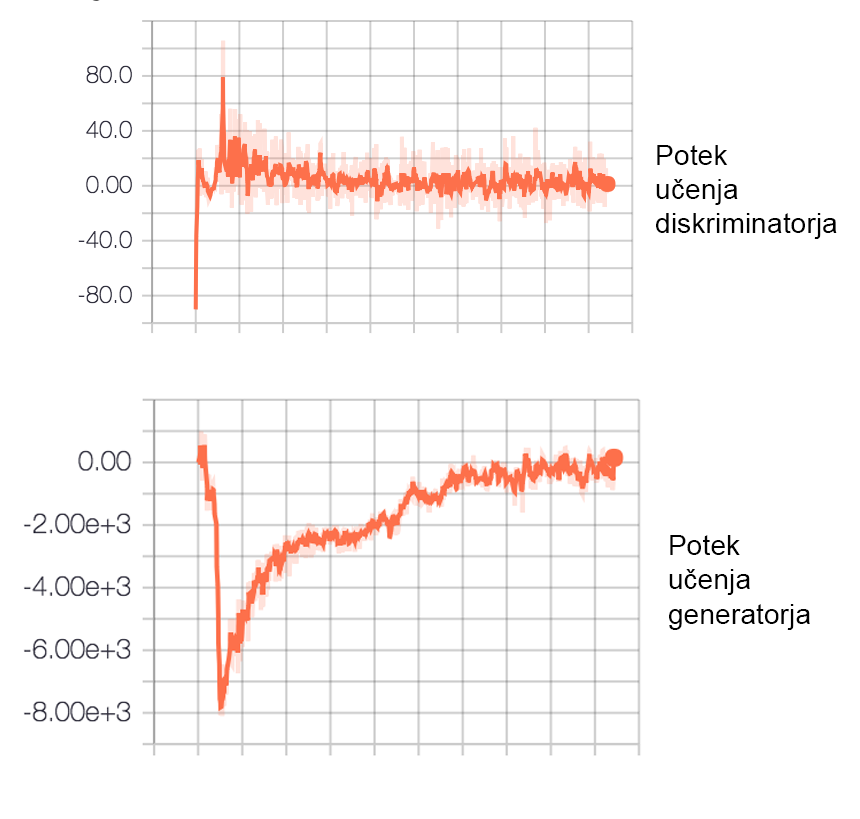
\includegraphics[width=0.5\textwidth]{images/loss_graph_wgan_conv.png}
 \caption[Kriterijska funkcija pri učenju konvolucijskega CWGAN modela ]{Kriterijska funkcija pri učenju konvolucijskega CWGAN modela}
  \label{fig:cwgan-loss-graph}
\end{figure}

Opazimo, da nam diskriminator zelo hitro skonvergira v okolico ničle, vendar se nato tam ne ustali. V času učenja  skače po okolici, kar pomeni, da ne pride do nekih večjih vizualnih izboljšanj. Generator pa  na začetku učenja dobi izrazito negativno vrednost svoje kriterijske funkcije in se nato počasi približuje ničli, a se tudi on tam ne ustali. \\
Da bi izboljšali rezultate, smo poskušali z empiričnim spreminjanjem hiperparametrov (hitrost učenja, $n_{kritik}$, velikost batch-a, število filtrov v konvolucijskih slojih ipd. Prav tako smo poskušali dodati Dropout sloj \cite{srivastava2014dropout} z različnimi parametri, vendar se rezultati niso vidno izboljšali. 
\\
Preizkusili smo tudi uporabo CWGAN arhitekture  s polnopovezanimi sloji, kjer generator s pomočjo zaporednih kaskadnih slojev iz vektorja šuma zgenerira sliko, diskriminator pa samo z uporabo le-teh presodi ali je slika prišla iz množice realnih podatkov ali ne. 
\\Uporabili smo iste parametre za učenje kot pri konvolucijskem modelu, a smo žal dobili rezultate, ki so bili še manj kvalitetni. Po končanem učenju je večino slik vsebovalo le naključni šum, kar je vidno na sliki \ref{fig:cwgan-dense-imgs}. 

\begin{figure}[ht]
  \centering
  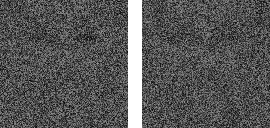
\includegraphics[width=0.2\textwidth]{images/cwgan_dense_noise.png}
 \caption[Vzorec generiranih slik pri CWGAN modelu s polnopovezanimi sloji]{Vzorec generiranih slik pri CWGAN modelu s polnopovezanimi sloji}
  \label{fig:cwgan-dense-imgs}
\end{figure}


Če pogledamo potek učenja na sliki \ref{fig:cwgan-dense-loss-graph},

\begin{figure}[ht]
  \centering
  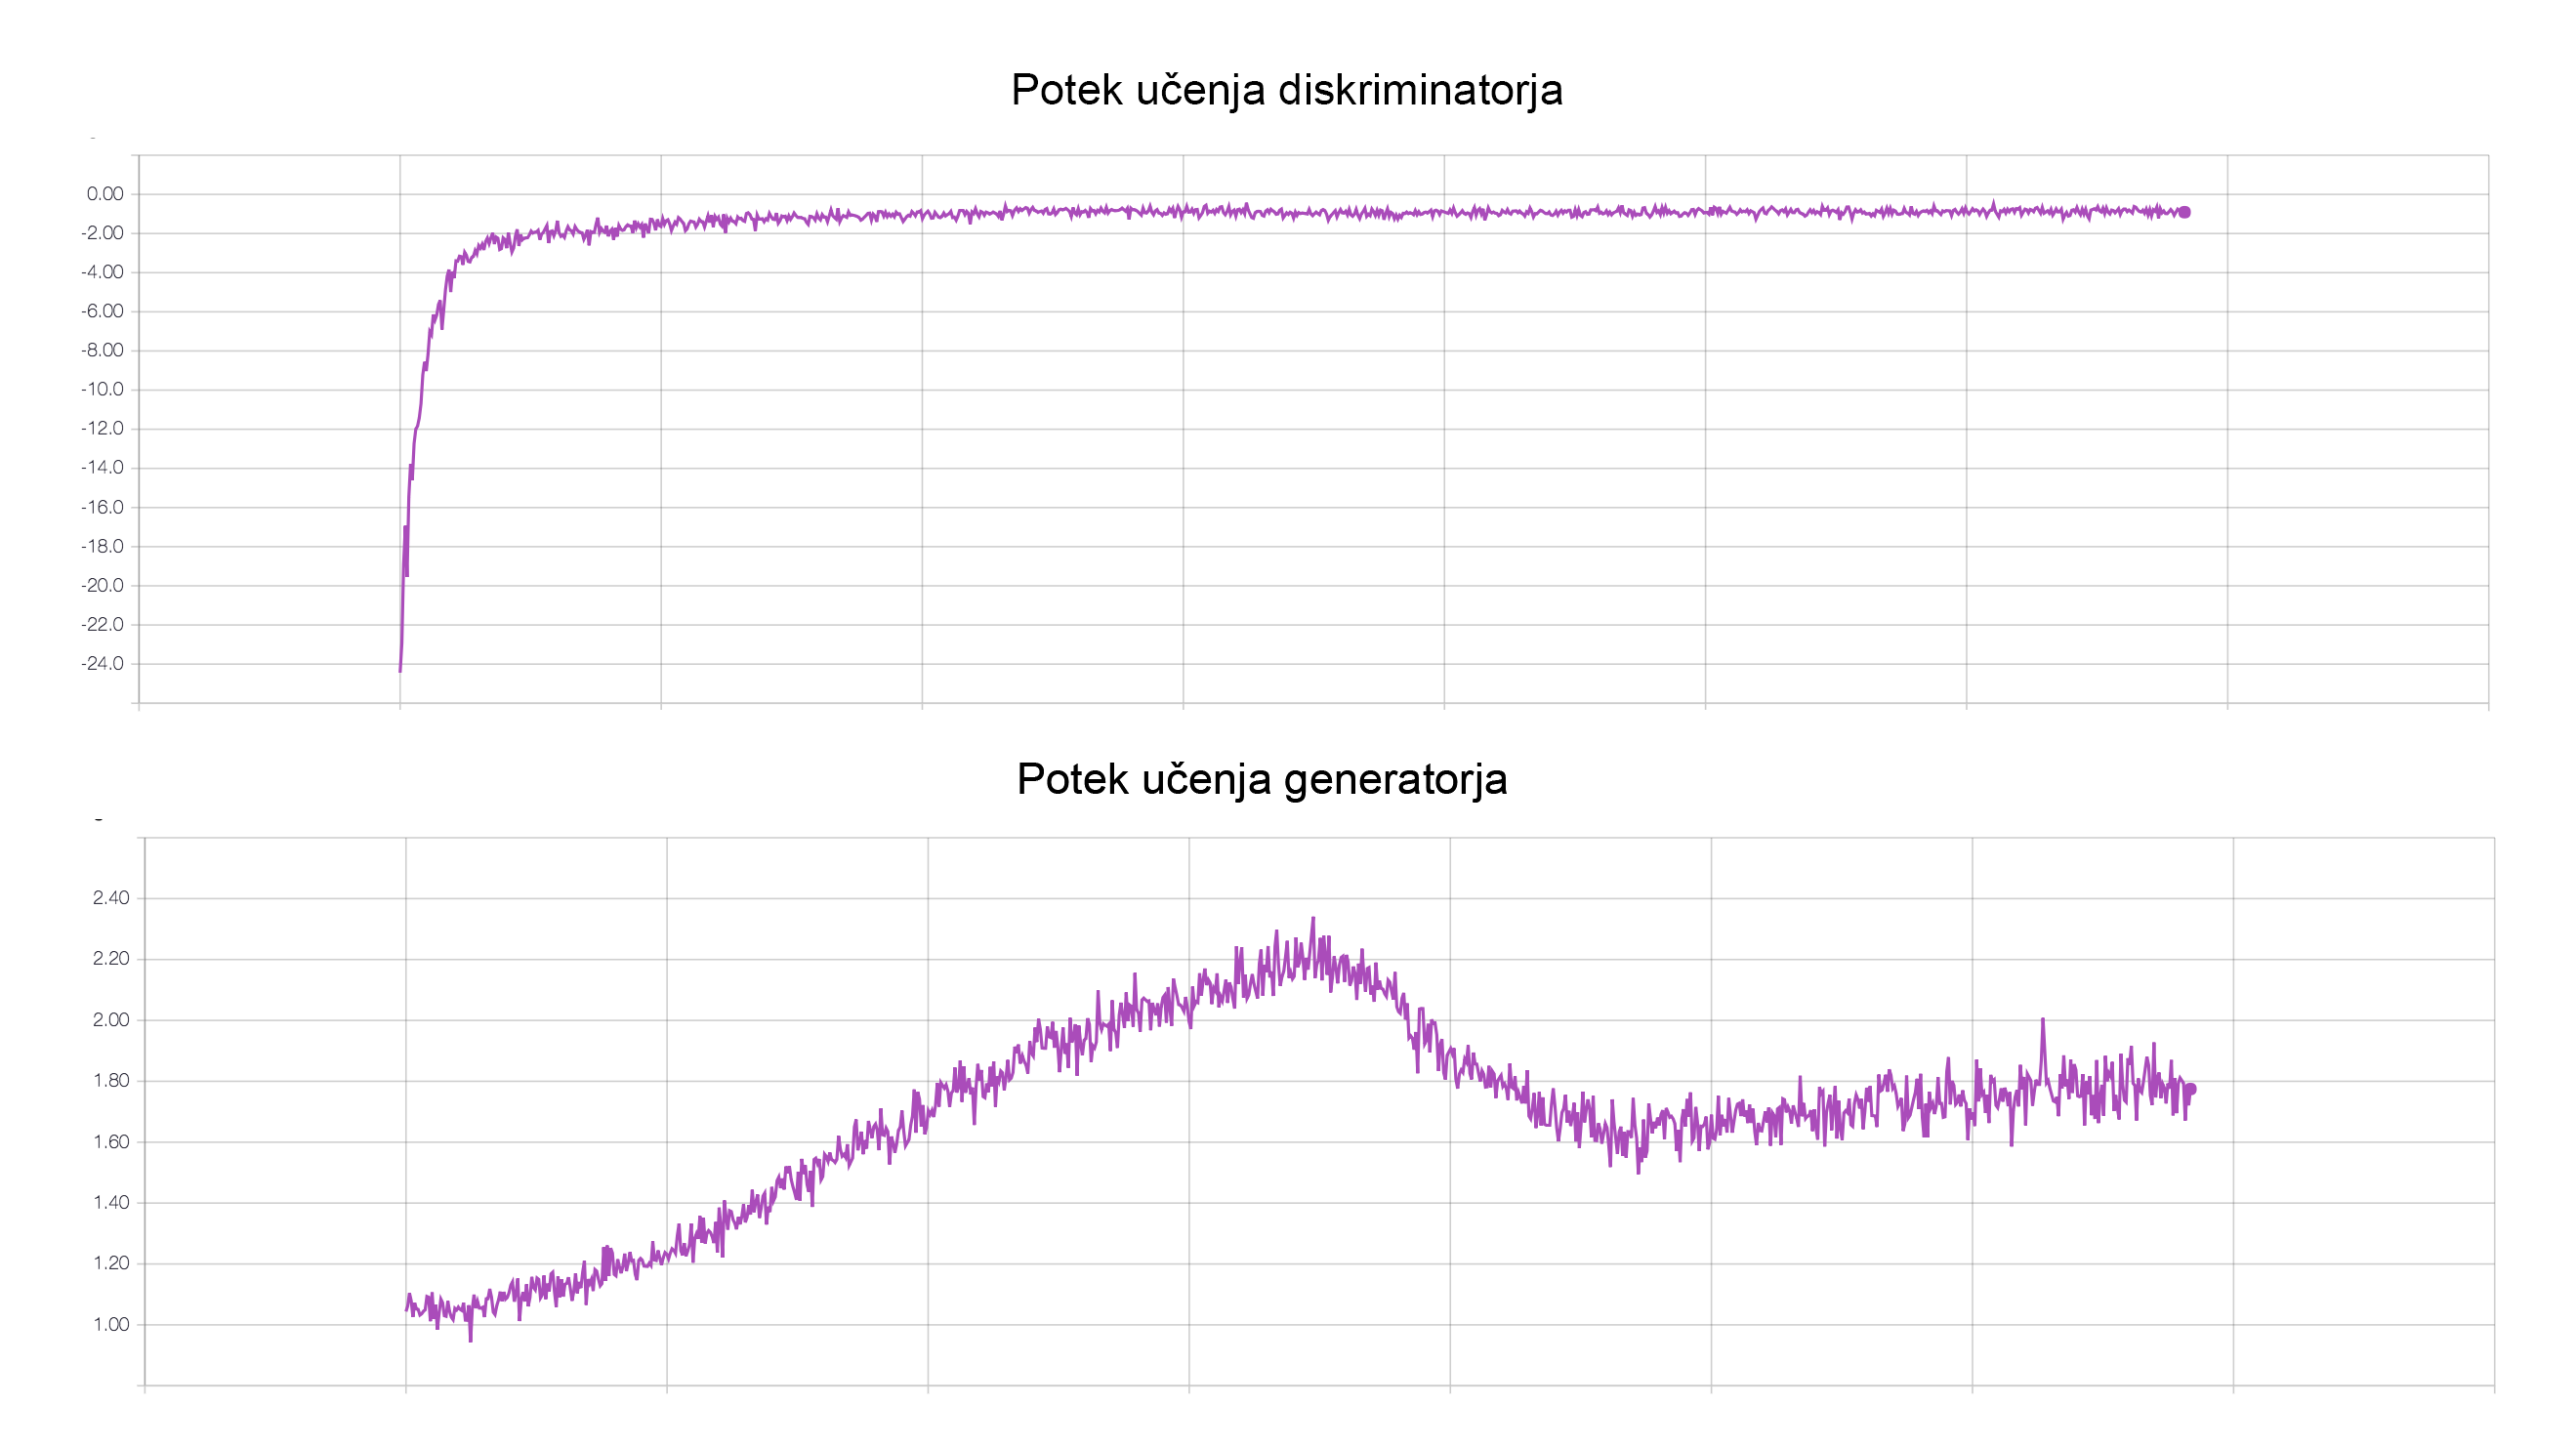
\includegraphics[width=0.8\textwidth]{images/cwgan_dense_loss_graph.png}
 \caption[Kriterijska funkcija pri učenju CWGAN modela s polnopovezanimi sloji ]{Kriterijska funkcija pri učenju CWGAN modela s polnopovezanimi sloji}
  \label{fig:cwgan-dense-loss-graph}
\end{figure}
lahko vidimo da je v tem primeru diskriminator zelo hitro skonvergiral proti optimalni vrednosti 0, medtem ko kriterijska funkcija generatorja ni skonvergirala. To nam lepo prikaže najbolj klasično težavo pri učenju GAN-ov  in sicer neravnovesje v moči med diskriminatorjem  $D$  in generatorjem $G$. V tem primeru je $D$ postal tako dober, da ga $G$, ni znal prelisičiti in medsebojno učenje ni bilo uspešno. Poskusili smo z empiričnim spreminjanjem parametrov, da bi izboljšali rezultate učenja, vendar željenega cilja nismo mogli doseči. 

\section{BiCOGAN}

\subsubsection{Teoretično ozadje}
Klasični GAN modeli nam omogočijo dobiti preslikavo iz prostora šuma $z$ v prostor generiranih podatkov $x$, vendar v procesu očenja žal ne dobimo obratne preslikave $x \mapsto z$, kar je v določenih primerih zaželjeno, saj nam omogoča dobiti kompaktno reprezentacijo naše informacije $x$. 
\\
Rešitev tega problema je model, ki  pogojno generativno nasprotniško mrežo poveže z enkoderjem. ki je zadolžen za določanje inverzne preslikave \cite{jaiswal2017bidirectional}. Velja \cite{donahue2016adversarial}, da v idealnem primeru morata biti $G$ in $E$ inverzna, da lahko prelisičita diskriminator $D$.
\\
V tem primeru primeru se GAN enačba, zapisana v \ref{eq:gan-main} spremeni v
\begin{equation}
 \min_{G}  \max_{D} V(D,G) = \mathbb{E}_{x \sim p_{data}(x)}[\log{D(x,c)}] + \mathbb{E}_{z \sim p_{\tilde{z}}(\tilde{z})}[\log{(1-D(G(\tilde{z},c))}]
\end{equation}

Nas so take mreže zanimale zato, saj bi lahko postopek iz \cite{antipov2017face} poenstovali tako, da bi bila potrebna uporaba samo ene nevronske mreže. Pri omenjenem pristopu, so za določanje preslikave iz prostora slik v prostor latentnih vektorjev, uporabili dodatno nevronsko mrežo, kar pa zahteva izgradnjo dodatnega modela ter učenja, ki je ločen od generiranja slik. 
\\
Želja je bila, da bi z uporabo dvosmernega učenja, hkrati učili tako generator in diskriminator kot tudi enkoder. 
Idejno arhitekturo naše mreže v shematski obliki vidimo na \ref{fig:bicogan-archi}. 
\begin{figure}[ht]
  \centering
  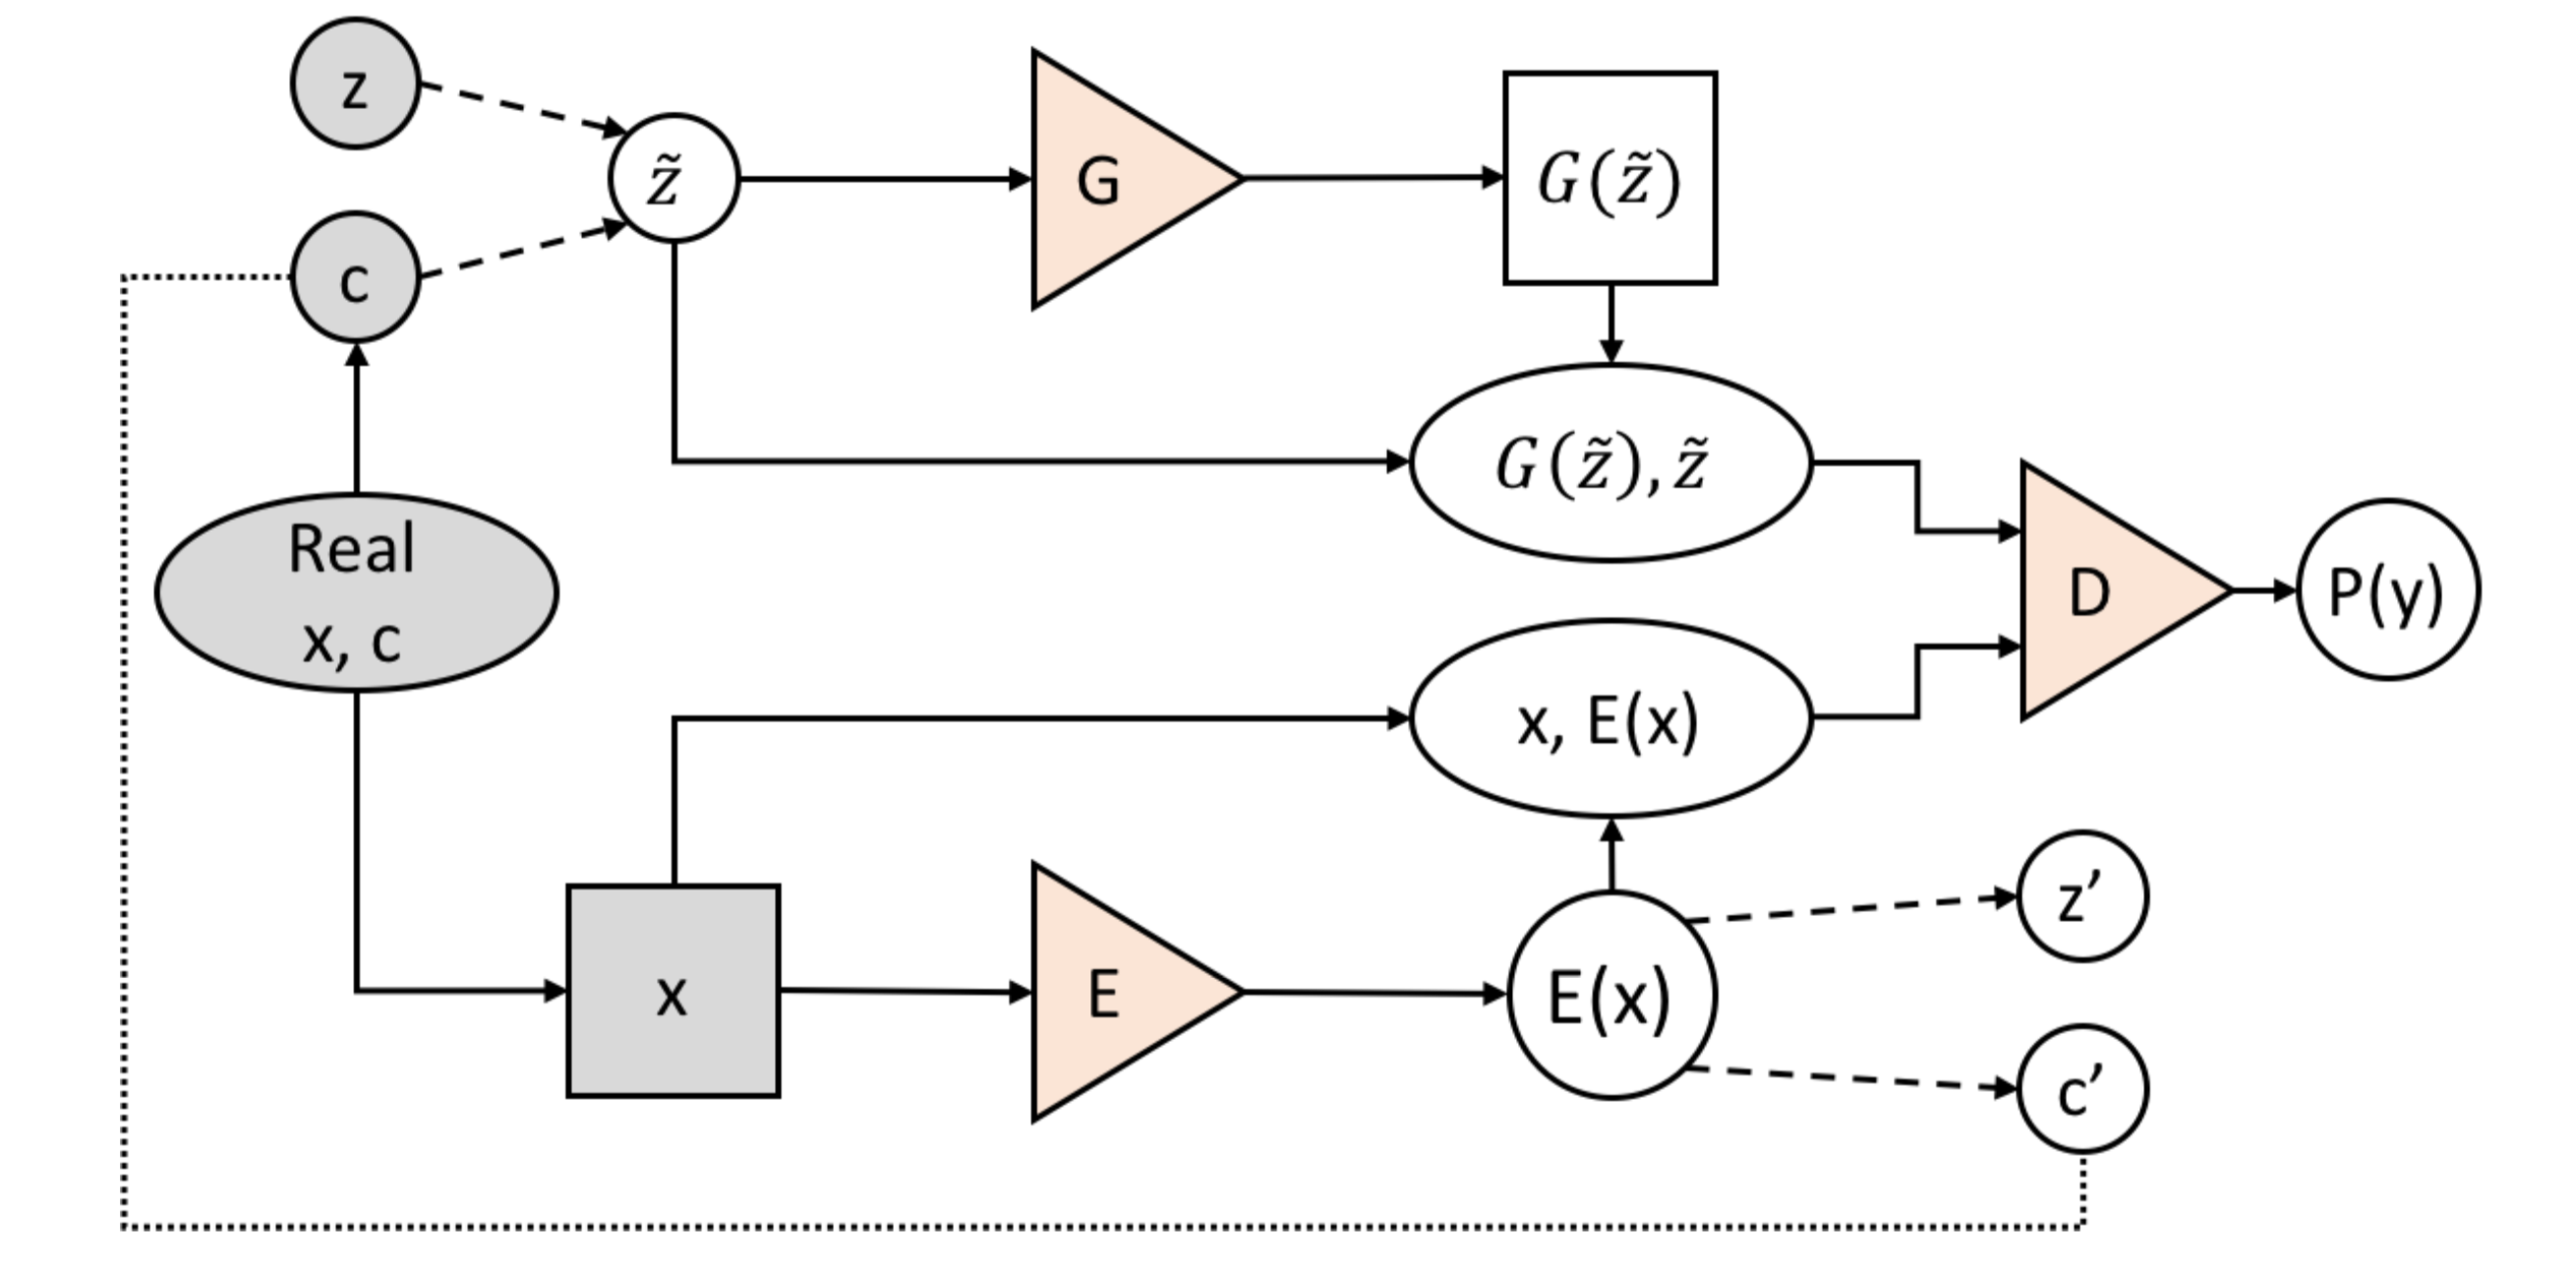
\includegraphics[width=0.7\textwidth]{images/bicogan_shema.png}
 \caption[Idejna zasnova BICOGAN arhitekture, vir: \cite{jaiswal2017bidirectional} ]{Idejna zasnova BICOGAN arhitekture.Vir:\cite{jaiswal2017bidirectional} }
  \label{fig:bicogan-archi}
\end{figure}

Če se nanašamo na oznake, definirane v poglavju o navadnih GAN mrežah, 
potem formalno rečemo, da se generator nauči preslikavo $G(\tilde{z},\theta_G)$ iz porazdelitvne $p_{\tilde{z}}$, kjer je $\tilde{z} = [z \text{ } c]$ v 
porazdelitev $p_G$, kjer je glavni cilj da se $p_G$ in $p_{data}$ čim manj razlikujeta.  Naloga enkoderja $E(x;\theta_E)$ je da slika iz $p_{data}$ v $p_{E}$, kjer želimo da je $p_E$ čim bližje $p_{\tilde{z}}$. Diskriminator  se odloča o avtentičnosti vzorca glede na  $D(\tilde{z},G(\tilde{z});\theta_D)$ in $D(E(x),x;\theta_D)$. 
\\ V splošnem primeru BICOGAN modela  se mora enkoder  naučiti inverzni preslikavo iz $x$ v $z$ \textbf{in} $c$. Ker pa  je to v našem primeru nepotrebno, smo naš model spremenili tako, da je informacija o oznaki $c$ enkoderju vedno podana. 
\subsubsection{Eksperimentalni rezultati}

Poizkusili smo z implementacijo BICOGAN modela v orodju Keras. Kot najenostavnejšo obliko smo za vse tri notranje mreže (diskriminator, generator, enkoder) uporabili polnopovezano arhitekturo. Rezultati, ki smo jih dobili so prikazali solidne vizualne rezultate s strani generatorja,  kar vidimo na sliki \ref{fig:bicogan-generated}. Težave so nastale pri enkoderju. Ni nam uspelo, da bi se enkoder pravilno naučil preslikave iz $x$ v $z$. Veljati bi namreč moralo, $G(E(x)) \sim  x$, vendar je iz generiranih slik očitno, da to ni uspelo. Na sliki \ref{fig:bicogan-encoder} na levem delu vidimo naš $x$ in na desnem vidimo $G(E(x))$. V idealnem primeru, bi bili sliki identični oz. zelo podobni, vendar vidimo da je razlika prevelika.  

\begin{figure}[ht]
  \centering
  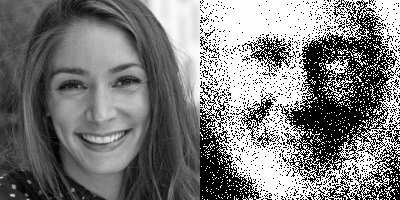
\includegraphics[width=0.7\textwidth]{images/bicogan_encoder.png}
 \caption[Leva slika predstavlja naš $x$, desna pa naš $G(E(X))$ ]{Leva slika predstavlja naš $x$, desna pa naš $G(E(X))$ } 
  \label{fig:bicogan-encoder}
\end{figure}

Še ena od težav je, da arhitektura s polnopovezanimi sloji generira slike, ki so polne šume in zatorej precej različne od realnih podatkov. 

\begin{figure}[ht]
  \centering
  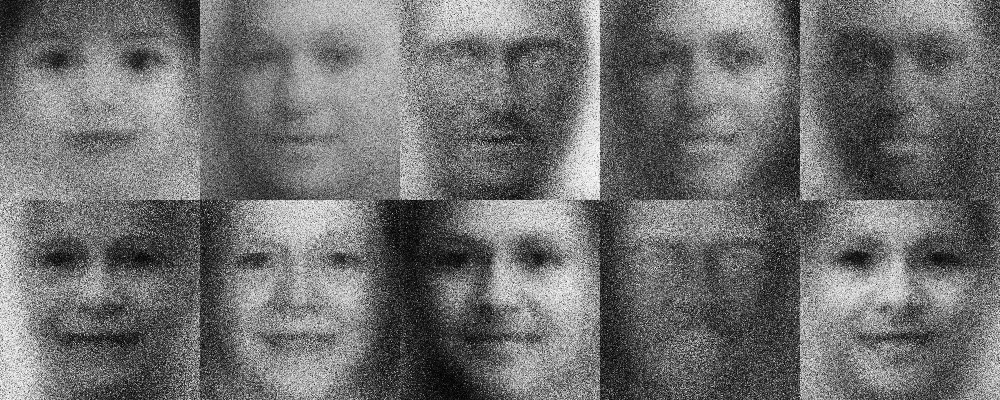
\includegraphics[width=0.7\textwidth]{images/bicogan_generated_imgs.png}
 \caption[Obrazi ustvarjeni s pomočjo BICOGAN mreže ]{Obrazi ustvarjeni s pomočjo BICOGAN mreže} 
  \label{fig:bicogan-generated}
\end{figure}

Težave, ki se pojavljalo pri učenju BICOGAN modelov, so iste narave kot pri učenju klasičnih GAN mrež, vendar so zaradi narave mreže še bolj potencirane. Ker smo sedaj v mrežo vklučili še enkoder, postane naša mreža še bolj občutljiva na nastavljanje hiperparametrov. Velja namreč, da zelo hitro pride do neravnovesja med tremi glavnimi komponentami mreže. V takem primeru skozi nasprotniško učenje težko dosežemo optimalno rešitev, saj ena od mrež prevlada nad ostalimi.  Kot vidimo na grafih  \ref{fig:bicogan-los} kriterijske funkcije   generatorja in diskriminatorja vidimo do konvergence ne pride, opazimo pa, da sta si grafa približno zrcalna preko x-osi. To nam potrjuje nasprotniško učenje teh dveh mrež. Kadar ena od mrež postane močnejša, druga postane šibkejša.  
\begin{figure}[ht]
  \centering
  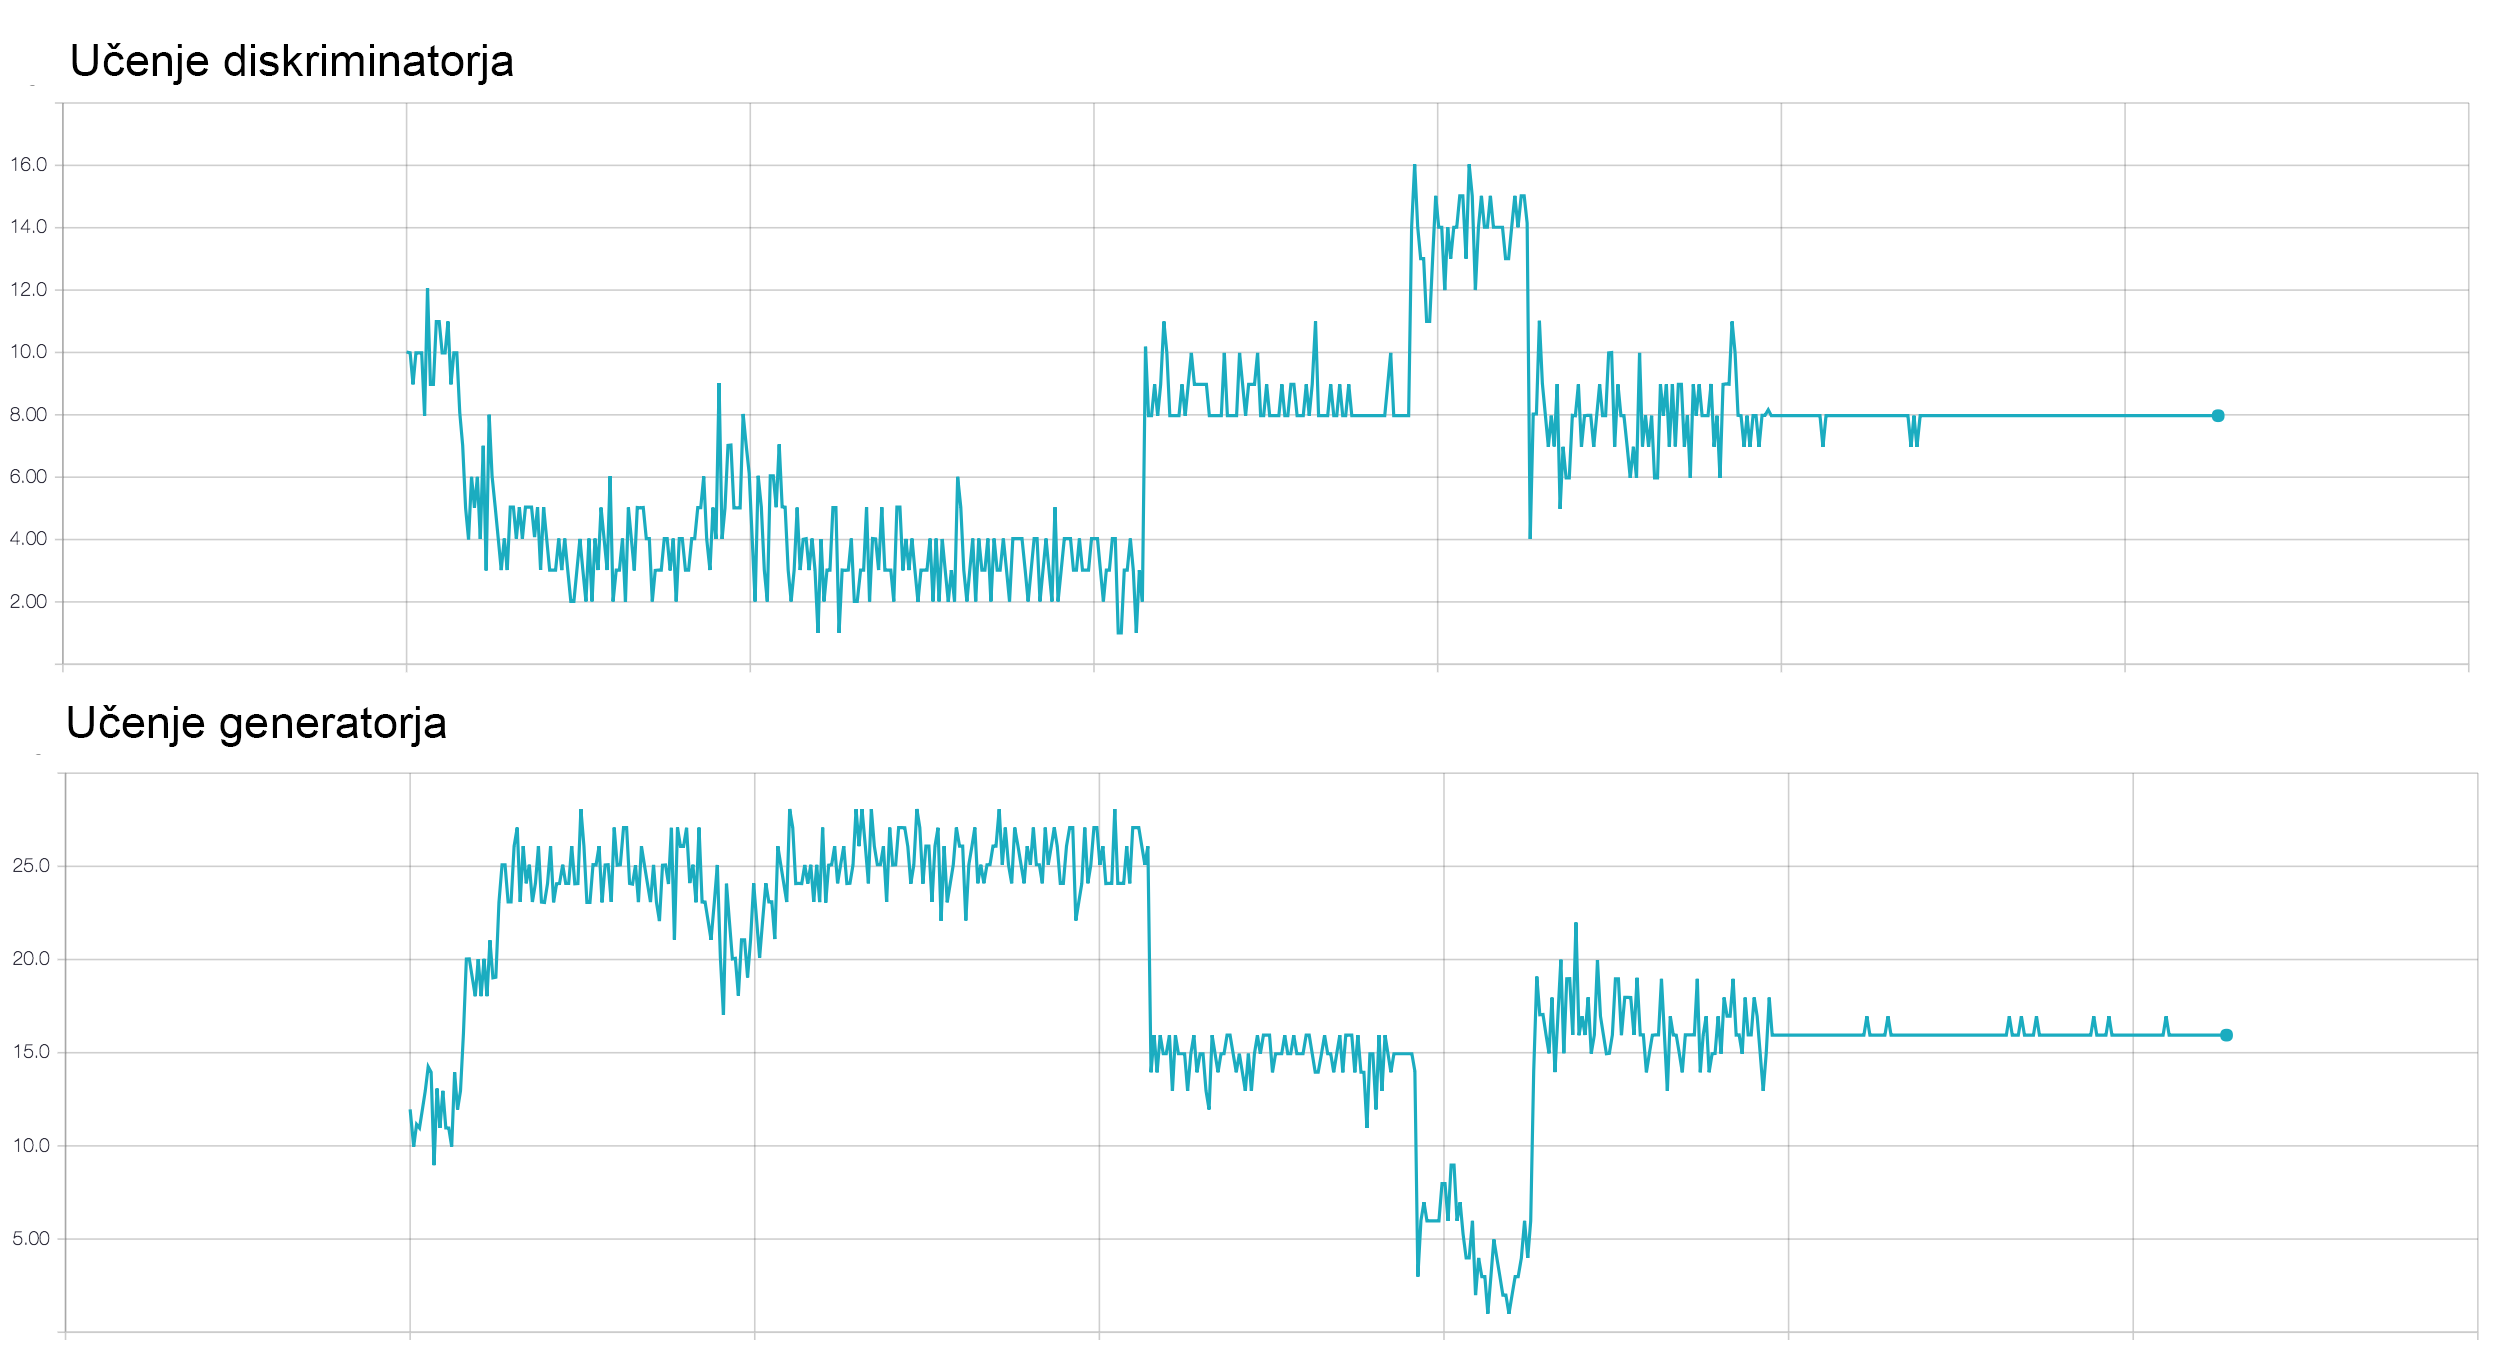
\includegraphics[width=0.7\textwidth]{images/bicogan_training.png}
 \caption[Učenje diskriminatorja in generatorja BICOGAN mreže ]{Učenje diskriminatorja in generatorja BICOGAN mreže} 
  \label{fig:bicogan-los}
\end{figure}

\section{Variacijski autoenkoder}
Zaradi nezadovoljivih rezultatov dobljenih s pomočjo različnih inačic generativnih nasprotniških mrež smo se odločili za preizkus metod, ki uporabljajo variacijske autoenkoderje. 
Najprej smo želeli preizkusiti VAE kot generativni model, ki je sposoben ustvariti realne slike obrazov različnih starosti. 
\subsection{Enostavna polnopovezana arhitektura}
Zgradili smo najenostavnejšo arhitekturo sestavljeno iz polnopovezanih slojev, ki je predstavljena na sliki \ref{fig:vae-architecture}. 

\begin{figure}[ht]
  \centering
  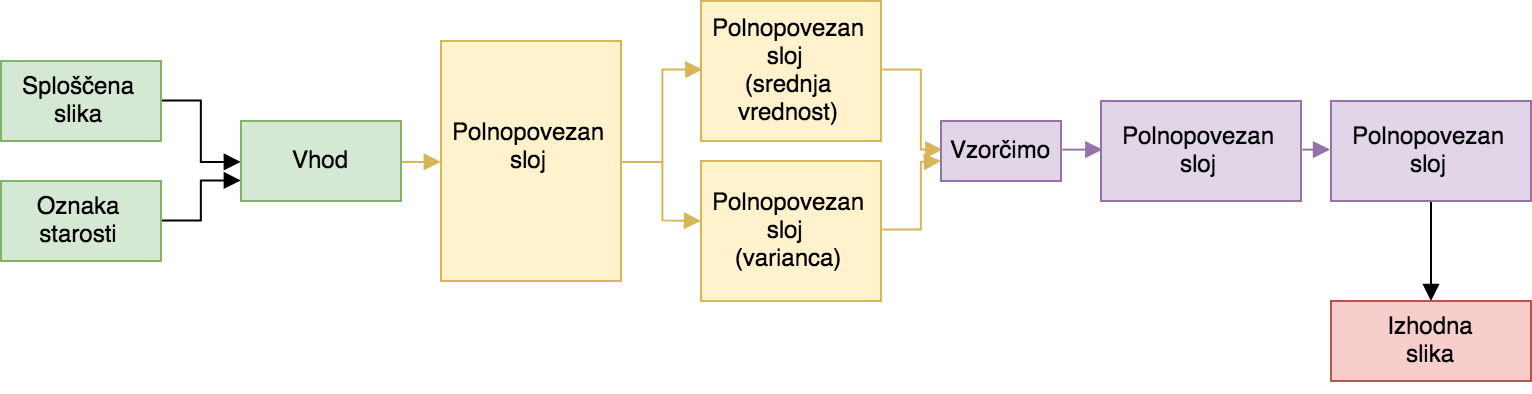
\includegraphics[width=0.85\textwidth]{images/vae_shema.png}
 \caption[Najenostavnejša arhitektura variacijskega autoenkoderja ]{Najenostavnejša arhitektura variacijskega autoenkoderja} 
  \label{fig:vae-architecture}
\end{figure}

Z zeleno barvo so označeni vhodni sloji, z rumeno barvo je označen del mreže, ki pripada enkoderju $E$, z vijolično barvo pa tisti del, ki pripada enkoderju $D$. Kot izhodni podatek, označen z rdečo, dobimo sliko, ki jo je enkoder ustvaril iz latentnega vektorja, ki je bil vzorčen. 
\\
Glavna ideja variacijskega autoenkoderja je vzorčenje latentnega vektorja iz dveh polnopovezanih slojev, katrih nevroni predstavljajo srednjo vrednost in varianco. Kadar želimo dobiti latentni vektor, vzorčimo iz sloja standardnih deviacij  in mu prištejemo srednjo vrednost.
Vrednost vzorčenja $v$ matematično zapišemo kot 

\begin{equation}
	v = \mu + e^{\sigma}\epsilon
\end{equation}

kjer $\epsilon$ predstavlja vzorčeno vrednost iz naravne porazdelitve s standardno deviacijo $\epsilon_{\text{std}}$. To lahko nastavljamo kot parameter našega modela. 
 
 Velikosti vseh notranjih slojev so prepuščene izbiri in so določene glede na vhodne podatke in empirično preizkušanje. 
 \\
 V našem primeru smo nastavili dimenzijo prvega polnopovezanega sloja v $E$ na 512 nevronov, medtem ko smo velikost slojev srednjih vrednosti in variance nastavili na 100. Sloj vzorčenja mora tudi imeti dimenzijo 100. Prvi polnopovezan sloj $D$ je dimenzije 512 medtem, ko mora drugi polnopovezan sloj imeti dimenzijo enako velikosti izhodne slike. 
 \\ 
 Pri $E$ uporabljamo \textit{ReLU} aktivacijsko funkcijo za polnopovezan sloj, ter \textit{linearno} aktivacijo za sloj s srednjo vrednostjo in standardno variacijo.  Podobno velja, da je ima prvi sloj dekoderja \textit{ReLU} aktivacijo, zadnji pa \textit{sigmoid}. 
 \\
 Pri variacijskem autoenkoderju imamo še en parameter, ki bistveno vpliva na potek učenja in sicer razmerje med \textbf{rekonstrukcijsko napako} in \textbf{KL divergenco}, katerih seštevek predstavlja kriterijsko funkcijo modela. Absolutna vrednost teh dveh količin je precej različna, zato ju moramo znormalizirati. Opazili smo, da razmerje med tema dvema količinama močno spremeni nape rezultate. V primeru kadar prevlada rekonstrukcijska napaka dobimo precej dobre rekonstrukcije originalnega vhoda, vendar staranje ne deluje. Kadar pa prevlada KL divergenca dobimo zelo povprečne obraze vseh starostnih skupin, kar nam za naš namen ne koristi. Ko pomislimo o definiciji KL divergence, ima to smisel, saj velja, da je $KL divergenca$ mera razdalje med dvema verjetnostnima porazdelitvama. Tukaj je ena od porazdelitev tista, ki se jo učimo v želji, da bi lahko generirali slike, ki so podobne vhodnem. Druga pa predstavlja normalno porazdelitev na prostoru vseh obrazov. Kadar KL divergenca prevlada, je torej zelo blizu povprečnemu obrazu in identiteta osebe se v procesu izgubi.
 \\ 

 Kot pravilo palca smo najprej normalizirali rekonstrukcijsko napaka z velikostjo vhodnih podatkov. Naprimer, če smo imeli velikost vhodne slike 128x128 slikovnih točk in enokanalno sliko smo vrednost delili z 16384. KL divergenco pa smo delili z velikostjo latentnega prostora.
 Dodali smo še eno utež, ki je delovala neodvisno od dimenzije slike in smo jo spreminjali, da bi dobili najboljše razmerje med obema vrednostima. Empirično smo ugotovili, da smo dobili najboljše rezultate kadar smo dodatno pomnožili KL divergenco s faktorjem okoli 0.1.
 \\ 
 Spreminjanje $\epsilon_{\text{std}}$ nam, glede na izkušnje iz poizkušanja, naredi podobno kot zgoraj opisano razmerje. Z zmanjšanjem parametra, dosežemo, da generiranje slike ohranijo večjo podobnost vhodni slike in manjšo podobnost povprečju celega razredu. Zaradi narave našega problema - želimo ohraniti identiteto ob prilaganju povprečju razreda (starosti) je težko določiti optimalno mejo.,  
 
 Dobljeni rezultati so predstavljeni v poglavju Rezultati, vendar velja omeniti, da smo dosegli precej boljšo vizualno kvaliteto kot pri generativnih nasprotniških mrežah. Ker je predstavljena arhitektura najbolj osnovna možna, smo se odločili, da bomo poskusili z implementacijo konvolucijskega variacijskega autoenkoderja, ki je bolj primeren za delovanje na slikah.  
 
 \subsection{Konvolucijska arhitektura}
  Odločili smo se za konvolucijsko arhitekturo s štirimi zaporednimi konvolucijskimi sloji v enkoderju ter analogno arhitekturo v dekoderju. 
  Na sliki \ref{fig:vae-encoder-conv} vidimo arhitetekturo enkoderja, medtem ko na \ref{fig:vae-decoder-conv} vidimo arhitekturo dekoderja. 
  \begin{figure}[ht]
  	\centering
  	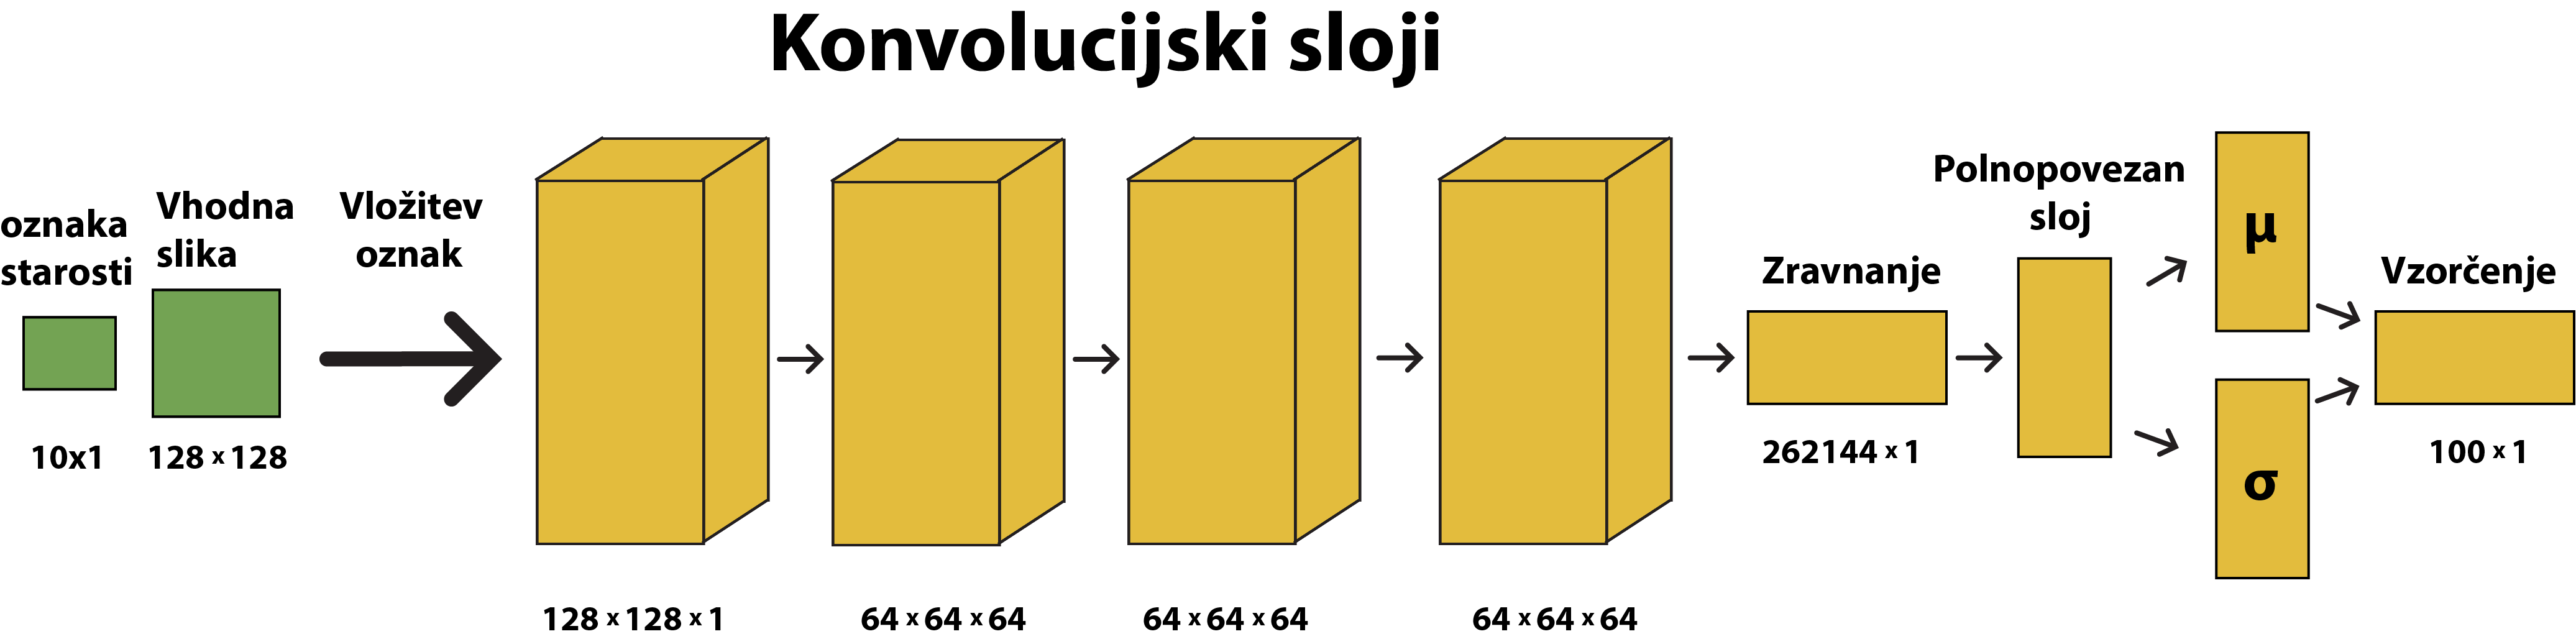
\includegraphics[width=1.0\textwidth]{images/vae_classic_conv_encoder.png}
  	\caption[Arhitektura enkoderja pri konvolucijskem VAE modelu ]{Arhitektura enkoderja pri konvolucijskem VAE modelu } 
  	\label{fig:vae-encoder-conv}
  \end{figure}

Velja omeniti, da so dimenzije konvolucijskih slojev odvisne od velikosti vhodnih podatkov. Shema modela je narejena pri predpostavki, da je velikost vhodne slike 128x128 slikovnih točk, ter da generiramo latentni vektor velikost 100. Predvsem velikost latentnega vektorja lahko močno vpliva na kvaliteto generiranih slik. 

   \begin{figure}[ht]
   	\centering
   	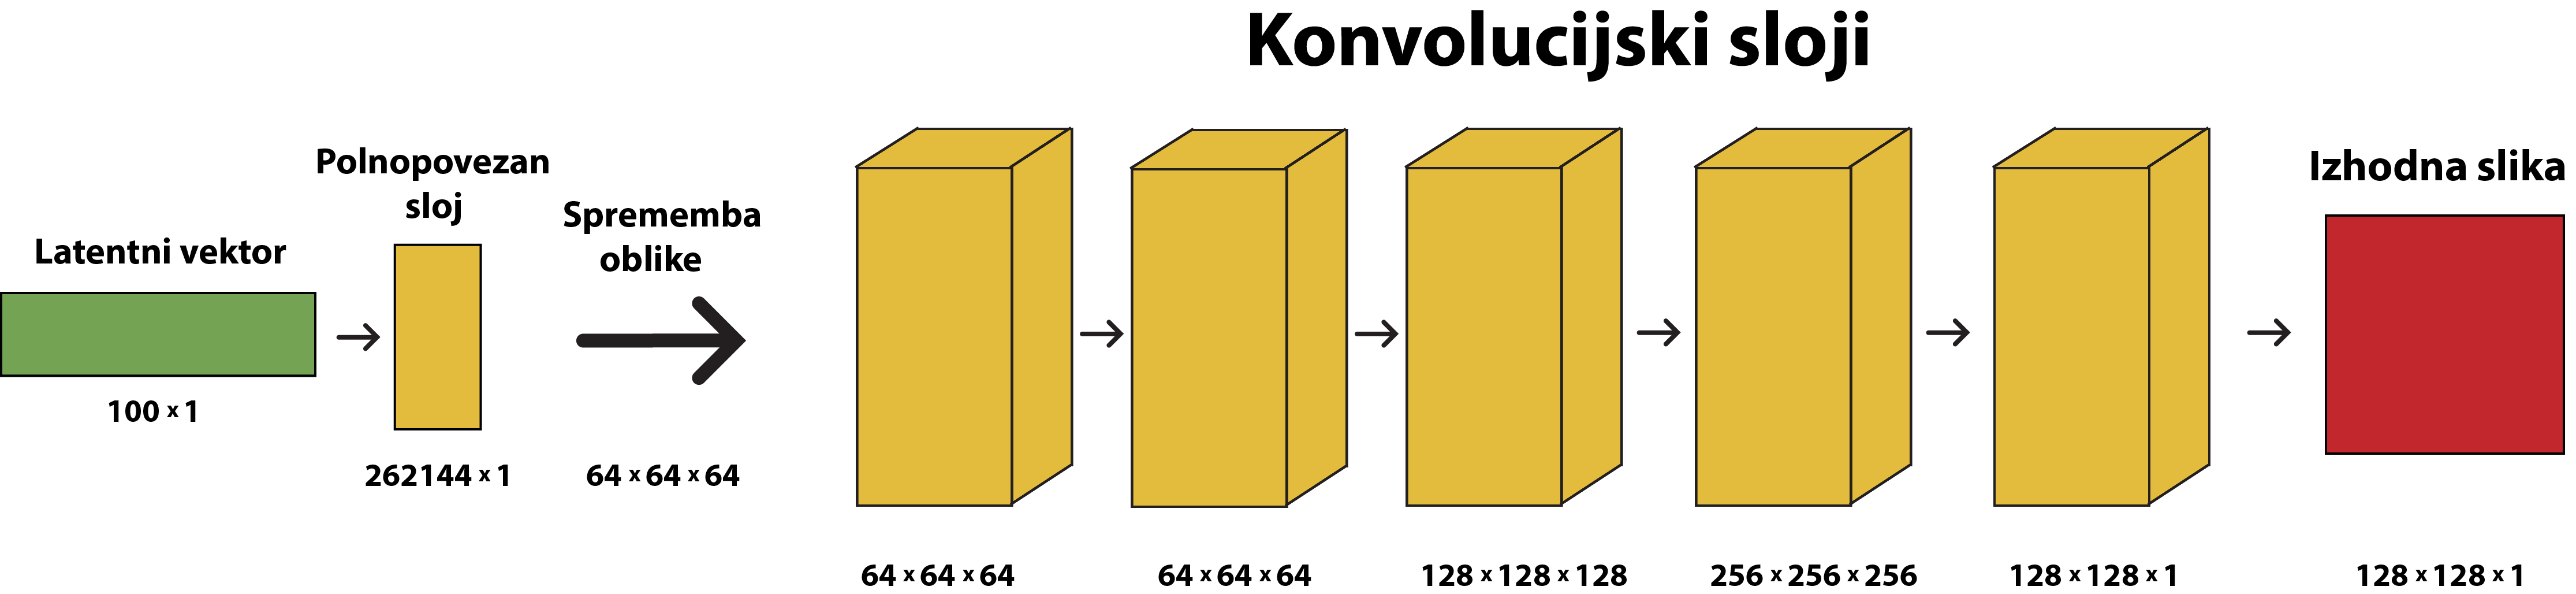
\includegraphics[width=1.0\textwidth]{images/vae_classic_conv_decoder.png}
   	\caption[Arhitektura dekoderja pri konvolucijskem VAE modelu ]{Arhitektura dekoderja pri konvolucijskem VAE modelu } 
   	\label{fig:vae-decoder-conv}
   \end{figure}
   
Poleg parametrov, ki smo jih definirali pri polnopvoezani arhitekturi, imamo pri konvolucijskem modelu dodatne parametre, ki vplivajo na končni rezultat. Prvi je število filtrov, ki določa koliko filtrov se naša mreža uči v v vsakem od slojev. Kot vidimo na sliki \ref{fig:vae-decoder-conv} in \ref{fig:vae-encoder-conv}, je standardno število filtrov, ki smo ga nastavili 64. V propagaciji skozi dekoder, se število filtrov spreminja skupaj z dimenzijo. Poleg tega pa je pomembno določiti tudi velikost jedra konvolucije. V enkoderju imamo velikost jedra 2 v dekoderju pa 3. V vseh slojih slojih uporabljamo \textit{ReLU} aktivacijo, razen v zadnjem sloju dekoderja, kjer se kot aktivacija uporablja \textit{sigmoid}. Optimizator smo nastavili na \textsc{RMSProp}. 


\subsection{Konvolucijska arhitektura s kritikim identitete}
V sklopu preizkušanja modelov, smo naleteli na težavo, da so bile generirane slike preveč povprečne. Poizkušali smo spreminjati različne parametre našega modela, vendar nam večjih izboljšav ni uspelo doseči. To težavo smo želeli odpraviti z implementacijo variacijskega autoenkoderje, kateremu bi dodali kritika, ki bi bil zadolžen za premikanje mreže v smeri ohranjanja identitete. 
Naš idejni model je predstavljen na \ref{fig:vae_id_shema},
\begin{figure}[ht]
\centering
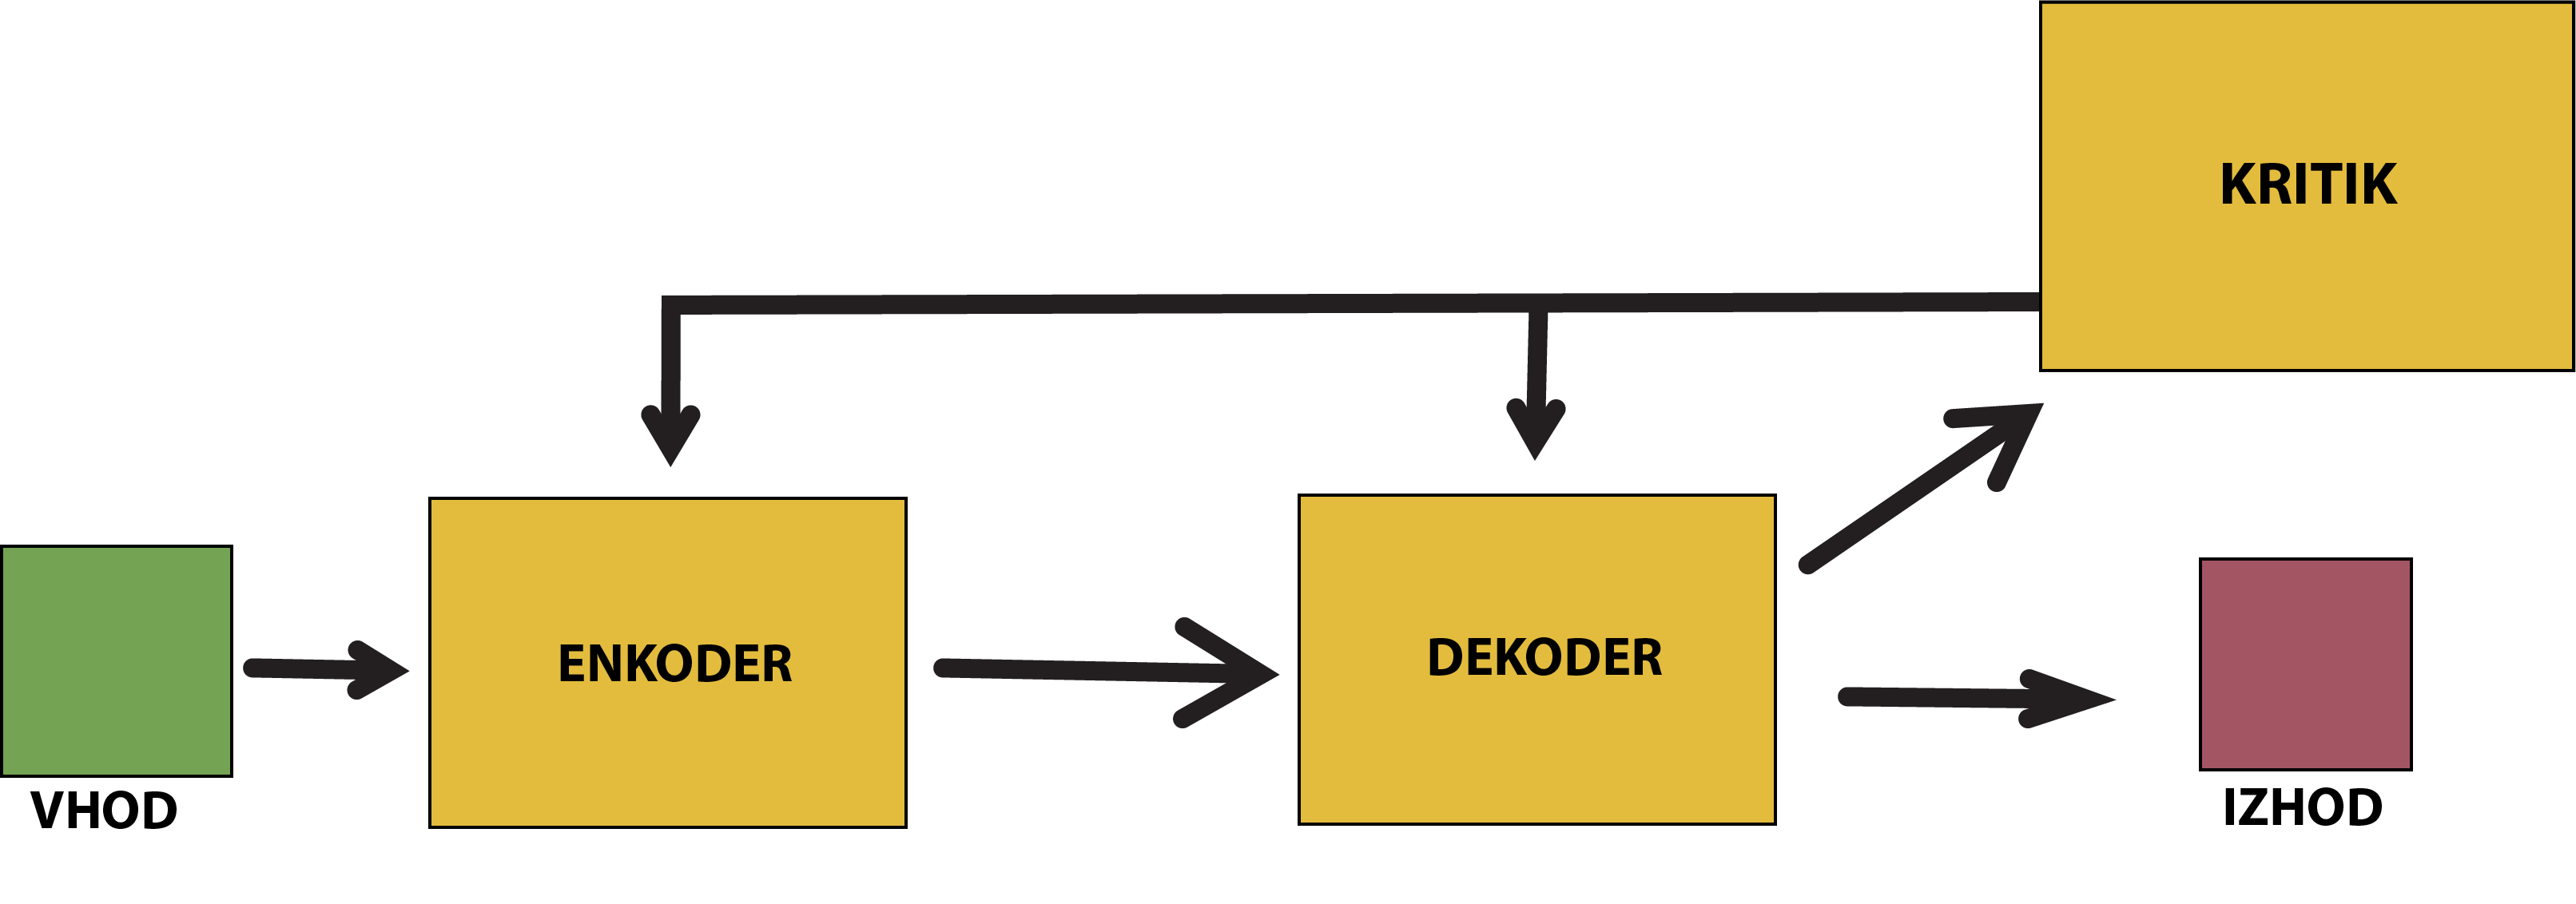
\includegraphics[width=0.8\linewidth]{figures/images/vae_id_shema}
\caption{Idejna zasnova variacijskega autoenkoderja s kritikom identitete.}
\label{fig:vae_id_shema}
\end{figure}
kjer lahko vidimo, da je kritik povezan z izhodom in usmerja celotno mrežo (tako enkoder kot dekoder) v to, da bi generirala boljše slike. Kritik deluje tako, da sprejme vhodne sliko ter generirano sliko ter nam vrne mero podobnosti med identitetami oseb na teh slikah.  Želimo torej dodatni dodaten kriterij h kriterijski funkcijami, ki bi poskrbel za podobnost identitet. Želimo torej minimizirati naslednjo vsoto 
$\mathcal{L} = \lambda_1 \mathcal{L}_{KL} + \lambda_2 \mathcal{L}_{\text{rekon}} + \lambda_3 \mathcal{L}_{id}$, kjer lahko vsakega od členov celotne kriterijske funkcije pomnožimo s skalarjem in s tem reguliramo njegovo pomembnost. 
\\
Zelo je pomembna izbira kritika identitete. Najprej smo poskušali uprabiti prednaučeni model Squeezenet mreže \cite{iandola2016squeezenet}, ki je bila učena na obrazih. Arhitekturo squeezenet mreže vidimo na sliki \ref{fig:squ_architecture}.

\bibliographystyle{elsarticle-num}
\begin{figure}[th]
	\centering
	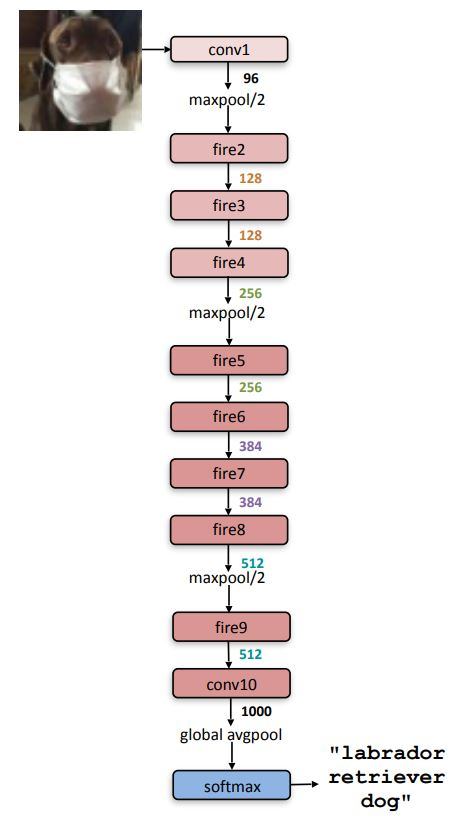
\includegraphics[width=0.4\linewidth]{figures/images/squ_architecture}
	\caption{Arhitektura squeezenet mreže. Vir: \cite{iandola2016squeezenet}}
	\label{fig:squ_architecture}
\end{figure}

Posebnost te mreže so t.i. fire sloji, ki so sestavljenih iz treh konvolucij, ki vhod stisnejo in nato ponovno razširijo. Ta mreža je dosegala zelo dobre rezultate kot klasifikacijski model, največja prednost pa je fizična velikost modela. Zaradi omejitev strojne opreme, natančneje spomina na grafični kartici je to lahko zelo priročno, saj se ob večjih modelih hitro lahko zgodi, da presežemo omejitve strojne opreme. V takem primeru moramo praviloma zmanjševati velikost svežnjev pri učenju, kar nam praviloma podaljša učni čas. 
\\
Mreža je bila predhodno učena na množici obraznih slik z namenom klasifikacije oseb. Uporabljala se je baza \cite{parkhi2015deep}.   Za razliko od naše podatkovne baze, slike v tej bazi  niso bile poravnane ter obrezane, da bi upoštevale striktno samo obrazni del, brez ostalih faktorjev kot so obleka, lase ipd.  Pred preizkušanjem nismo vedeli, ali bo to predstavljalo težavo, ker nam ni bilo znano koliko se prednaučena mreža zanaša na značilke pridobljene iz konteksta slike. 
\\ Mreža je narejena za klasifikacijo, torej nam ob podani vhodni sliki vrne vektor verjetnosti, katera oseba je na tej sliki. Vsak element tega vektorja predstavlja eno od oseb iz učne množice. Ker je podatkovna baza ki jo uporabljamo za staranje različna in posledično identitete oseb drugačne kot v squeezenet mreži, moramo implementacijo malenkost spremeniti. Namesto da vračamo verjetnosti, mrežo odrežemo pred zadnjim slojem in vračamo vektor značilk, dolžine 2048,  ki naj opisuje identiteto osebe v reprezentaciji, ki se jo je naučilo nevronska mreža. 
\\
Kadar želimo primerjati podobnost dveh slik obrazov, lahko uporabimo kosinusno razdaljo, ki je definirana kot 

\begin{equation}
	\text{podobnost} = \frac{\textbf{A} \cdot \textbf{B}}{||\textbf{A}|| \cdot || \textbf{B} ||  } = \frac{\sum_{i=1}^n A_iB_i}{\sqrt{\sum_{i=1}^n A_i^2}\sqrt{\sum_{i=1}^{n}B_i^2}}
\end{equation}
kjer sta $\textbf{A}$ in $\textbf{B}$ vektorja, ki ju želimo primerjati in $A_i,B_i$ njune komponente. Kot je očitno iz enačbe, se formula precej poenostavi, če sta vektorja normalizirana. V takem primeru moramo za mero podobnosti izračunati le skalarni produkt med tema dvema vektorjema.  Mera se se giblje med -1 in 1, kjer 1 označuje največjo podobnost in -1 največjo različnost.
\\

Za implementacijo našega modela smo morali najprej za vse slike v naši učni množici izračunati vektor značilk, da smo lahko primerjali generirano sliko lahko primerjali z obrazom, ki je bil podan na vhod.  
Končni model je torej na vhod prejel sliko osebe, njeno starost ter vektor predhodno izračunanih značilk identitete, na izhod pa je vrnil ustvarjeno sliko ter vektor pripadajočih značilk. Ker je ta vektor potreben za izračunanje kriterijske funkcije govorimo o t.i. obojestranskem (end-to-end) postopku. 
Velja omeniti, da sta bila enkoder in dekoder definirana s konvolucijsko arhitekturo, kot je opisana v prejšnjem podpoglavju. Tudi uporabljeni parameteri učenja, so bili isti kot tam.  
\\
Želeli smo torej, da bi dodaten kriterij usmeril mrežo h ohranjanju identitete originalne slike. Z pravilnim utežavanjem, bi dosegli sliko, ki bi bila drugačne starosti, vendar bi obdržala identiteto. 
Kljub spreminjanju uteži ter parametrov, smo vedno rezultate, ki niso bili primerni za uporabo, kot je vidno na \ref{fig:squ_fail}. 

\begin{figure}
\centering
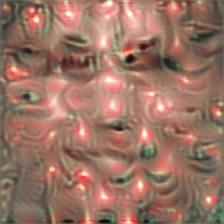
\includegraphics[width=0.35\linewidth]{figures/images/squ_fail}
\caption[Artefakti na slikah ob uporabi kritika]{Artefakti na slikah ob uporabi kritika}
\label{fig:squ_fail}
\end{figure}

Na generiranih slikah so se namreč pojavljali artefakti, ki so popolnoma pokvarili videz slike.
\\\ 
Razloga za pojav artefaktov nismo poznali, zato smo poskušali implementirati kritika s pomočjo druge klasifikacijske mreže. Poskušali smo z dvema mrežama, \textbf{VGG-FACE} deskriptor \cite{parkhi2015deep} in  \textbf{Inception-V3} \cite{szegedy2016rethinking}. VGG  arhitektura \cite{simonyan2014very} na vhod dobi trikanalno RGB sliko velikost 224x224 slikovnih točk. Sliko pošljemo skozi zaporedje več konvolucijsih slojev, kjer so uporabljeni filtri zelo majhne velikosti, praviloma 3x3.To je najmanjša velikost jedra, ki še omogoča zajemanje gibanja. Nekaterim konvolucijskim slojem  sledijo  t.i.  angl. max-pooling sloji, ki imajo okno velikosti 2x2 z nastavljenim preskokom 2.  Zaporedju teh konvolucijskih slojev sledijo trije polnopovezavni sloji. Prva dva sta velikost 4096, tretji pa velikost 1000, saj je zadolžen za klasifikacijo problema s toliko razredi. Zadnji sloj je t.i. softmax sloj. Vsi notranji sloji uporabljajo \textit{ReLU} aktivacijo. 
\\ Imamo več različic VGG arhitekture, katerih glavna razlika pa je le skupno število konvolucijskih slojev, ki se pojavljajo v mreži. V našem primeru smo uporabili VGG-16 arhitekturo. 
\\
Največja prednost Inception  arhitekture  v primerjavi  z VGG arhitekturo je drastično manjše število parametrov, vendar za ceno  veliko večja kompleksnost arhitekture. To nam oteži spreminjanje mreže, da bi bolje ustrezala novim namenom. 
Vse podrobnosti o arhitekturi so natančno opisane v \cite{szegedy2016rethinking}. 
\\ 
V našem primeru smo dobili prednaučeni mreži, ki so bile učeni na \cite{parkhi2015deep} učni mmnožica. Implementacija in prednaučeni modeli  tako VGG-Face kot Squeezenet arhitekture omenjene zgoraj je pridobljena iz \cite{grm2017strengths}.
\\
Žal se rezultati, ki smo jih dobili v skupnem modelu niso drastično izboljšali. Kljub velikim spremebam v arhitekturi kritika, se artefaktov nismo mogli znebiti. Opazili smo samo spremembo v sami obliki artefaktov, predvsem pri uporabi InceptionV3 arhitekture.

\begin{figure}
\centering
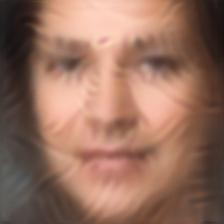
\includegraphics[width=0.35\linewidth]{figures/images/inception_artifacts.jpg}
\caption[Artefakti na slikah ob uporabi InceptionV3 mreže]{Artefakti na slikah ob uporabi InceptionV3 mreže}
\label{fig:squ_fail}
\end{figure}



% RABIM TUKI SUBSUBSECTION?? 
\subsubsection{Učenje kritika na isti bazi}
Problem je bil očitno neodvisen od arhitekture kritika, zato je bilo težavo potrebno reševati na drugačen način. 
Želeli smo kritika naučiti na isti množici, kot jo uporabljamo za učenje staranja.
Težava je nastala pri iskanju primerne podatkovne baze. Ta je namreč potrebovala tako anotacije za starost kot anotacije za identiteto. Potrebno je bilo, da imamo v bazi osebe, ki so predstavljene z večimi slikami. To je potrebno za učenje identitetnega klasifikatorja. Ideja je bila, da naučimo klasifikator ter podobno kot v prejšnjem primeru vzamemo značilke iz zadnjega polnopovezanega sloja, ter s kosinusno razdaljo primerjamo razdalje med osebami. 
\\
Odločili smo se za uporabo  \textbf{IMDB-WIKI} podatkovne baze \cite{Rothe-IJCV-2016}, ki vsebuje fotografije oseb, ki so pridobljene iz spletnih strani IMDB ter Wikipedia. Osnovna baza vsebuje slike oseb, kjer je lahko obraz le manjši del slik. Uporabljali pa smo različico baze, kjer so slike avtomatsko obrezane tako, da so na slikah samo obrazi.  
\\
Zaradi pomanjkanja človeškega nadzora, imamo v bazi tudi slike, kjer ni obraza. Vsaka slika je anotirana s parameterom \textit{face\_score}, ki je metrika, katera meri prisotnost obraza na sliki. Na ta parameter se zanašamo, da iz baze porežemo slike katere niso primerne. Želimo nastaviti spodnjo mejo za vrednost, tako da bomo dobili dobro razmerje med številom obdržanih slik ter kvaliteto le-teh. Mejo smo eksperimentalno nastavili na 3. 
\\
Preden smo zgradili celotni model s kritikom, smo preizkusili novo podatkovno bazo kot učno množico za konvolucijski variacijski autoenkoder, ki je  bil predstavljen zgoraj. Kmalu smo ugotovili, da je kvaliteta generiranih slik precej slabša kot pri uporabi \textit{UTKFace} baze. Razlog je predvem v tem, da so tam slike že predhodno poravnane. Kazalo je, da je neporavnanost slik velik problem, saj nam je mreža generirala slike, ki so bile popolnoma neostre \ref{fig:non-aligned-imdb}

\begin{figure}
\centering
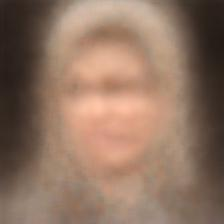
\includegraphics[width=0.30\linewidth]{figures/images/non_aligned_imdb.jpg}
\caption[Generirane slike, kadar učna množica ni vsebovala poravnanih slik]{Generirane slike, kadar učna množica ni vsebovala poravnanih slik}
\label{fig:non-aligned-imdb}
\end{figure}

Izgledalo je, da ima mreža težave pri učenju obraza, kadar so obrazi na učnih slikah različnih dimenzij, pozicij, osvetlitev in velikosti.
\\
Da bi  lahko podatkovno bazo uporabljali za naš generativni model, smo potrebovali implementirati poravnavo obrazov na slikah v učni množici. 
Uporabili smo angl. \textbf{Dlib face landmarks}, ki nam poda lastnosti ključnih elementov na obrazih oseb. To lahko uporabljamo za iskanje teh elementov na podani sliki. V našem primeru potrebujemo zaznati položaj notranjih kotičkov oči ter koncev spodnje ustnice. Slike bodo poravnane, kadar bodo zaznani elementi na istem mestu na vseh slikah v množici. To storimo z linearnimi transformacijami, ki točke projecirajo na isto mesto.  Do težav sicer pride pri slikah, kjer so osebe fotografirane iz strani, saj projekcija precej pokvari kvaliteto slike, vendar je to potreben kompromis za uporabo naše podatkovne baze. 
\\
Ko smo imeli poravnane obrazne slike, smo morali uporabiti poravnane slike za učenje klasifikatorja, ki se bo uporabljal kot naš kritik. V bazi smo najprej morali določiti osebe, za katere smo imeli na voljo zadostno število različnih fotografij, saj le-tako lahko pravilno naučimo identitetni klasifikator. Tudi tukaj smo morali določiti koliko slik iste osebe potrebujemo da pravilno naučimo identifikacijo obrazov. Izbrali smo mejo vsaj 75  slik na osebo, kar naj bi glede na prejšnje izkušnje zadostovalo za učenje klasifikatorja ter ohranilo zadostno število fotografij v bazi, da je učenje variacijskega autoenkdoerja še vedno mogoče. 
\\
Najprej smo se odločili za učenje Squeezenet arhitekture, ki je bila opisana zgoraj, vendar  nam ni uspelo doseči konvergence. Poizkušali smo z različnimi parametri za število slik na osebo, poizkušali smo z dodatno normalizacijo, vendar se natančnost klasifikacije ni povzpela prek 10\%. Podobno je veljalo pri  VGG-16 arhitekturi, kjer so se pojavlile popolnoma iste težave pri učenju klasifikatorja. 
Predvidevamo, da je največji razlog slaba kvaliteta slik v učni množici, kar neomogoča klasifikatorju, da bi dosegel konvergenco. 
\\
Več uspeha smo imeli z učenjem \textbf{Inception-V3}  klasifikatorja. Tukaj je konvergenca lepo napredovala in dobili smo približno 90 odstotno klasifikacijsko natančnost. Za naše namene bi moralo to zadostovati, saj je naloga klasifikatorja, da se vede kot kritik in samo usmerja učenje v pravo smer.  
\\
Naš model smo torej sestavili iz konvolucijskega variacijskega autoenkoderja povezanega s kritikom, zgrajenim s pomočjo \textbf{Inception-V3} arhitekture. Poizkušali smo pravilno utežiti razmerje med kriterijem kritika, rekonstrukcijo napako ter KL divergenco, vendar nam ni uspelo pridobiti rezultatov ki bi izboljšali naše generirane slike. Ob manjši utežitvi kritika,  so generirane slike bile popolnoma iste kot pri modelu kjer kritik ni dodan. Ob večji utežitvi pa so se znova začeli pojavljati artefakti. Sicer ti  niso bili tako močno opazni, kot pri prejšnjih pristopih, vendar je bila njihova prisotnost vseeno vidna. 
\\
Zaradi spremembe baze, se je  precej poslabšala tudi kvaliteta generiranih obrazov, zaradi slabše podatkovne baze. Prav tako, je problem predstavljalo generiranje najbolj mladih oz. starih obrazov. Problem je zaradi neuravnoteženosti baze, kar se tiče starostnih porazdelitev. Ker so slike pobrane iz strani IMDB in Wikipedia imamo v bazi zelo malo slik otrok, saj je relativno gledano precej manj otrok, ki nastopajo kot igralci oz. so dovolj znani/pomembni, da bi imeli svojo stan na spletni enciklopediji Wikipedia.  
\\
Zaradi omenjienih težav in neuspešnega poskusa z uvedbo kritika, ki ga naučimo sami, smo se odločili da se vrnemo na uporabo UTKFace podatkovne baze in poskušamo s preizkušanjem alternativnih pristopov. 

\subsection{Variacijski autoenkoder s konsistentimi globokimi značilkami}

Implementirali in preizkusili smo delovanje še ene razširitve klasičnega variacijskega autoenkoderja in sicer variacijski autoenkoder s konsistentinimi globokimi značilkami, angl. deep feature consistent (DFC), variacijski autoenkoder \cite{hou2017deep}. V članku avtorji predstavijo idejo, kjer spremenijo klasično kriterijsko funkcijo variacijskega autoenkoderja tako, da navadno rekonstrukcijsko napaka zamenjajo s kriterijem  ujemanja globokih značilk. 
Koliko sta si dve sliki podobni lahko definiramo skozi ujemanje značilk, ki  se pojavljajo v notranjih slojih nevronskih mrež. Želimo poiskati podobnosti med globokimi reprezentacijami slike.  Naj  $\Phi(x)^l$ predstavljajo vrednosti v $l$-tem skritem  sloju nevronske mreže $\Phi$ pri vhodu $x$. Matematično gledano je $\Phi(x)^l$ 3-dimenzionalni kvader oblike $[C^l \times
W^l \times H^l]$, kjer $C^l$  predstavlja število filtrov, $W^l$ in $H^l$ pa širino in višino značilk na $l$-tem nivoju konvolucijske mreže.  
Kriterijsko funkcijo za en sloj ($\mathcal{L}_{\text{rec}}^l $) lahko definiramo kot evklidsko razdaljo med dvema slojema.
Velja torej
\begin{equation}
\mathcal{L}_{\text{rec}}^l (x,\hat{x}) = \frac{1}{2C^lW^lH^l} \sum_{c=1}^{C^l}\sum_{w=1}^{W^l}\sum_{h=1}^{H^l}(\Phi(x)^l_{c,w,h} 
- \Phi(\hat{x}^l_{c,w,h})^2
\label{eq:dfc-layer}
\end{equation}

Končna rekonstrukcijska napaka je definirana kot vsota takih enoslojnih rekonstrukcijskih napak  $L_{\text{rec}} = \sum_l \mathcal{L}_{\text{rec}}^l$. 
Za učenje variacijskega autoenkdoerja moramo skupaj minimizirati KL divergenco ter rekonstrukcijsko napako, kot smo jo definirali. Skupna kriterijska funkcija je torej 
\begin{equation}
\mathcal{L} = \alpha\mathcal{L}_{kl} + \beta \sum_i^l{\mathcal{L}_{rec}^l}
\end{equation}

kjer sta $\alpha$ in $\beta$ uteži, ki določata kateremu delu bomo dali več pomembnosti. 
\\ 
Zanimalo nas je, če bi novo definirani $\mathcal{L}_{rec}$  lahko uporabili kot dodatno kriterijska funkcija za ohranjanje identitete. Pustili bi klasično rekonstrukcijsko napako ter dodali novo napako, ki naj bi bila zadolžena za primerjanje identitete med dvema obrazoma. S tem bi poizkušali še bolj posplošiti pristop s kritikom. Definirali smo novo kriterijsko funkcijo, ki jo zapišemo 
\begin{equation}
\mathcal{L} = \alpha \mathcal{L}_{kl} + \beta \mathcal{L}_{rec} + \gamma\sum_i^l(\mathcal{L}_{rec}^l) 
\end{equation}

Kot so to storili avtorji v članku, smo želeli metodo preizkusiti na \textit{VGG-16} in \textit{VGG-19} arhitekturah. 
Implementirali smo več različnih verzij DFC kritika. Pomembno je število oz. izbira notranjih slojev, ki jih primerjamo med sabo. Naredili smo tri različice 
\begin{itemize}
\item \textbf{VAE-123}, kjer smo med sabo primerjali prvi tri konvolucijske sloje v VGG mreži
\item\textbf{VAE-456}, kjer smo med sabo primerjali zadnje tri konvolucijske bloke v VGG mreži
\item \textbf{VAE-all}, kjer smo primerjali vse konvolucijske bloke med sabo. 
\end{itemize}

Pomembno je na kakšnih podatkih, je naučena \textit{VGG} mreža. Najprej smo metodo preizkusili na prednaučeni mreži, ki smo jo uporabljali že v prejšnjem pristopu \cite{grm2017strengths}. Implementacijo mreže je bilo potrebno nadgraditi tako, da smo namesto končnega sloja, vračali podatke iz potrebnih notranjih slojev. 
\\
Vsako od slik učne množice smo dali na vhod tej mreži, ter dobili seznam vektorjev potrebnih notranjih slojev. Poleg vhodne slike ter starosti, smo to uporabljali kot dodatni vhod našega celotnega modela, da smo lahko te podatke uporabljali v naši kriterijski funkciji. Kot vidimo v enačbi \ref{eq:dfc-layer}, je potrebno vsakega od upoštevanih slojev primerno normalizirati glede na njegovo velikost. Zaradi notranjih omejitev knjižnice \textit{Keras}, v kriterijski funkciji ni bilo mogoče dostopati do dimenzije trenutnega tenzorja. Uteževanje smo naredili ročno, tako da smo predhodno dobili dimenzije notranjih slojev, si to vrednost zapomnili, ter končni sloj utežili s primerno fiksno prednastavljeno vrednostjo. 
Pristop je ekvivalenten, vendar zahteva ročno spreminjanje uteži, če  spremenimo vhodne dimenzije našega modela. 
\\ 
V \cite{hou2017deep} je omenjeno, da med učenjem uporabljamo  KL divergenco za učenje enkoderja, ter rekonstrukcijsko napako za učenje tako enkoderja kot dekoderja. 
\\
Implementacijsko gledano, moramo v knjižnici Keras ustvariti dva modela. Prvi je zadolžen za učenje s pomočjo KL divergence,  ter vsebuje samo sloje enkoderja, drugi pa posodablja celotno mrežo s pomočjo rekonstrukcijske napake. 
\\
V našem primeru smo kot rekonstrukcijsko napako definirali uteženo razmerje med klasično rekonstrukcijsko napako osnovano na primerjavi posameznih slikovnih točk ter med novo uvedeno primerjavo globokih značilk. 
\\
Mrežo smo učili s pomočjo optimizatorja \textbf{ADAM} z učno hitrostjo  0.0005. Ostali parametri so ostali isti kot pri implementaciji klasičnega variacijskega autoenkoderja. 
Zaradi nezadovoljivih rezultatov dobljenih s pomočjo tega pristopa, kjer so slike delovale precej  smo najprej želeli spremeniti prednaučenega kritika. V članku je omenjeno, da so avtorji uporabljali  mrežo, ki se bila prednaučena s pomočjo \textbf{ImageNet} \cite{russakovsky2015imagenet} podatkovne množice. 
\\
Orodje Keras ima notranjo implementacijo \textbf{VGG-16} ter \textbf{VGG-19} arhitektur, ki uporabljajo prednaučene ImageNet uteži. Ker ta ne omogoča dostopa do notranjih slojev, smo njihovo implementacijo nadgradili z dodatnim parametrom, ki je omogočal dostop do notranjih slojev nevronske mreže. 
Rezultati niso bili takšni, kot bi si jih želeli, saj so obrazi  izgledale kot narisanim kot je vidno na sliki \ref{fig:dfc-cartoon}. Zato smo se odločili preizkusiti še implementacijo, ki je bila definirana v članku, kjer imamo samo eno rekonstrukcijsko napako, osnovano na primerjavi notranjih slojev. Ostale implementacijske podrobnosti pa so ostale enake.  


\begin{figure}
\centering
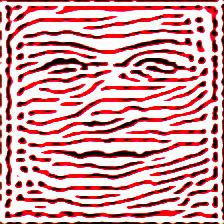
\includegraphics[width=0.30\linewidth]{figures/images/dfc_wtf.jpg}
\caption[Risankasta podoba obrazov, pri uporabi DFC autoenkoderja]{Risankasta podoba obrazov, pri uporabi DFC autoenkoderja}
\label{fig:dfc-cartoon}
\end{figure}


\section{Autoenkoder}
Zaradi nezadovoljivih rezultatov, dobljenih s pomočjo različic variacijskih autoenkoderjev smo začeli raziskovati možne inačice autoenkoderjev.  Najprej smo naredili povsem klasičen pogojni konvolucijski autoenkoder, kot je viden na sliki --VSTAVI SLIKO -- 
Uporabljali smo \textit{adadelta} optimizator ter binarno krosentropijo za kriterijsko funkcijo. Našo mrežo smo učili s svežnji velikosti 32 ter postopek učili 30 epoch-ov.  Velikost vhodnih in izhodnih podatkov je v tem primeru povsem nastavljiva, vendar smo kot osnovo izbrali velikost silk 224 x 224 slikovnih točk. Pomembna je tudi velikost latentnega vektorja, ki smo jo nastavili na 64, kjer je zadnjih 10 elementov vektorja zadolženih za shranjevanje informacije, ki določa starostni razred. 
\\ 
Implementirali smo tudi razširjeno verzijo autoenkoderja, ki je bila osnova na DFC implementaciji, kjer smo poleg binarne krosentropije uporabljali tudi rekonstrukcijsko napako, ko je definirana v poglavju o variacijskih autoenkoderjih s konsistentnimi globokimi značilkami.  Parametri ter arhitektura je ostala enaka, edina sprememba je v strukturi modela ter v razširitvi kriterijske funkcije. 

\subsection{Nasprotniški autoenkoder}
Naredili smo nasprotniški autoenkoder, ki je osnovan na konvolucijski arhitekturi.  Na vhod smo podajali barvne slike velikosti 224 x 224 slikovnih točk  ter oznake o starosti oseb.   V primeru nasprotniškega autoenkoderja je mreža sestavljena iz treh glavnih delov
\begin{itemize}
\item Enkoder $E$, ki je zadolžen, da se vhodni podatki zakodirajo v latentno reprezentacijo
\item Generator (dekoder) $G$, ki je zadolžen za generiranje slike iz latentne reprezentacije
\item Diskriminator $D$, ki je zadolžen za ohranjanje enotske naravne porazdelitve latentnega vektorja 
\end{itemize}

Vsak od teh delov ima svojo arhitekturo. Če pogledamo sliko -- referenca na enkoder -- vidimo, da je sestavljen iz treh zaporednih konvolucijskih slojev, nato pa reprezentacijo sploščimo in iz nje naredimo dva polnopovezana sloja srednje vrednosti ter variance. Uporabljamo torej normalno porazdeljeni enkoder, kot je definiran v enačbi \ref{eq:aae-normal}.


%---------------------------------------------------------------
% SLO: bibliografija
% ENG: bibliography
%----------------------------------------------------------------

%----------------------------------------------------------------
% SLO: odkomentiraj za uporabo zunanje datoteke .bib (ne pozabi je potem prevesti!)
% ENG: uncomment to use .bib file (don't forget to compile it!)
%----------------------------------------------------------------
\bibliography{bibliography}

%----------------------------------------------------------------
% SLO: zakomentiraj spodnji del, če uporabljaš zunanjo .bib datoteko
% ENG: comment the part below if using the .bib file
%----------------------------------------------------------------

\end{document}
